% =====================================================================
%  Joystick Signal Processing and Trajectory Pipeline
%  Center-out length categorization task (Merchant Lab)
%  Task suite centerTask v8.26 + EDA notebooks
% =====================================================================
\documentclass[11pt,a4paper]{article}

\usepackage[T1]{fontenc}
\usepackage[utf8]{inputenc}
\IfFileExists{lmodern.sty}{\usepackage{lmodern}\usepackage{microtype}}{\usepackage[expansion=false]{microtype}}
\usepackage[margin=2.4cm]{geometry}

\usepackage{amsmath,amssymb,bm}
\usepackage{booktabs}
\usepackage{longtable}
\usepackage{array}
\usepackage{multirow}
\usepackage{enumitem}
\usepackage{xcolor}
\usepackage{graphicx}
\usepackage{caption}
\usepackage{listings}
\usepackage[ruled,vlined,linesnumbered]{algorithm2e}
\usepackage{tikz}
\usepackage{pgfplots}
\pgfplotsset{compat=1.18}
\usetikzlibrary{arrows.meta,positioning,calc,fit,backgrounds,shapes.geometric,
                decorations.pathreplacing,decorations.markings,patterns}
\usepackage{float}
\usepackage[colorlinks=true]{hyperref}

% ---------------------------------------------------------------- colours
% Pastel palette (as in the previous edition of this document): every fill is
% a light pastel and every stroke is that same pastel darkened, never a tint,
% so borders stay visible against the fill.
\definecolor{pblue}{HTML}{BFD7EA}   \definecolor{pblued}{HTML}{5B8DB8}
\definecolor{pgreen}{HTML}{C7E9C0}  \definecolor{pgreend}{HTML}{5FA36B}
\definecolor{ppink}{HTML}{F9C6D0}   \definecolor{ppinkd}{HTML}{C96A82}
\definecolor{pyellow}{HTML}{FBE7A1} \definecolor{pyellowd}{HTML}{C9A227}
\definecolor{ppurple}{HTML}{D9C8EA} \definecolor{ppurpled}{HTML}{8A6BB1}
\definecolor{porange}{HTML}{FBD5B5} \definecolor{poranged}{HTML}{D68B4A}
\definecolor{pgray}{HTML}{E6E6E6}   \definecolor{pgrayd}{HTML}{7A7A7A}
\definecolor{pteal}{HTML}{BFE3DE}   \definecolor{ptealed}{HTML}{4E948C}

% Short aliases used throughout the figures.
\colorlet{dblue}{pblued}   \colorlet{dgreen}{pgreend}
\colorlet{dpink}{ppinkd}   \colorlet{dyellow}{pyellowd}
\colorlet{dpurple}{ppurpled}\colorlet{dorange}{poranged}
\colorlet{dgray}{pgrayd}   \colorlet{dteal}{ptealed}

\definecolor{codebg}{HTML}{F1F1F1}
\definecolor{codekw}{HTML}{5B8DB8}
\definecolor{codecom}{HTML}{7A7A7A}
\definecolor{codestr}{HTML}{C96A82}

\hypersetup{linkcolor=pblued,citecolor=pgreend,urlcolor=ppurpled}

% ---------------------------------------------------------------- listings
\lstdefinestyle{src}{
  backgroundcolor=\color{pgray!40},
  basicstyle=\ttfamily\footnotesize,
  keywordstyle=\color{codekw}\bfseries,
  commentstyle=\color{codecom}\itshape,
  stringstyle=\color{codestr},
  frame=single,
  rulecolor=\color{pgrayd},
  framerule=0.3pt,
  framesep=4pt,
  breaklines=true,
  columns=fullflexible,
  keepspaces=true,
  showstringspaces=false,
  xleftmargin=4pt,
  xrightmargin=4pt,
  aboveskip=9pt,
  belowskip=9pt,
}
\lstset{style=src}

% ---------------------------------------------------------------- tikz styles
\tikzset{
  % Filled pastel node with a darkened stroke of the same hue.
  blk/.style   = {rectangle, rounded corners=3pt, draw=#1!70!black, fill=#1, thick,
                  align=center, inner sep=5pt, font=\footnotesize, minimum height=9mm},
  blk/.default = pgray,
  box/.style   = {rectangle, rounded corners=3pt, draw=#1!70!black, fill=#1, thick,
                  align=center, inner sep=5pt, font=\small, minimum height=9mm},
  box/.default = pgray,
  file/.style  = {draw=pgrayd, fill=pgray, thick, inner sep=5pt, align=center,
                  font=\footnotesize\ttfamily},
  lane/.style  = {-{Latex[length=2.5mm]}, thick, pgrayd},
  arr/.style   = {-{Latex[length=2.5mm]}, thick, pgrayd},
  thin lane/.style = {-{Latex[length=2mm]}, pgrayd},
  note/.style  = {font=\scriptsize\itshape, text=pgrayd, align=center},
  tag/.style   = {font=\scriptsize, text=pgrayd, align=center},
  lbl/.style   = {font=\scriptsize, text=pgrayd, align=center},
  pt/.style    = {circle, fill=pblued, inner sep=1.4pt},
  spike/.style = {circle, fill=ppinkd, inner sep=1.8pt},
}

% Ragged-right paragraph columns: justified narrow columns produce the loose
% inter-word spacing that makes long tables look broken.
\newcolumntype{P}[1]{>{\raggedright\arraybackslash}p{#1}}

\captionsetup{font=small,labelfont=bf,width=0.94\textwidth}
\setlength{\parskip}{2pt}

% Long typewriter identifiers must be allowed to end a line without
% overflowing the margin; emergencystretch plus a raised tolerance is what
% keeps the paragraphs inside the text block.
\setlength{\emergencystretch}{3.2em}
\tolerance=1800
\hbadness=6000

\newcommand{\code}[1]{\texttt{\small #1}}
\newcommand{\file}[1]{\texttt{\small #1}}

\title{\bfseries Joystick Signal Processing and Trajectory Pipeline}
\author{Center-out length categorization task (Merchant Lab)\\
Task suite \code{centerTask v8.26} and the EDA notebooks}
\date{}

\begin{document}
\maketitle

\noindent
This document describes the joystick signal path as it works in the version
currently deployed: from the RZ2 analog-to-digital converter to the kinematic
quantities computed in the exploratory data analysis (EDA) notebooks. Every
transformation is stated first as a mathematical object, then located in the
code (file, class or function, and the variable that carries it), and finally
annotated with the parameters that control it.

\medskip
\noindent
The chain has two halves that live on different machines and in different
languages. The \emph{online} half (MATLAB, \file{centerTask/}) acquires the
signal and writes raw trajectories with hardware-derived timestamps; it applies
no filtering of any kind. The \emph{offline} half (Python, EDA notebooks,
section 1.1) cleans those trajectories and differentiates them. Because the
online side never alters the shape of the signal, the two halves can be reasoned
about independently, and the raw rows always remain in the exported file.

\tableofcontents
\newpage

% =====================================================================
\section{Notation and conventions}
% =====================================================================

\begin{center}
\small
\begin{tabular}{@{}llP{9.4cm}@{}}
\toprule
Symbol & Units & Meaning \\
\midrule
$f_s$ & Hz & RZ2 write rate of the joystick buffer. Seed value
  $24414.0625/26 = 939.0024$ Hz, re-estimated online by \code{RZ2ClockMap} \\
$a, b$ & s/sample, s & Slope and intercept of the affine clock map
  $\hat t(n) = b + a\,n$ (\file{RZ2ClockMap.m}) \\
$\varsigma_k$ & s & Clock skew measured at frame $k$:
  \code{sampleTime} $-$ \code{trigTime} (\file{ClockSkewMonitor.m}) \\
$n_i \in \mathbb{N}$ & samples & Monotone absolute sample index attached by the
  relay to sample $i$ \\
$(v_{x,i}, v_{y,i}) \in [-1,1]^2$ & (dimensionless) & Normalized joystick
  deflection of sample $i$ (normalization performed on Computer 1) \\
$t_i$ & s & Local (Computer 2) \code{GetSecs} time assigned to sample $i$ \\
$(x_i, y_i)$ & px & Screen coordinates of sample $i$ (origin top-left,
  $y$ grows downward) \\
$(x_c, y_c)$ & px & Screen centre \\
$W, H$ & px & Screen width and height ($1920$, $1080$) \\
$s_x, s_y, o_y$ & --, --, px & RZ2 gain on each axis and vertical offset
  (\code{rz2ScaleX}, \code{rz2ScaleY}, \code{rz2OffsetY}) \\
$T_0$ & s & \code{sessionT0}, the instant the first trial started \\
$\tau_i$ & ms & \code{Time\_ms} $= \max\!\big(1000\,(t_i - T_0),\, 0\big)$ \\
$\Delta t_k$ & s & Irregular step $t_k - t_{k-1}$ in the offline chain \\
$\Delta$ & s & Uniform resampling step ($0.008$ s, i.e.\ $125$ Hz) \\
$c$ & cm/px & Pixel pitch, $c = 0.3108\,\text{mm/px}/10 = 0.03108$ cm/px \\
\bottomrule
\end{tabular}
\end{center}

\noindent
Each axis is processed independently unless stated otherwise. Vectors are column
vectors and $\bm{I}$ is the identity.

% ---------------------------------------------------------------------
\subsection{The whole pipeline on one page}
% ---------------------------------------------------------------------

Figure~\ref{fig:onepage} is the map for everything that follows. Two quantities
travel from left to right and each boundary transforms exactly one of them: the
\emph{value} of the joystick signal changes units (volts, then $[-1,1]$, then
pixels, then centimetres), and its \emph{time} changes reference (ADC sample
index, then Computer~2's clock, then milliseconds since the first trial, then a
uniform 125~Hz grid). Nothing on the online side changes the \emph{shape} of the
signal; every filter is offline, and it is reversible in the sense that the raw
rows remain in the file.

\begin{figure}[htbp]
\centering
\resizebox{\textwidth}{!}{%
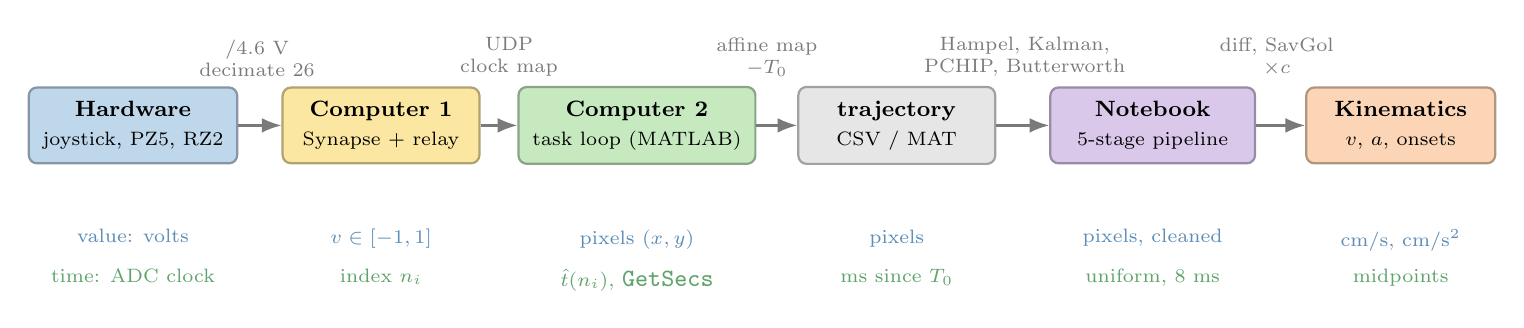
\begin{tikzpicture}[node distance=0pt]
% --- boxes, fixed x positions so nothing can overlap ------------------
\node[blk=pblue,   minimum width=25mm] (hw)   at (0.00,0) {\textbf{Hardware}\\[1pt]\scriptsize joystick, PZ5, RZ2};
\node[blk=pyellow, minimum width=25mm] (c1)   at (3.15,0) {\textbf{Computer 1}\\[1pt]\scriptsize Synapse + relay};
\node[blk=pgreen,  minimum width=27mm] (c2)   at (6.40,0) {\textbf{Computer 2}\\[1pt]\scriptsize task loop (MATLAB)};
\node[blk=pgray,   minimum width=25mm] (file) at (9.70,0) {\textbf{trajectory}\\[1pt]\scriptsize CSV / MAT};
\node[blk=ppurple, minimum width=26mm] (nb)   at (12.95,0){\textbf{Notebook}\\[1pt]\scriptsize 5-stage pipeline};
\node[blk=porange, minimum width=24mm] (kin)  at (16.10,0){\textbf{Kinematics}\\[1pt]\scriptsize $v$, $a$, onsets};

% --- arrows -----------------------------------------------------------
\foreach \a/\b in {hw/c1, c1/c2, c2/file, file/nb, nb/kin} {\draw[lane] (\a) -- (\b);}

% --- labels above the arrows -----------------------------------------
\node[tag, above=5mm of $(hw)!0.5!(c1)$]   {$/4.6$ V\\decimate 26};
\node[tag, above=5mm of $(c1)!0.5!(c2)$]   {UDP\\clock map};
\node[tag, above=5mm of $(c2)!0.5!(file)$] {affine map\\$-T_0$};
\node[tag, above=5mm of $(file)!0.5!(nb)$] {Hampel, Kalman,\\PCHIP, Butterworth};
\node[tag, above=5mm of $(nb)!0.5!(kin)$]  {diff, SavGol\\$\times c$};

% --- value lane -------------------------------------------------------
\node[tag, text=dblue, below=7mm of hw]   (v1) {value: volts};
\node[tag, text=dblue, below=7mm of c1]   (v2) {$v \in [-1,1]$};
\node[tag, text=dblue, below=7mm of c2]   (v3) {pixels $(x,y)$};
\node[tag, text=dblue, below=7mm of file] (v4) {pixels};
\node[tag, text=dblue, below=7mm of nb]   (v5) {pixels, cleaned};
\node[tag, text=dblue, below=7mm of kin]  (v6) {cm/s, cm/s$^2$};

% --- time lane --------------------------------------------------------
\node[tag, text=dgreen, below=12mm of hw]   {time: ADC clock};
\node[tag, text=dgreen, below=12mm of c1]   {index $n_i$};
\node[tag, text=dgreen, below=12mm of c2]   {$\hat t(n_i)$, \code{GetSecs}};
\node[tag, text=dgreen, below=12mm of file] {ms since $T_0$};
\node[tag, text=dgreen, below=12mm of nb]   {uniform, 8 ms};
\node[tag, text=dgreen, below=12mm of kin]  {midpoints};
\end{tikzpicture}}
\caption{The signal's two coordinates, value (blue lane) and time (green lane),
and what each boundary does to them. Sections~\ref{sec:online}--\ref{sec:read}
cover the first three boxes, \S\ref{sec:buffer} the file, and
\S\ref{sec:offline}--\S\ref{sec:downstream} the last two.}
\label{fig:onepage}
\end{figure}

% =====================================================================
\section{Online chain: from the ADC to the trajectory file}
\label{sec:online}
% =====================================================================

% ---------------------------------------------------------------------
\subsection{System overview}
% ---------------------------------------------------------------------

Figure~\ref{fig:chain} shows the two-machine link. Computer~1 (Windows) hosts
TDT Synapse; the gizmos \code{APICh1X} and \code{APICh2Y} write the joystick's
two analog channels into a ring buffer (\code{SerStore}) at $f_s$. A MATLAB
relay (\file{StepJoystickRelay.m}, \S\ref{sec:c1}) reads new samples from that
ring buffer through the write-index tag and pushes them over UDP to Computer~2
(Linux, Psychtoolbox), which only listens. The task loop on Computer~2 drains
the socket once per rendered frame, renders the newest sample, and logs
\emph{every} sample to the trajectory buffer.

\begin{figure}[htbp]
\centering
\resizebox{\textwidth}{!}{%
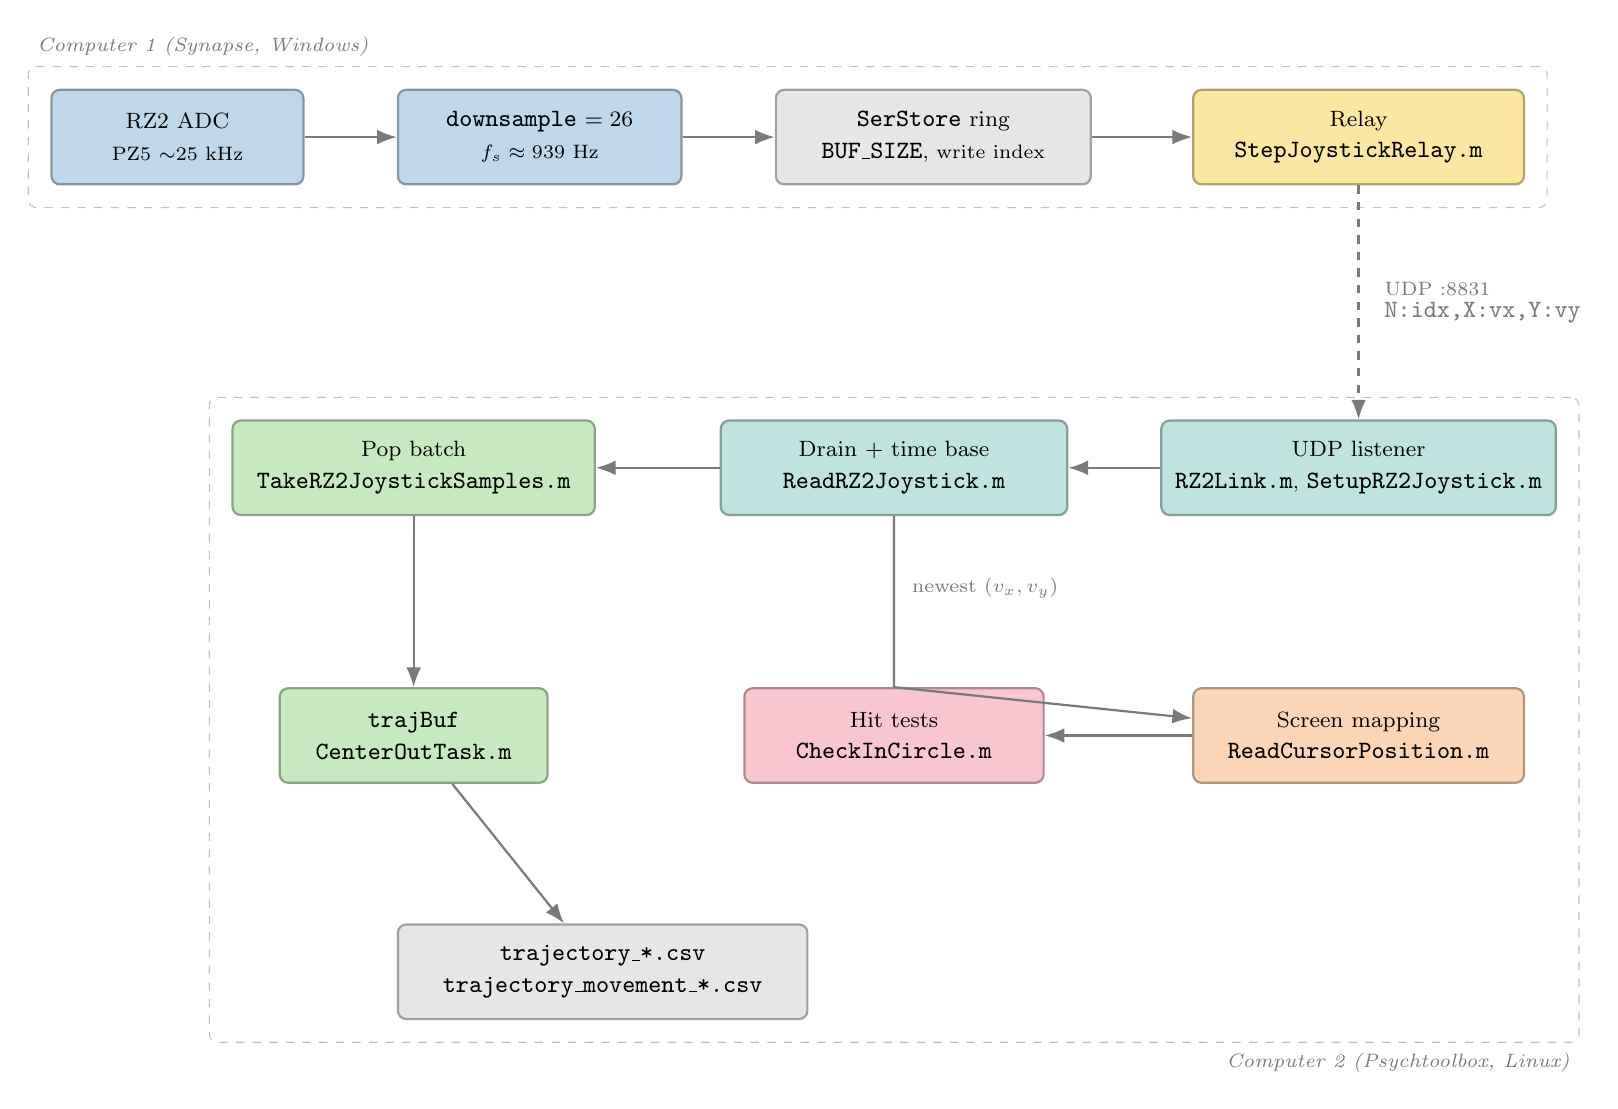
\begin{tikzpicture}[blk/.append style={minimum height=12mm}]
% ---- Computer 1 row (y = 0) -----------------------------------------
\node[blk=pblue,   minimum width=32mm] (adc)  at (0.0, 0) {RZ2 ADC\\[2pt]\scriptsize PZ5 $\sim$25 kHz};
\node[blk=pblue,   minimum width=36mm] (dec)  at (4.6, 0) {\code{downsample} $= 26$\\[2pt]\scriptsize $f_s \approx 939$ Hz};
\node[blk=pgray,   minimum width=40mm] (ring) at (9.6, 0) {\code{SerStore} ring\\[2pt]\scriptsize \code{BUF\_SIZE}, write index};
\node[blk=pyellow, minimum width=42mm] (relay)at (15.0,0) {Relay\\[2pt]\scriptsize \file{StepJoystickRelay.m}};
\foreach \a/\b in {adc/dec, dec/ring, ring/relay} {\draw[lane] (\a) -- (\b);}
\begin{scope}[on background layer]
  \node[draw=dblue!50, dashed, rounded corners=3pt, inner sep=8pt,
        fit=(adc)(dec)(ring)(relay)] (box1) {};
\end{scope}
\node[note, anchor=south west] at (box1.north west) {Computer 1 (Synapse, Windows)};

% ---- Computer 2, first row (y = -4.2) -------------------------------
\node[blk=pteal,   minimum width=42mm] (lis)  at (15.0,-4.2) {UDP listener\\[2pt]\scriptsize \file{RZ2Link.m}, \file{SetupRZ2Joystick.m}};
\node[blk=pteal,   minimum width=44mm] (drain)at (9.1, -4.2) {Drain $+$ time base\\[2pt]\scriptsize \file{ReadRZ2Joystick.m}};
\node[blk=pgreen,  minimum width=46mm] (pop)  at (3.0, -4.2) {Pop batch\\[2pt]\scriptsize \file{TakeRZ2JoystickSamples.m}};
\foreach \a/\b in {lis/drain, drain/pop} {\draw[lane] (\a) -- (\b);}

% ---- Computer 2, second row (y = -7.6) ------------------------------
\node[blk=pgreen,  minimum width=34mm] (traj) at (3.0, -7.6) {\code{trajBuf}\\[2pt]\scriptsize \file{CenterOutTask.m}};
\node[blk=ppink,   minimum width=38mm] (hit)  at (9.1, -7.6) {Hit tests\\[2pt]\scriptsize \file{CheckInCircle.m}};
\node[blk=porange, minimum width=42mm] (map)  at (15.0,-7.6) {Screen mapping\\[2pt]\scriptsize \file{ReadCursorPosition.m}};
\draw[lane] (pop) -- (traj);
\draw[lane] (map) -- (hit);
\draw[lane] (drain.south) -- node[tag, right=1mm, pos=0.42] {newest $(v_x,v_y)$} (map.north -| drain.south) -- (map);

% ---- Computer 2, third row (y = -10.6) ------------------------------
\node[blk=pgray,   minimum width=52mm] (csv)  at (5.4, -10.6)
     {\file{trajectory\_*.csv}\\[2pt]\scriptsize \file{trajectory\_movement\_*.csv}};
\draw[lane] (traj) -- (csv);

\begin{scope}[on background layer]
  \node[draw=dteal!50, dashed, rounded corners=3pt, inner sep=8pt,
        fit=(lis)(drain)(pop)(traj)(map)(hit)(csv)] (box2) {};
\end{scope}
\node[note, anchor=north east] at (box2.south east) {Computer 2 (Psychtoolbox, Linux)};

% ---- link between the two boxes -------------------------------------
\draw[lane, dashed] (relay) -- node[tag, right=2mm, align=left]
      {UDP :8831\\\code{N:idx,X:vx,Y:vy}} (lis);
\end{tikzpicture}}
\caption{Acquisition and logging chain. Nothing in this chain filters the
signal; it only timestamps, scales and stores. The drain feeds two consumers:
the newest sample goes to the screen map and the hit tests, and the whole batch
goes to the trajectory buffer.}
\label{fig:chain}
\end{figure}

% ---------------------------------------------------------------------
\subsection{Wire format and normalization}
% ---------------------------------------------------------------------

Each UDP datagram carries one relay cycle of samples, one text line per sample:
\[
  \code{N:}n_i\code{,X:}v_{x,i}\code{,Y:}v_{y,i}\code{\textbackslash n}
  \qquad\text{with } v_{x,i}, v_{y,i} \in [-1,1].
\]
The normalization from ADC volts to $[-1,1]$ is performed on Computer~1
(\code{JOY\_RANGE} $= 4.6$ V in \file{InitJoystickRelay.m}; see
\S\ref{sec:c1}), so Computer~2 never sees a voltage. Parsing is a single
\code{sscanf} over the whole datagram followed by \code{reshapeRecords}, which
keeps only $\lfloor \text{numel}/3 \rfloor$ complete records: a datagram torn
mid-line yields fewer samples, never a fabricated one. Asking \code{sscanf} for
a fixed size would instead zero-pad the final incomplete record, turning
\code{"N:101,X:0.6"} into $[101;\,0.6;\,0]$, a plausible-looking sample that
puts the cursor at $Y=0$.

A relay that has not been updated sends one sample per datagram without an
index (\code{X:}$v_x$\code{,Y:}$v_y$). Those datagrams are still accepted, so
the two machines can be upgraded one at a time, and the samples are counted in
\code{UserData.nLegacyFmt}.

% ---------------------------------------------------------------------
\subsection{Time base: sample index to local time}
\label{sec:clock}
% ---------------------------------------------------------------------

The relay attaches a monotone index $n_i$ that counts ADC samples, so a
sample's capture time is an affine function of its index. This is the key
design decision of the online chain: a sample that sat in the receive queue for
200~ms still receives the time it was \emph{captured}, not the time it was
\emph{read}. Figure~\ref{fig:capture} contrasts the two.

\begin{figure}[htbp]
\centering
\resizebox{\textwidth}{!}{%
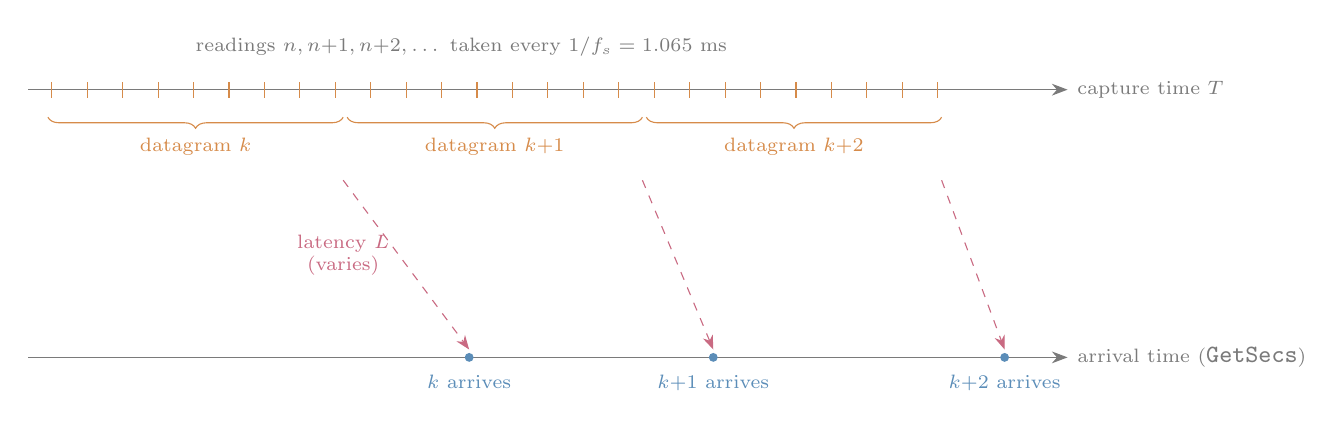
\begin{tikzpicture}[x=1cm,y=1cm]
% capture axis
\draw[-{Stealth[length=2mm]}, dgray] (0,0) -- (13.2,0) node[right, tag] {capture time $T$};
\foreach \x in {0.3,0.75,...,11.7} {\draw[dorange] (\x,-0.1) -- (\x,0.1);}
\node[tag, above=3mm of {(5.5,0)}] {readings $n, n{+}1, n{+}2, \dots$ taken every $1/f_s = 1.065$ ms};
% brackets
\draw[decorate, decoration={brace, amplitude=4pt}, dorange]
      (4.0,-0.35) -- (0.25,-0.35) node[midway, below=4pt, tag, text=dorange] {datagram $k$};
\draw[decorate, decoration={brace, amplitude=4pt}, dorange]
      (7.8,-0.35) -- (4.05,-0.35) node[midway, below=4pt, tag, text=dorange] {datagram $k{+}1$};
\draw[decorate, decoration={brace, amplitude=4pt}, dorange]
      (11.6,-0.35) -- (7.85,-0.35) node[midway, below=4pt, tag, text=dorange] {datagram $k{+}2$};
% arrival axis
\draw[-{Stealth[length=2mm]}, dgray] (0,-3.4) -- (13.2,-3.4) node[right, tag] {arrival time (\code{GetSecs})};
\foreach \s/\d in {4.0/5.6, 7.8/8.7, 11.6/12.4} {
  \draw[dashed, dpink, -{Stealth[length=1.8mm]}] (\s,-1.15) -- (\d,-3.3);
  \fill[dblue] (\d,-3.4) circle (1.6pt);
}
\node[tag, text=dblue, below=1mm of {(5.6,-3.4)}] {$k$ arrives};
\node[tag, text=dblue, below=1mm of {(8.7,-3.4)}] {$k{+}1$ arrives};
\node[tag, text=dblue, below=1mm of {(12.4,-3.4)}] {$k{+}2$ arrives};
\node[tag, text=dpink, align=center] at (4.0,-2.1) {latency $L$\\(varies)};
\end{tikzpicture}}
\caption{Capture time versus arrival time. Readings are taken at a fixed
cadence (top); datagrams arrive later and irregularly (bottom). The serial
number lets a reading recover its capture time no matter when its datagram
arrived.}
\label{fig:capture}
\end{figure}

Two things can make the two clocks disagree. A constant \emph{offset} is
harmless for durations (both ends shift equally) and biases
stimulus-to-response intervals by a constant. A \emph{rate} error is not
harmless: the disagreement grows every second and never stops growing. The
mechanism below removes the rate error and bounds what is left of the offset.

\subsubsection{The affine clock map}

\file{RZ2ClockMap.m} implements
\begin{equation}
  \hat t(n) \;=\; b + a\,n, \qquad a \approx 1/f_s \ \text{(seconds per sample)},
  \label{eq:affine}
\end{equation}
with $(a,b)$ refitted on every drain. Each drain $d$ contributes one observation
pair $(n^{(d)}, t^{(d)})$: the index of the \emph{newest} sample in the drain and
the \code{GetSecs} reading taken when the drain started. The newest sample is
the least delayed one in the batch (everything older sat behind it in the
queue), so it is the observation closest to the link's latency floor.
Observations live in a ring of $L = \code{rz2ClockWindow} = 600$ entries; refits
begin once at least \code{minObs} $=30$ observations are held.

\paragraph{Slope: the seed first.} Ordinary least squares over the window,
\begin{equation}
  a_{\mathrm{OLS}} = \frac{\sum_d (n^{(d)} - \bar n)(t^{(d)} - \bar t)}
                          {\sum_d (n^{(d)} - \bar n)^2},
  \qquad
  a = \operatorname{clip}\!\big(a_{\mathrm{OLS}},\; a_0(1-\delta),\; a_0(1+\delta)\big),
  \quad a_0 = \tfrac{1}{f_s^{\text{seed}}},\ \delta = 0.01,
  \label{eq:slope}
\end{equation}
but only once the window \emph{spans} at least
$\code{rz2ClockMinSpanSec} = 30$~s of samples; until then $a = a_0$. OLS is
unbiased for the slope even though every $t^{(d)}$ is contaminated by transport
latency, provided the latency is stationary, but unbiased is not precise. For a
window of $W$ observations spanning $S$ seconds with residual scatter
$\sigma_r$,
\begin{equation}
  \operatorname{se}(a) \;\approx\; \frac{\sigma_r}{\sigma_n \sqrt{W}},
  \qquad
  \sigma_n = \frac{f_s S}{\sqrt{12}},
  \label{eq:se}
\end{equation}
so a short window produces a slope that is mostly noise, while the seed is
known to a few hundred parts per million from the rig itself. The window earns
the right to change the slope only once its span makes the estimate better than
the seed.

\paragraph{Queue-clear gate.} The dangerous case is a \emph{growing} backlog.
Write the arrival time of the newest sample as its capture time plus a latency,
$t_{\mathrm{arr}}(n) = t_{\mathrm{cap}}(n) + L(n)$. If $L$ trends with $n$, the
fitted slope is
\begin{equation}
  a_{\mathrm{OLS}} \;\approx\; \frac{1}{f_s} + \frac{dL}{dn},
  \label{eq:gate}
\end{equation}
so the map attributes to a slower ADC what is really samples arriving later and
later. Its output then tracks \emph{arrivals} instead of captures,
\code{trigTime} stays close to \code{sampleTime}, and the skew monitor of
\S\ref{sec:skew} sees nothing: the one failure it exists to catch becomes
invisible. The estimator therefore refuses any observation from a drain that
did not leave the receive queue empty. The call is
\code{addObservation(idx, t, queueClear)} with
\code{queueClear = (backlog == 0)}, and refusals are counted in
\code{nObservationsRejected}. If the queue never clears, the map stops updating,
the estimate holds where it was, and the skew grows until the monitor stops the
session. Refusing to estimate is the correct response to data that cannot
support the estimate.

\paragraph{Intercept: a low quantile over a short window.} The intercept is
anchored on the $\code{rz2ClockOffsetQuantile} = 0.10$ quantile of the
residuals of the most recent $\code{rz2ClockOffsetWindow} = 100$ observations,
rather than on the OLS intercept:
\begin{equation}
  r_d = t^{(d)} - \big(b_{\mathrm{OLS}} + a\,n^{(d)}\big),
  \qquad
  b = b_{\mathrm{OLS}} + Q_{0.10}\big(\{r_d\}_{\text{last }100}\big).
  \label{eq:offset}
\end{equation}
$b_{\mathrm{OLS}}$ absorbs the \emph{mean} transport latency; a low quantile
tracks the fast path, which is the minimum-delay idea of clock
synchronisation, without the fragility of a strict minimum (a single early
packet or one corrupt index would drag it). The window is deliberately separate
from the slope window and much shorter: the slope needs span, the offset needs
to forget. A running minimum over a growing sample can only fall, which
ratchets the offset backwards; a window that actually slides cannot ratchet.
What survives in $b$ is only the unobservable, constant floor latency of the
link, which cancels in every within-trial difference.
Figure~\ref{fig:twowindows} shows the two windows over the same stream.

\begin{figure}[htbp]
\centering
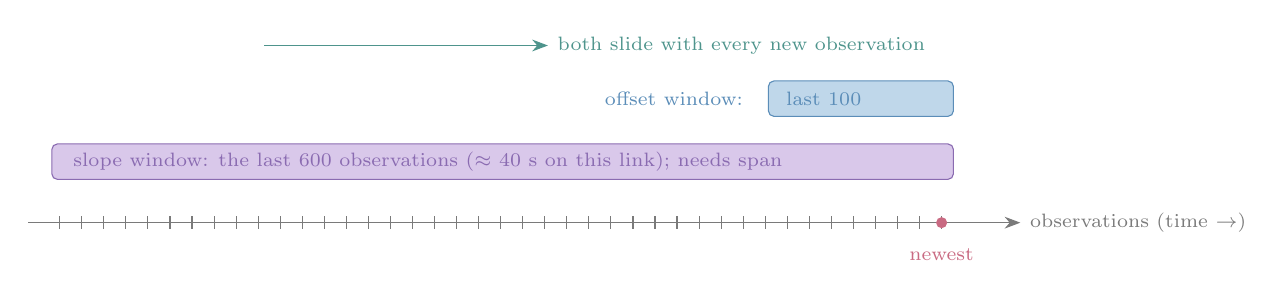
\begin{tikzpicture}[x=1cm,y=1cm]
\draw[-{Stealth[length=2mm]}, dgray] (0,0) -- (12.6,0) node[right, tag] {observations (time $\rightarrow$)};
\foreach \x in {0.4,0.68,...,11.6} {\draw[dgray] (\x,-0.08) -- (\x,0.08);}
\fill[dpink] (11.6,0) circle (2pt);
\node[tag, text=dpink, below=2mm of {(11.6,0)}] {newest};
% slope window
\draw[fill=ppurple, draw=dpurple, rounded corners=2pt] (0.3,0.55) rectangle (11.75,1.0);
\node[tag, text=dpurple, anchor=west] at (0.45,0.78)
      {slope window: the last 600 observations ($\approx$ 40 s on this link); needs span};
% offset window
\draw[fill=pblue, draw=dblue, rounded corners=2pt] (9.4,1.35) rectangle (11.75,1.8);
\node[tag, text=dblue, anchor=west] at (9.5,1.57) {last 100};
\node[tag, text=dblue, anchor=east] at (9.2,1.57) {offset window:};
% shared direction
\draw[-{Stealth[length=2mm]}, dteal] (3.0,2.25) -- (6.6,2.25)
      node[right, tag, text=dteal] {both slide with every new observation};
\end{tikzpicture}
\caption{Two windows over the same stream of observations. The slope needs a
long span and gets a long window; the offset needs to forget and gets a short
one. Sharing one window length for both is what produced the ratchet described
above.}
\label{fig:twowindows}
\end{figure}

\paragraph{Slew limit.} No refit may move $\hat t$ at the newest index by more
than $\code{rz2ClockMaxSlewSec} = 2$~ms (ten times that during the first
$\code{warmupFits} = 100$ fits, while the map is still settling). With
$x_{\text{new}}$ the newest index in the window the proposed move is
\[
  m = (b_{\text{new}} + a_{\text{new}} x_{\text{new}})
    - (b_{\text{old}} + a_{\text{old}} x_{\text{new}});
\]
if $|m| > s$ the intercept is pulled back so that the move equals $\pm s$ and
the rest is applied over later fits. Since indices advance about 16~ms between
refits and the line may move at most 2~ms against them, the emitted times
cannot run backwards: monotonicity is a property of the design rather than a
repair. Every fit slews, including the first, so the map can never snap from
the single-pair warm-up anchor straight to the quantile line.
Figure~\ref{fig:slew} contrasts a step with a slew.

\begin{figure}[htbp]
\centering
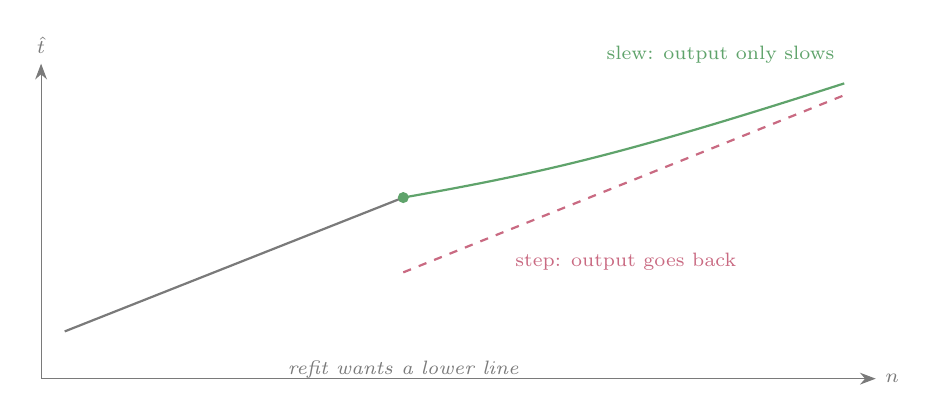
\begin{tikzpicture}[x=1cm,y=1cm]
\draw[-{Stealth[length=2mm]}, dgray] (0,0) -- (10.6,0) node[right, tag] {$n$};
\draw[-{Stealth[length=2mm]}, dgray] (0,0) -- (0,4.0) node[above, tag] {$\hat t$};
% original line
\draw[dgray, thick] (0.3,0.6) -- (4.6,2.3);
\fill[dgreen] (4.6,2.3) circle (2pt);
% step (dashed, goes back)
\draw[dashed, dpink, thick] (4.6,1.35) -- (10.2,3.6);
\node[tag, text=dpink, anchor=north west] at (5.9,1.72) {step: output goes back};
% slew (green)
\draw[dgreen, thick] (4.6,2.3) .. controls (6.4,2.62) and (7.4,2.85) .. (10.2,3.75);
\node[tag, text=dgreen, anchor=south east] at (10.2,3.88) {slew: output only slows};
\node[note, anchor=north] at (4.6,0.35) {refit wants a lower line};
\end{tikzpicture}
\caption{A refit that wants to move the line down. Applied as a step (dashed),
the next timestamp is earlier than the last one handed out. Applied through the
slew limit (green), the line bends down gradually while the index keeps
advancing, and the output stays monotone.}
\label{fig:slew}
\end{figure}

\paragraph{Monotone guard.} \code{indexToTime} still never emits a time earlier
than the newest one already emitted,
$\hat t \leftarrow \max(\hat t, t_{\text{last}})$, and counts such pulls in
\code{nMonotoneClamped} and \code{worstMonotoneClampSec}. With the slew limit in
place the count on a healthy session is zero or a handful; hundreds means the
line stepped.

\subsubsection{States of the map, and the refit algorithm}

Figure~\ref{fig:states} summarises the four states the map passes through, and
Algorithm~\ref{alg:refit} is the refit itself. The algorithm runs once per
accepted observation, after at least \code{minObs} observations are held. Lines
1--6 decide whether the window has earned the right to replace the seed slope:
the span test on line 2 is Eq.~\eqref{eq:slope}'s condition, and the clamp on
line~3 bounds how far a fit may travel from the rig-confirmed seed. Lines 7--9
compute the residuals about the OLS line and lower the intercept onto their
10th percentile, which is Eq.~\eqref{eq:offset}. Lines 10--13 are the slew
limit: the move is evaluated at the newest index, because that is where the
next sample will be stamped, and the intercept absorbs whatever part of the
move exceeds the limit. Line~14 commits both parameters together, so the map
is never left with a new slope and an old intercept.

\begin{figure}[htbp]
\centering
\resizebox{\textwidth}{!}{%
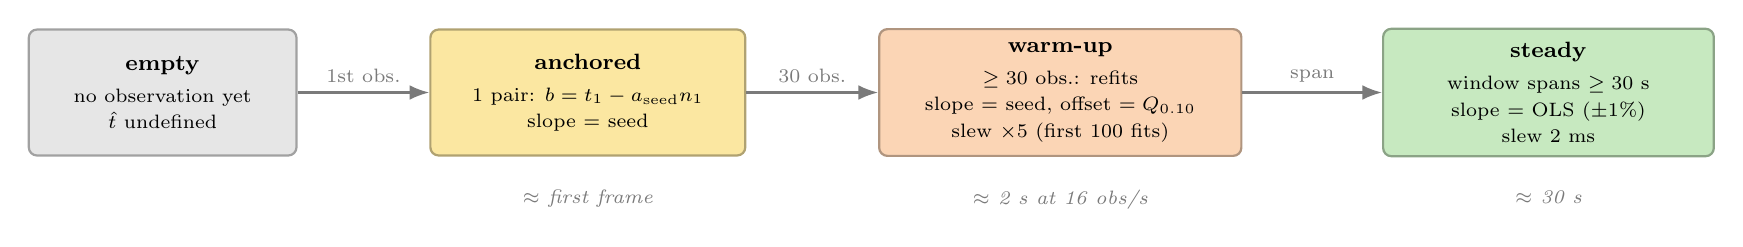
\begin{tikzpicture}
\node[blk=pgray,   minimum width=34mm, minimum height=16mm] (s0) at (0.0,0)  {\textbf{empty}\\[2pt]\scriptsize no observation yet\\\scriptsize $\hat t$ undefined};
\node[blk=pyellow, minimum width=40mm, minimum height=16mm] (s1) at (5.4,0)  {\textbf{anchored}\\[2pt]\scriptsize 1 pair: $b = t_1 - a_{\text{seed}} n_1$\\\scriptsize slope $=$ seed};
\node[blk=porange, minimum width=46mm, minimum height=16mm] (s2) at (11.4,0) {\textbf{warm-up}\\[2pt]\scriptsize $\ge 30$ obs.: refits\\\scriptsize slope $=$ seed, offset $= Q_{0.10}$\\\scriptsize slew $\times 5$ (first 100 fits)};
\node[blk=pgreen,  minimum width=42mm, minimum height=16mm] (s3) at (17.6,0) {\textbf{steady}\\[2pt]\scriptsize window spans $\ge 30$ s\\\scriptsize slope $=$ OLS ($\pm 1\%$)\\\scriptsize slew 2 ms};
\draw[lane] (s0) -- node[tag, above]{1st obs.} (s1);
\draw[lane] (s1) -- node[tag, above]{30 obs.} (s2);
\draw[lane] (s2) -- node[tag, above]{span} (s3);
\node[note, below=3mm of s1] {$\approx$ first frame};
\node[note, below=3mm of s2] {$\approx$ 2 s at 16 obs/s};
\node[note, below=3mm of s3] {$\approx$ 30 s};
\end{tikzpicture}}
\caption{States of \code{RZ2ClockMap}. Timings are for this link, which yields
about 16 accepted observations per second (roughly one drain in four arrives
empty at 60 fps with the relay at 44 Hz).}
\label{fig:states}
\end{figure}

\begin{algorithm}[htbp]
\SetAlgoLined
\DontPrintSemicolon
\KwIn{ring of accepted observations $(x_d, y_d) = (n^{(d)}, t^{(d)})$, count $n \ge$ \code{minObs}}
$x \leftarrow$ indices in window, $y \leftarrow$ arrival times; $\bar x, \bar y$ their means\;
\If{$\max x - \min x \;\ge\; 30\,\mathrm{s} \cdot f_s^{\text{seed}}$}{
  $a \leftarrow \sum (x-\bar x)(y-\bar y) \big/ \sum (x-\bar x)^2$;
  clamp $a$ to $[0.99,\,1.01]/f_s^{\text{seed}}$\;
}
\Else{
  $a \leftarrow a_{\text{current}}$ \tcp*{seed until the window has span}
}
$b \leftarrow \bar y - a\bar x$; \quad $r \leftarrow y - (b + a x)$\;
$r_Q \leftarrow$ 10th percentile of the most recent 100 entries of $r$\;
$b_{\text{new}} \leftarrow b + r_Q$\;
$m \leftarrow (b_{\text{new}} + a\,x_{\text{newest}}) - (b_{\text{old}} + a_{\text{old}} x_{\text{newest}})$\;
$s \leftarrow 2$ ms \quad ($\times 5$ during the first 100 fits)\;
\If{$|m| > s$}{
  $b_{\text{new}} \leftarrow b_{\text{new}} - \big(m - \operatorname{sign}(m)\,s\big)$\;
}
$(a_{\text{current}}, b_{\text{current}}) \leftarrow (a, b_{\text{new}})$\;
\caption{\code{RZ2ClockMap.refit()}, run after each accepted observation.}
\label{alg:refit}
\end{algorithm}

Figure~\ref{fig:scatter} shows what the estimator sees: a cloud of observations
that all sit \emph{above} the true line by their transport latency, from which
OLS recovers the slope while the intercept is lowered onto the fast tail.

\begin{figure}[htbp]
\centering
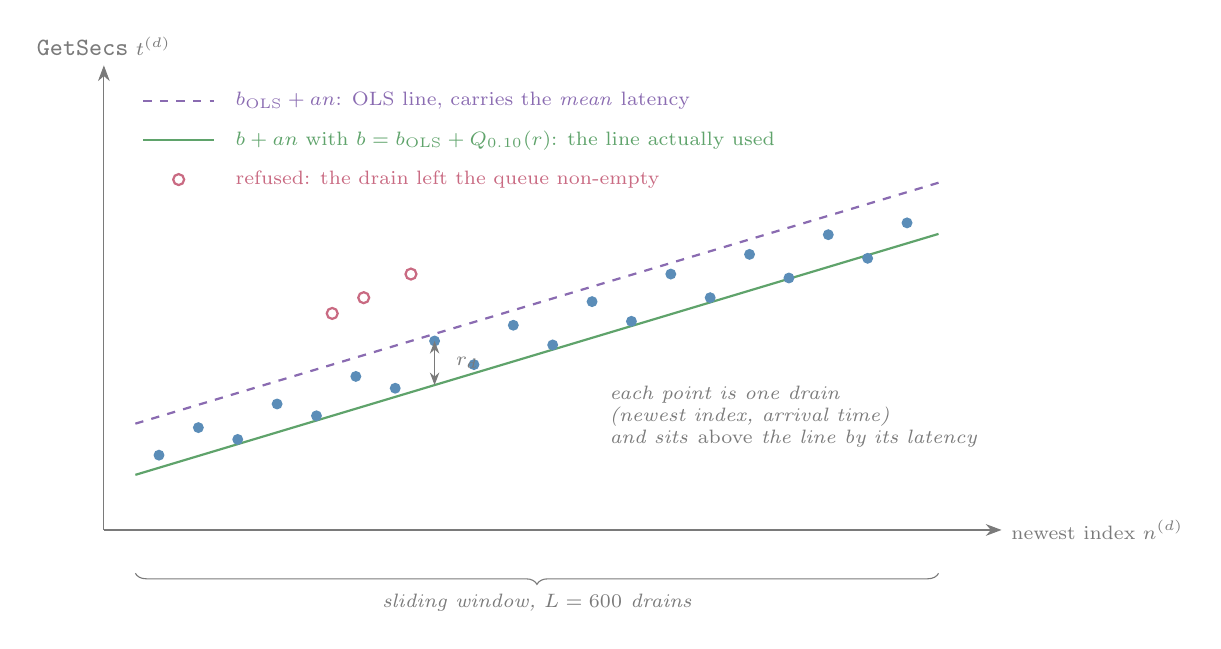
\begin{tikzpicture}[x=1cm,y=1cm]
\draw[-{Stealth[length=2mm]}, dgray] (0,0) -- (11.4,0) node[right, tag] {newest index $n^{(d)}$};
\draw[-{Stealth[length=2mm]}, dgray] (0,0) -- (0,5.9) node[above, tag] {\code{GetSecs} $t^{(d)}$};
% --- the two lines -----------------------------------------------------
\draw[dpurple, thick, dashed] (0.4,1.35) -- (10.6,4.41);
\draw[dgreen, thick]          (0.4,0.70) -- (10.6,3.76);
% --- accepted observations --------------------------------------------
\foreach \x/\y in {0.7/0.95,1.2/1.3,1.7/1.15,2.2/1.6,2.7/1.45,3.2/1.95,3.7/1.8,
                   4.2/2.4,4.7/2.1,5.2/2.6,5.7/2.35,6.2/2.9,6.7/2.65,7.2/3.25,
                   7.7/2.95,8.2/3.5,8.7/3.2,9.2/3.75,9.7/3.45,10.2/3.9}
  {\node[pt] at (\x,\y) {};}
% --- refused observations ---------------------------------------------
\foreach \x/\y in {2.9/2.75,3.3/2.95,3.9/3.25}
  {\node[circle, draw=dpink, fill=white, thick, inner sep=1.4pt] at (\x,\y) {};}
% --- residual bracket --------------------------------------------------
\draw[{Stealth[length=1.6mm]}-{Stealth[length=1.6mm]}, dgray] (4.2,1.84) -- (4.2,2.40)
      node[midway, right=1.5mm, tag] {$r_d$};
% --- legend, in the empty upper-left corner ----------------------------
\draw[dpurple, thick, dashed] (0.5,5.45) -- (1.4,5.45);
\node[tag, anchor=west, text=dpurple] at (1.55,5.45) {$b_{\mathrm{OLS}} + a n$: OLS line, carries the \emph{mean} latency};
\draw[dgreen, thick] (0.5,4.95) -- (1.4,4.95);
\node[tag, anchor=west, text=dgreen] at (1.55,4.95) {$b + a n$ with $b = b_{\mathrm{OLS}} + Q_{0.10}(r)$: the line actually used};
\node[circle, draw=dpink, fill=white, thick, inner sep=1.4pt] at (0.95,4.45) {};
\node[tag, anchor=west, text=dpink] at (1.55,4.45) {refused: the drain left the queue non-empty};
% --- note --------------------------------------------------------------
\node[note, anchor=north west, align=left] at (6.3,1.95)
      {each point is one drain\\(newest index, arrival time)\\and sits \emph{above} the line by its latency};
\draw[decorate, decoration={brace, amplitude=4pt, mirror}, dgray]
      (0.4,-0.55) -- (10.6,-0.55)
      node[midway, below=4pt, note] {sliding window, $L = 600$ drains};
\end{tikzpicture}
\caption{The affine clock map, Eq.~\eqref{eq:affine}. Observations sit above the
true line by their transport latency; OLS recovers the slope, and the intercept
is lowered to a low quantile of the residuals (10th percentile over the last
100 drains) so that only the floor latency remains as an offset. Drains that
left the queue non-empty are refused, because a trending latency would bend the
slope (Eq.~\eqref{eq:gate}).}
\label{fig:scatter}
\end{figure}

\paragraph{Implementation.} \file{ReadRZ2Joystick.m} feeds one observation per
drain and asks the map for every indexed sample's time. The order of the four
lines below is load-bearing: the backlog must be read \emph{before} the
timestamping, because it is what decides whether this drain's pair may enter the
estimator at all.

\begin{lstlisting}[language=Matlab]
backlog = u.pending();                              % RZ2Link.m; read BEFORE timestamping
rz2.clock.addObservation(iiNew(end), t2, backlog == 0);   % newest index, t2, gate
tOut(haveIdx) = rz2.clock.indexToTime(idx(haveIdx));      % affine map, monotone-guarded
ud.batch = [ud.batch; [tOut, rows(:,2), rows(:,3), idx]]; % [time, vx, vy, absIdx]
\end{lstlisting}

\file{SetupRZ2Joystick.m} constructs the map with the eight parameters of
\S\ref{sec:params-online}; \code{[]} in the fourth position leaves
\code{minObs} at its default of 30:

\begin{lstlisting}[language=Matlab]
'clock', RZ2ClockMap(OrgGet(orgParams, 'rz2SampleRateHz',        939.0024), ...
                     OrgGet(orgParams, 'rz2ClockWindow',              600), ...
                     OrgGet(orgParams, 'rz2ClockMaxRateDev',         0.01), ...
                     [], ...
                     OrgGet(orgParams, 'rz2ClockOffsetQuantile',     0.10), ...
                     OrgGet(orgParams, 'rz2ClockMaxSlewSec',        0.002), ...
                     OrgGet(orgParams, 'rz2ClockOffsetWindow',        100), ...
                     OrgGet(orgParams, 'rz2ClockMinSpanSec',           30))
\end{lstlisting}

\paragraph{Samples without an index.} Legacy-format samples (no index) fall back
to the estimate $t_j = t_1 + (t_2 - t_1)\,j/m_{\text{legacy}}$, spread evenly
across the drain interval. They are counted in \code{nLegacyFmt} and exported
with \code{RZ2Idx} $=$ \code{NaN}. Because the map now lives in the
\code{GetSecs} frame, legacy and indexed samples share one reference, so a
legacy sample dropped into a batch can no longer produce a backward step of the
accumulated divergence.

\paragraph{What the map does not fix.} The floor one-way latency is invisible
from Computer~2: a link uniformly 8~ms slow is indistinguishable from one that
is not. It stays in $b$ as a constant, cancels in every within-trial
difference, and shifts every stimulus-to-response interval by that fixed
amount. Measuring it needs a hardware loopback.

\paragraph{$f_s$ is a seed, not a divisor.} The constant only seeds $a_0$ and
centres the clamp. A wrong seed costs a warm-up of tens of drains instead of a
whole session. A Synapse \code{downsample} reset to 1 (write rate
$\sim\!24$~kHz) is far outside the $\pm 1\%$ clamp, so the slope clamps, the
skew grows, and the monitor of \S\ref{sec:skew} stops the run within a few
frames. Confirm the value on the rig with \code{getSamplingRates} and the live
\code{downsample}; do not infer it from another gizmo's displayed storage rate.

% ---------------------------------------------------------------------
\subsection{Runtime clock-skew guard}
\label{sec:skew}
% ---------------------------------------------------------------------

Every frame holds two readings of the same instant: \code{sampleTime}
(\code{GetSecs} at the cursor read) and \code{trigTime} (the timestamp of the
trajectory row that read produced, \S\ref{sec:writepaths}). On the mouse and
USB-joystick paths they are the same number by construction. On the
\code{rz2adc} path \code{trigTime} comes from the clock map, so
\begin{equation}
  \varsigma_k = \code{sampleTime}_k - \code{trigTime}_k
  \label{eq:skew}
\end{equation}
is a direct per-frame measurement of the newest sample's age (queue depth plus
any map error).

\file{ClockSkewMonitor.m} applies three rules over two statistics:

\begin{enumerate}[leftmargin=*,itemsep=2pt]
\item A throttled warning (at most one every \code{warnPeriodSec} $=5$~s) when
the \emph{instantaneous} $|\varsigma_k| \ge \code{rz2SkewWarnSec} = 0.05$~s.
\item A latching trip when the \emph{median of the last}
\code{rz2SkewWindowFrames} $= 90$ frames ($\approx 1.5$~s) reaches
\code{rz2SkewAbortSec} $= 0.20$~s. A median over 1.5~s is what a single stalled
frame cannot fake and a persistent backlog cannot hide from; tripping on one
frame killed a session for a transient stall.
\item A latching trip on a sustained run of \emph{non-finite} skew readings.
\code{indexToTime} returns \code{NaN} until the map anchors, and the map only
anchors on a drain that left the queue clear. If the queue never clears for the
whole session, every \code{trigTime} is \code{NaN}, $\varsigma_k$ is \code{NaN}
every frame, and a monitor that simply returned on a non-finite value would see
nothing to warn about while every timestamp was invalid. The threshold is
\code{nonFiniteAbortRun} $= 10 \times$ \code{windowLen} $= 900$ frames
($\approx 15$~s), long enough to cover ordinary startup before the first
observation lands.
\end{enumerate}

On a trip, \file{CenterOutTask.m} sets \code{exitFlag} and
\code{abortedByClock}, so the end-of-session text distinguishes a clock fault
from an operator abort, from a completed quota, and from a session that ran out
of stimuli. Figure~\ref{fig:monitor} shows why the median is the right statistic
for the abort.

\begin{figure}[htbp]
\centering
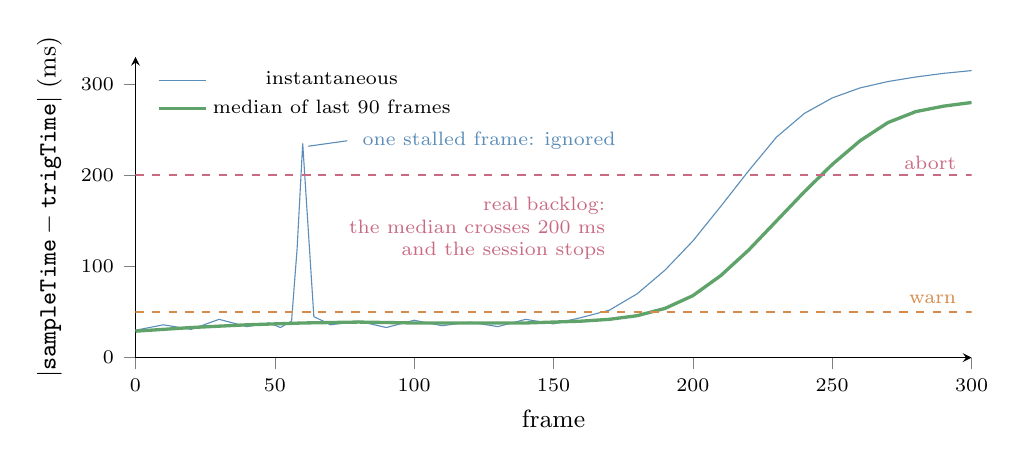
\begin{tikzpicture}
\begin{axis}[
  width=12.2cm, height=5.4cm,
  xlabel={frame}, ylabel={$|\code{sampleTime}-\code{trigTime}|$ (ms)},
  xmin=0, xmax=300, ymin=0, ymax=330,
  axis lines=left, tick align=outside,
  every axis x label/.style={at={(ticklabel cs:0.5)}, anchor=near ticklabel, font=\small},
  every axis y label/.style={at={(ticklabel cs:0.5)}, rotate=90, anchor=near ticklabel, font=\small},
  legend style={draw=none, font=\scriptsize, at={(0.015,0.99)}, anchor=north west},
  tick label style={font=\scriptsize},
]
% instantaneous: baseline 30-45, spike at 60, ramp from 170
\addplot[dblue, thin] coordinates {
 (0,30)(10,36)(20,31)(30,42)(40,34)(48,38)(52,33)(56,40)(58,120)(60,235)(62,140)
 (64,45)(70,36)(80,40)(90,33)(100,41)(110,35)(120,39)(130,34)(140,42)(150,37)
 (160,44)(170,52)(180,70)(190,96)(200,128)(210,166)(220,205)(230,242)(240,268)
 (250,285)(260,296)(270,303)(280,308)(290,312)(300,315)};
\addlegendentry{instantaneous}
% median of last 90
\addplot[dgreen, very thick] coordinates {
 (0,29)(20,33)(40,36)(60,38)(80,39)(100,38)(120,38)(140,38)(160,40)(170,42)
 (180,46)(190,54)(200,68)(210,90)(220,118)(230,150)(240,182)(250,212)(260,238)
 (270,258)(280,270)(290,276)(300,280)};
\addlegendentry{median of last 90 frames}
\addplot[dpink, dashed, thick, domain=0:300] {200};
\addplot[dorange, dashed, domain=0:300] {50};
\node[tag, text=dpink, anchor=east] at (axis cs:298,214) {abort};
\node[tag, text=dorange, anchor=east] at (axis cs:298,64) {warn};
\draw[dblue] (axis cs:62,232) -- (axis cs:76,238);
\node[tag, text=dblue, anchor=west, align=left] at (axis cs:78,238) {one stalled frame: ignored};
\node[tag, text=dpink, anchor=east, align=right] at (axis cs:172,142)
      {real backlog:\\the median crosses 200 ms\\and the session stops};
\end{axis}
\end{tikzpicture}
\caption{\code{ClockSkewMonitor}. A single spike (frame 60) never reaches the
abort line because the median does not follow it; a genuine, growing backlog
(from frame 170) does, and the session stops when the median crosses 200~ms.}
\label{fig:monitor}
\end{figure}

% ---------------------------------------------------------------------
\subsection{One clock per comparison}
\label{sec:oneclock}
% ---------------------------------------------------------------------

With the sample clock corrected, one structural rule remains: the state machine
must never compare a capture time against a wall-clock time inside a single
expression. Every window anchored on a cursor event (\code{t.centerHold},
\code{t.leaveCenter}, \code{t.reachTarget}, \code{t.holdStart} in
\file{CenterOutTask.m}, and \code{t.centerHold}, \code{t.targetHit} in
\file{CenterInTask.m}) is tested against \code{trigTime}, not \code{this\_time}.

Let $T_\ell$ and $T_r$ be the capture times of leaving the centre and reaching
the target, and $L$ the transport latency. Then
\begin{align}
  \text{old:}\quad & \underbrace{T_r + L}_{\text{wall now}} \le T_\ell + D
    &&\iff\quad T_r - T_\ell \le D - L, \label{eq:oldrule}\\
  \text{new:}\quad & \underbrace{T_r}_{\code{trigTime}} \le T_\ell + D
    &&\iff\quad T_r - T_\ell \le D. \label{eq:newrule}
\end{align}
The latency cancels. The decision window is anchored on the stimulus flip (wall
clock, from \code{Screen('AsyncFlipEnd')}'s \code{StimulusOnsetTime}) and tested
against \code{trigTime} as well: that is the true reaction time up to the link's
constant floor latency, instead of reaction time plus the queue. The honest side
effect is that during a stall \code{trigTime} does not advance, so a hold takes
the stall longer to confirm; without samples there is nothing to confirm it
with. On mouse and USB input \code{trigTime} equals \code{sampleTime} and
nothing changes. Figure~\ref{fig:oneclock} shows both rules on the same trial.

\begin{figure}[htbp]
\centering
\resizebox{0.96\textwidth}{!}{%
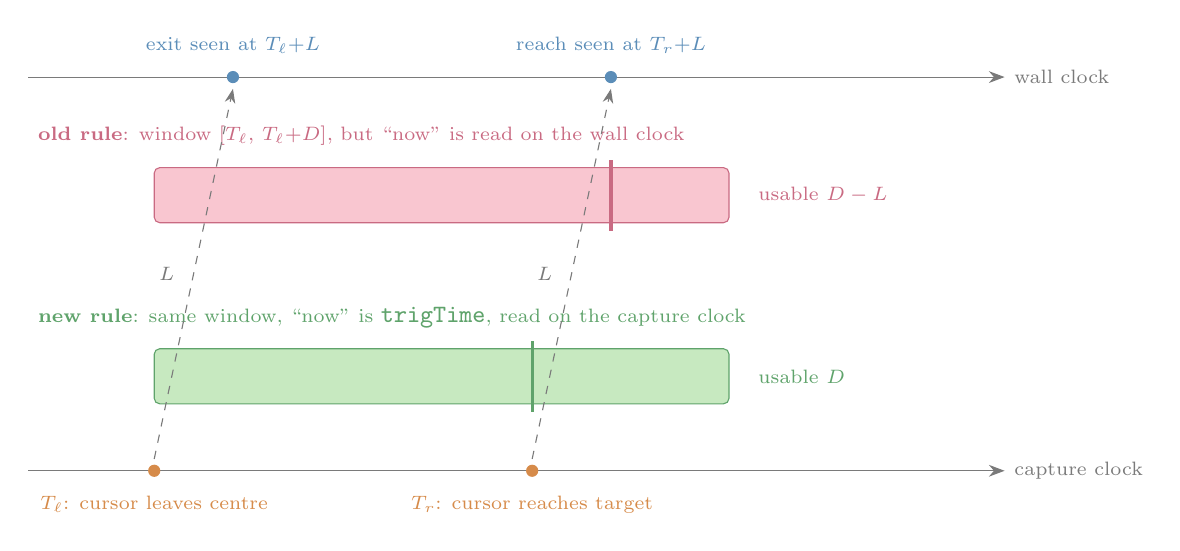
\begin{tikzpicture}[x=1cm,y=1cm]
% ---- wall clock -----------------------------------------------------
\draw[-{Stealth[length=2mm]}, dgray] (0,0) -- (12.4,0) node[right, tag] {wall clock};
\fill[dblue] (2.6,0) circle (2.2pt);
\node[tag, text=dblue, anchor=south] at (2.6,0.18) {exit seen at $T_\ell{+}L$};
\fill[dblue] (7.4,0) circle (2.2pt);
\node[tag, text=dblue, anchor=south] at (7.4,0.18) {reach seen at $T_r{+}L$};

% ---- old rule -------------------------------------------------------
\node[tag, text=dpink, anchor=west] at (0.0,-0.75)
      {\textbf{old rule}: window $[T_\ell,\,T_\ell{+}D]$, but ``now'' is read on the wall clock};
\draw[fill=ppink, draw=dpink, rounded corners=2pt] (1.6,-1.85) rectangle (8.9,-1.15);
\draw[dpink, very thick] (7.4,-1.95) -- (7.4,-1.05);
\node[tag, text=dpink, anchor=west] at (9.15,-1.5) {usable $D-L$};

% ---- new rule -------------------------------------------------------
\node[tag, text=dgreen, anchor=west] at (0.0,-3.05)
      {\textbf{new rule}: same window, ``now'' is \code{trigTime}, read on the capture clock};
\draw[fill=pgreen, draw=dgreen, rounded corners=2pt] (1.6,-4.15) rectangle (8.9,-3.45);
\draw[dgreen, very thick] (6.4,-4.25) -- (6.4,-3.35);
\node[tag, text=dgreen, anchor=west] at (9.15,-3.8) {usable $D$};

% ---- capture clock --------------------------------------------------
\draw[-{Stealth[length=2mm]}, dgray] (0,-5.0) -- (12.4,-5.0) node[right, tag] {capture clock};
\fill[dorange] (1.6,-5.0) circle (2.2pt);
\node[tag, text=dorange, anchor=north] at (1.6,-5.2) {$T_\ell$: cursor leaves centre};
\fill[dorange] (6.4,-5.0) circle (2.2pt);
\node[tag, text=dorange, anchor=north] at (6.4,-5.2) {$T_r$: cursor reaches target};

% ---- latency arrows -------------------------------------------------
\foreach \s/\d in {1.6/2.6, 6.4/7.4} {
  \draw[dashed, dgray, -{Stealth[length=1.8mm]}] (\s,-4.85) -- (\d,-0.15);
  \node[tag, text=dgray, anchor=east] at ($(\s,-4.85)!0.5!(\d,-0.15) + (-0.12,0)$) {$L$};
}
\end{tikzpicture}}
\caption{One clock per comparison. The window (the coloured band) is the same in
both rules; only the ``now'' it is tested against changes, marked by the
vertical bar. Reading ``now'' on the capture clock removes $L$ from the
inequality entirely.}
\label{fig:oneclock}
\end{figure}

The two rules appear in the code as:

\begin{lstlisting}[language=Matlab]
% CenterOutTask.m, EP.MOVEMENT
withinWindow = trigTime <= t.leaveCenter + maxExecutionTime;
% CenterOutTask.m, EP.HOLD
if trigTime > t.centerHold + holdTime && inCenterCircle
% CenterOutTask.m, EP.DECISION_TIME
if trigTime <= t.targetOnset + maxDecisionTime
\end{lstlisting}

\noindent
The first line bounds the movement window: both ends are capture times, so the
window is exactly \code{maxExecutionTime} long. The second confirms the centre
hold from the capture clock and the position of the same row, so a hold is
confirmed by samples rather than by elapsed wall time. The third anchors the
decision window on \code{t.targetOnset}, which is the flip's
\code{StimulusOnsetTime} and therefore a wall-clock instant, and tests it against
\code{trigTime}: that mixture is deliberate, because the stimulus really did
appear at a wall-clock instant and the response really was observed on the
capture clock, so their difference is the reaction time plus the link's constant
floor latency and nothing else.

Stimulus-driven windows that do not depend on the cursor (\code{cueDuration},
\code{barToTargetDelay}, the bar and ITI durations) stay on \code{this\_time}:
they measure how long something was on the screen, which is a wall-clock
quantity.

\paragraph{The cached row.} A frame that drained nothing writes a
cached-position row (write path 2, \S\ref{sec:writepaths}). Under one clock per
comparison, stamping it with \code{sampleTime} would make \code{trigTime} jump
ahead of the stream by the link's latency on every such frame. The row inherits
the \emph{previous row's} time instead: ``now'' in capture time, when nothing
new has arrived, is the time of the newest sample that exists. Before the first
sample of the session there is no capture clock yet, so the wall clock stands in.

% ---------------------------------------------------------------------
\subsection{Gap accounting}
% ---------------------------------------------------------------------

Let $n^{(1)} < n^{(2)} < \dots$ be the indices seen across drains, including the
seam with the previous drain (\code{ud.lastIdx}). The number of missing samples
is
\begin{equation}
  N_{\text{skipped}} \;=\; \sum_k \max\!\big(n^{(k+1)} - n^{(k)} - 1,\; 0\big),
  \label{eq:skipped}
\end{equation}
accumulated in \code{ud.nSkipped}. Lost datagrams and relay recalibration jumps
both appear here and are not distinguishable from Computer~2, so they are
reported together. Gaps \emph{between} datagrams of the same drain are counted
too, not only the seam, because a single datagram lost in the middle of a busy
frame is exactly the case a seam-only check would miss. A deliberate flush by
\file{FlushRZ2Joystick.m} resets \code{lastIdx} to \code{NaN} so the discarded
backlog is not counted as loss; it goes to \code{nFlushed} instead.

% ---------------------------------------------------------------------
\subsection{Bounded drain and backlog dynamics}
\label{sec:drain}
% ---------------------------------------------------------------------

Let $M$ be the per-frame drain cap (\code{rz2MaxSamplesPerDrain} $= 2048$),
$f_{\text{fr}}$ the frame rate (60~Hz) and $B$ a backlog that has accumulated in
the socket. Each frame removes at most $M$ samples while $f_s$ new ones arrive
per second, so the backlog after $k$ frames is
\begin{equation}
  B_k = \max\!\Big(B_0 - k\big(M - f_s/f_{\text{fr}}\big),\; 0\Big),
  \qquad
  k^{\star} = \left\lceil \frac{B_0}{M - f_s/f_{\text{fr}}} \right\rceil,
  \label{eq:backlog}
\end{equation}
so a 97\,100-sample burst clears in $k^\star \approx 48$ frames
($\approx 0.8$~s) at $M = 2048$. An unbounded drain is what lets a backlog feed
on itself: the longer the queue, the longer the frame that has to swallow it,
which grows the queue further. The cap is checked \emph{before} a datagram is
read and a datagram is always consumed whole, so the true ceiling is $M$ plus
one relay cycle; capping mid-datagram would discard samples already taken off
the socket, which is strictly worse than leaving them queued. A warning is
emitted only after \code{rz2CapWarnFrames} $= 60$ consecutive capped frames
(about one second), since transient capping after any loop stall is normal and
self-clearing. The worst backlog seen and the number of capped frames are
reported at teardown.

The receive buffer must hold the burst while it drains. At roughly 29 bytes per
sample, \code{rz2InputBufferSize} $= 4\,194\,304$ bytes holds $\approx 145\,000$
samples ($\approx 154$~s at 939~Hz), comfortably above the largest burst seen.

% ---------------------------------------------------------------------
\subsection{Flush before the loop starts}
% ---------------------------------------------------------------------

\file{FlushRZ2Joystick.m} discards whatever queued between socket open and
trial-loop start. The setup steps and the modal recording checklist
(\file{ConfirmRecordingLink.m}) can take many seconds, i.e.\ thousands of
samples, and those samples describe a period the task was not running: they are
backlog, not data. The function resets \code{batch}, \code{lastIdx},
\code{capConsec} and \code{lastDrainTime}, and returns the number of datagrams
(or bytes, on the legacy transport) discarded.

The clock map is deliberately left alone. Its observations are (index, arrival)
pairs, and discarding queued datagrams removes future observations without
invalidating any past one; re-anchoring here would introduce exactly the
discontinuity the flush exists to avoid, and the session stays on one timeline.
A stale first observation is no longer fatal in any case (it is one of $L$ and
is eventually refitted away), but flushing still avoids seconds of capped frames
at the start of the session.

% ---------------------------------------------------------------------
\subsection{Transport selection}
\label{sec:link}
% ---------------------------------------------------------------------

\file{RZ2Link.m} owns the socket and hides which transport is in use behind one
API: \code{readOne()}, \code{pending()}, \code{flush()}, \code{close()},
\code{describe()}. It tries three transports in order and keeps the first that
opens:

\begin{enumerate}[leftmargin=*,itemsep=2pt]
\item \textbf{\code{java.nio.channels.DatagramChannel}, non-blocking}
(\code{mode = 'java'}). This is what the rig uses. A non-blocking channel has no
helper thread: \code{receive()} returns immediately with a datagram if the
operating system has one and \code{null} if it does not, so the drain loop sees
the OS queue directly, at frame rate. It ships with every JRE MATLAB has
bundled. \code{pending()} cannot report a depth here and returns 0 when the last
\code{readOne} found the queue empty and 1 otherwise, which is exactly the
boolean the clock map's gate needs.
\item \textbf{\code{udpport}} (MATLAB R2019b and later),
\code{pending()} $=$ datagrams available.
\item \textbf{Legacy \code{udp()}}, with \code{InputBufferSize} and
\code{InputDatagramPacketSize} applied; \code{pending()} $=$ bytes available.
\end{enumerate}

The rig's Computer~2 runs MATLAB R2016b, so \code{udpport} is unavailable and
the legacy object was the transport until the NIO channel replaced it. The
legacy object delivers datagrams through a Java helper thread that fills
\code{BytesAvailable} on its own schedule, and on this rig that schedule is
coarse: with the relay sending every $\approx 23$~ms, a third of the 67~ms
drain windows came back empty, which is impossible under direct delivery
(three relay cycles fit in one window). Datagrams were being handed over in
clumps, and waiting for the next clump was most of the measured sample age. A
transient Java exception on the non-blocking receive (for example an ICMP
port-unreachable when the relay bounces) is counted in \code{nReadErrors} and
treated as an empty read, because it is recoverable on the next frame and must
not abort a session. The mode actually opened is printed at startup and again at
teardown.

% =====================================================================
\section{How the two joysticks are read}
\label{sec:read}
% =====================================================================

The task accepts three input sources, selected by \code{orgParams.inputSource}
(\code{'joystick'} $|$ \code{'mouse'} $|$ \code{'rz2adc'}). The two joysticks
differ in every respect that matters for a trajectory: where they are sampled,
at what rate, who timestamps them, and how many rows per frame they produce.
Table~\ref{tab:paths} summarises; the subsections give the mechanics.

\begin{table}[htbp]
\centering
\small
\begin{tabular}{@{}P{3.0cm}P{5.4cm}P{6.5cm}@{}}
\toprule
 & USB joystick (\code{'joystick'}) & RZ2 analog joystick (\code{'rz2adc'}) \\
\midrule
Transducer read by & Computer 2, \code{vrjoystick(1)} (Simulink 3D Animation) &
  PZ5 amplifier $\rightarrow$ RZ2 processor, TDT Synapse on Computer 1 \\[2pt]
Sample rate & Two reads per rendered frame (base $+$ one oversample 8~ms
  later), $\approx 120$~Hz; HID native $\approx 125$~Hz &
  $f_s \approx 939$~Hz per axis, independent of the frame rate \\[2pt]
Native units & Axes already in $[-1,1]$ (driver) &
  Volts, normalised to $[-1,1]$ by \code{JOY\_RANGE} $= 4.6$~V on Computer 1 \\[2pt]
Timestamp & \code{GetSecs} at the read (\code{sampleTime}); exact by
  construction & Relay sample index $n_i$ mapped through \code{RZ2ClockMap}
  into the \code{GetSecs} frame \\[2pt]
Rows per frame & 2 & All samples drained that frame, typically 15--17 \\[2pt]
Latency & USB polling interval, sub-frame (4--10~ms) &
  Relay period $+$ UDP $+$ queue depth; measured per frame as $\varsigma_k$ \\[2pt]
Clocks in play & one & two, reconciled by \code{RZ2ClockMap} (\S\ref{sec:clock}) \\[2pt]
Can drift & no & only if the rate were a fixed constant, which it is not \\[2pt]
Runtime guard & none needed & \code{ClockSkewMonitor} (\S\ref{sec:skew}) \\[2pt]
Provenance column & \code{RZ2Idx} $=$ \code{NaN} & \code{RZ2Idx} $= n_i$ \\[2pt]
Gain / offset & \code{joyGain} ($-1.3$), \code{pointer\_offset} &
  \code{rz2ScaleX}, \code{rz2ScaleY} (1, 1), \code{rz2OffsetY} (0) \\
\bottomrule
\end{tabular}
\caption{The two joystick paths side by side.}
\label{tab:paths}
\end{table}

% ---------------------------------------------------------------------
\subsection{USB joystick: polled once per frame on Computer 2}
% ---------------------------------------------------------------------

\file{SetupJoystick.m} opens the device once, \code{joy = vrjoystick(1)}, and
fails with an explicit error if index 1 is not a recognised joystick. Each frame
\file{ReadCursorPosition.m} does:

\begin{lstlisting}[language=Matlab]
axesVals = read(joy);                          % [ax1, ax2, ...] in [-1, 1]
x = xCenter + screenXpixels * axesVals(1, 1) * joyGain;
y = yCenter + pointer_offset + screenYpixels * axesVals(1, 2) * joyGain;
\end{lstlisting}

\noindent
so the sampling process is the frame loop itself: the joystick is a function
$\bm{u}(t)$ observed at the frame instants $t_k$, with $t_{k+1} - t_k \approx
1/60$~s and jitter equal to the loop's own jitter. There is no buffer, no index
and no queue; the timestamp written to \code{trajBuf} is the same \code{GetSecs}
the state machine uses, so the skew of \S\ref{sec:skew} is identically zero and
the monitor is not run on this path.

The oversample loop (\code{moveOversample} $= 1$, \code{moveOversampleDt} $=
0.008$~s) takes one extra read while the asynchronous flip is pending. It is
skipped entirely on the \code{rz2adc} path, where the batch write already logs
every sample the relay delivered and a second read would only re-drain an
already-drained socket. The 8~ms spacing is this rig's measured HID update
interval ($\approx 125$~Hz), so two reads per frame is the most the device can
deliver without duplicating cached values; the effective rate is therefore
$\approx 120$ samples/s, close to the 125~Hz grid of \S\ref{sec:offline}, and
the Savitzky--Golay window of 11 grid samples spans roughly 11 real reads. One
extra read is used rather than several because at $\approx 8$~ms per sample,
three extra reads would span 24~ms, longer than a 16.7~ms frame, and the burst
would run past the vsync it is supposed to be free inside of.

On this path \code{trigTime} is literally \code{sampleTime}, so every comparison
in the state machine was already on one clock and \S\ref{sec:oneclock} changes
nothing; \code{Time\_ms} is non-decreasing by construction, and there is no rate
to get wrong, no anchor, no window and no monitor.

% ---------------------------------------------------------------------
\subsection{RZ2 joystick, Computer 1 side: Synapse ring buffer and relay}
\label{sec:c1}
% ---------------------------------------------------------------------

\paragraph{Signal path in Synapse.} The joystick's two analog outputs enter the
PZ5, which streams to the RZ2 at the TDT base rate
$f_{\text{base}} = 24414.0625$~Hz. Two \code{APIStreamer1Ch.rcx} gizmos,
\code{APICh1X} and \code{APICh2Y}, decimate by \code{downsample} $= D = 26$ and
write into a \code{SerStore} ring buffer of $B = \code{BUF\_SIZE} = 100\,000$
samples each:
\begin{equation}
  f_s = \frac{f_{\text{base}}}{D} = \frac{24414.0625}{26} = 939.0024 \ \text{Hz},
  \qquad
  \text{ring capacity} = \frac{B}{f_s} \approx 106.5 \ \text{s}.
  \label{eq:fs}
\end{equation}
Each gizmo exposes a write-index tag (surfacing through SynapseAPI under the
literal name \code{'???'}, the tag having reached the API without a resolved
label), the position $W \in [0, B)$ of the next sample to be written.

\paragraph{Relay cycle.} The relay (\file{StepJoystickRelay.m}) is stepped from
the \file{categTaskCommunication} GUI loop and is a no-op until
\code{RELAY\_PERIOD} $= 1/169.4$~s has elapsed. In write-index mode
(\code{WRITE\_IDX\_TAG\_X/Y} non-empty, the configuration on this rig) one cycle
is:

\begin{enumerate}[leftmargin=*,itemsep=1pt]
\item Read the write heads $W_x, W_y$ through \code{getParameterValue}, reduced
modulo $B$.
\item Compute the signed circular distance from the read cursor $C$ to the head,
\begin{equation}
  \Delta(W, C) = \big((W - C) \bmod B\big) - B\,\big[(W - C) \bmod B > B/2\big],
  \label{eq:circdelta}
\end{equation}
(\code{circDelta}: the representative of $W-C$ in $(-B/2, B/2]$). A negative
value means the head was read behind the cursor, which is jitter or pacing that
outran the writer; it is counted in \code{nHeadBehind} and clamped to 0. The
unsigned version, \code{circDist}, discards the sign on purpose for its
tolerance check, which is why the signed variant had to be introduced
separately.
\item Read $n = \min(\Delta_x, \Delta_y, \code{MAX\_READ\_PER\_CYCLE} = 4096)$
samples from each ring at offset $C$, in two pieces if the window wraps past $B$
(\code{readBufWindow}), and advance $C \leftarrow (C + n) \bmod B$.
\item Normalise and clip, $v = \operatorname{clip}(\text{raw}/\code{JOY\_RANGE},
-1, 1)$, with \code{JOY\_RANGE} $= 4.6$~V.
\item Attach absolute indices $n_i = N_{\text{abs}}, N_{\text{abs}}+1, \dots$
(the running count \code{absIdx}, never reduced modulo $B$) and send them as
datagrams of at most \code{MAX\_SAMPLES\_PER\_DGRAM} $= 17$ lines, formatted
column-major by a single \code{sprintf} with
\code{'N:\%.0f,X:\%.4f,Y:\%.4f\textbackslash n'}.
\item $N_{\text{abs}} \leftarrow N_{\text{abs}} + n_{\text{done}}$, where
$n_{\text{done}}$ is how far the read cursors \emph{actually} advanced this
cycle: $n$ when both buffer reads succeeded, 0 if either threw. Advancing by
$n$ unconditionally, outside the \code{try}, while the cursors advanced inside
it, meant a failed read re-sent the same samples under new indices.
\end{enumerate}

Healthy steady state is $n \approx f_s/169.4 \approx 5.5$ samples per cycle,
i.e.\ about 169 datagrams per second on the wire (two per cycle since the
per-datagram cap went to 17). After any stall on Computer~1 the backlog is read
in bursts of up to 4096 samples, split into datagrams of 17.
Figure~\ref{fig:ring} shows the two cursors on the ring.

\begin{figure}[htbp]
\centering
\resizebox{0.98\textwidth}{!}{%
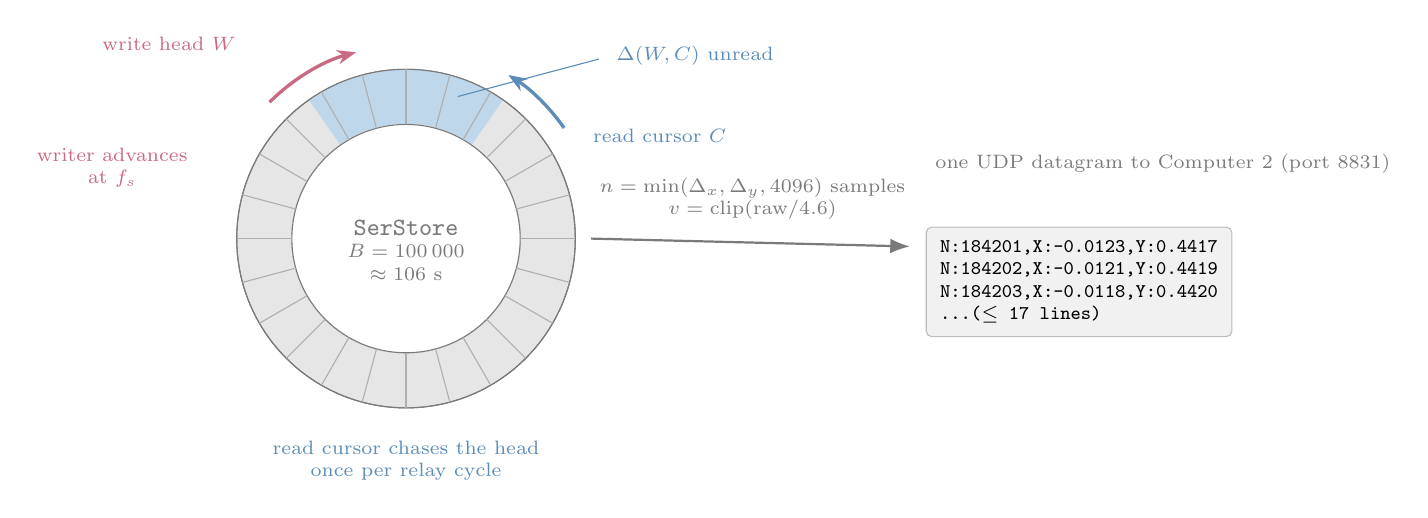
\begin{tikzpicture}[x=1cm,y=1cm]
% ring
\draw[fill=pgray, draw=dgray] (0,0) circle (2.15);
\draw[fill=white, draw=dgray] (0,0) circle (1.45);
% unread arc
\begin{scope}
  \clip (0,0) circle (2.15);
  \fill[pblue] (0,0) -- (55:2.3) arc (55:125:2.3) -- cycle;
  \draw[white] (0,0) circle (1.45);
  \fill[white] (0,0) circle (1.45);
\end{scope}
\draw[dgray] (0,0) circle (2.15);
\draw[dgray] (0,0) circle (1.45);
% ticks
\foreach \a in {0,15,...,345} {\draw[dgray!60] (\a:1.45) -- (\a:2.15);}
% heads
\draw[-{Stealth[length=2.4mm]}, dpink, very thick] (135:2.45) arc (135:105:2.45);
\node[tag, text=dpink, anchor=south east] at (132:3.05) {write head $W$};
\draw[-{Stealth[length=2.4mm]}, dblue, very thick] (35:2.45) arc (35:58:2.45);
\node[tag, text=dblue, anchor=west] at (30:2.6) {read cursor $C$};
\draw[dblue] (2.45,2.28) -- (70:1.92);
\node[tag, text=dblue, anchor=west] at (2.55,2.32) {$\Delta(W,C)$ unread};
\node[tag, align=center] at (0,-0.15) {\code{SerStore}\\$B = 100\,000$\\$\approx 106$ s};
\node[tag, text=dpink, anchor=east, align=center] at (-2.65,0.9) {writer advances\\at $f_s$};
\node[tag, text=dblue, anchor=north, align=center] at (0,-2.45) {read cursor chases the head\\once per relay cycle};
% datagram box
\node[draw=dgray!50, fill=codebg, rounded corners=2pt, inner sep=5pt,
      font=\ttfamily\scriptsize, align=left, anchor=west] (dg) at (6.6,-0.55)
  {N:184201,X:-0.0123,Y:0.4417\\
   N:184202,X:-0.0121,Y:0.4419\\
   N:184203,X:-0.0118,Y:0.4420\\
   ...($\le$ 17 lines)};
\node[tag, anchor=west] at (6.6,0.95) {one UDP datagram to Computer 2 (port 8831)};
\draw[lane] (2.35,0.0) -- (6.4,-0.1);
\node[tag, anchor=south, align=center] at (4.4,0.12)
  {$n = \min(\Delta_x,\Delta_y,4096)$ samples\\$v = \operatorname{clip}(\text{raw}/4.6)$};
\end{tikzpicture}}
\caption{Relay cycle on Computer 1: both cursors move counter-clockwise, the
writer at $f_s$, the read cursor in jumps of $n$ once per cycle. The shaded arc
is what is still unread, and it is what gets normalised, indexed with the
running \code{absIdx}, and pushed over UDP.}
\label{fig:ring}
\end{figure}

\paragraph{Datagram size.} Both machines use the legacy \code{udp()} object on
the send side, whose \code{OutputDatagramPacketSize} defaults to 512 bytes and
truncates anything larger. At 26--27 bytes per sample, 40 samples per datagram
is $\approx 630$ bytes and every datagram was cut at byte 512. The cap is now
\code{MAX\_SAMPLES\_PER\_DGRAM} $= 17$ ($17 \times 30$ bytes worst case
$= 510 < 512$), and the packet-size properties on both sides were raised to
8192 as a second lock.

\paragraph{Cost per SynapseAPI call.} Every \code{getParameterValue} is an HTTP
round trip of $\approx 5$~ms regardless of payload, so four calls per cycle pin
the loop at $\approx 44$~Hz against a 169.4~Hz target. The Y write index is
therefore read only every \code{IDX\_Y\_CHECK\_EVERY} $= 10$ cycles: X and Y
advance in lockstep by construction, the relay already takes their minimum, and
a check that finds them more than \code{IDX\_Y\_TOL} $= 2$ samples apart warns
once and reverts to reading both every cycle. Three calls instead of four is
$\approx 17$~ms per cycle. Getting to two would need X and Y interleaved in one
\code{.rcx} buffer, which is a circuit change.

\paragraph{Legacy fallback, and the startup check that makes it reachable.} If
the write-index tags cannot be read, the relay paces itself by time,
$n = \operatorname{round}(\code{READ\_FS} \cdot \Delta t_{\text{cycle}})$ with
$\code{READ\_FS} = \code{N\_READ} \times \code{RELAY\_HZ} = 6 \times 169.4 =
1016.4$~Hz, and to re-synchronise every \code{RECAL\_INTERVAL\_SEC} $= 10$~s by
the diff-peak method: two snapshots of a \code{RECAL\_WINDOW} $= 6000$-sample
window separated by \code{CALIBRATION\_WAIT\_SEC} $= 0.15$~s, with the head
located at $\arg\max_j \big(|d_2 - d_1| * \tfrac{1}{100}\bm{1}_{100}\big)_j$
(\file{ActiveIndexFromSnapshots.m}).

How this path is entered is the part that changed. Reading a tag is not what
detects a bad tag: SynapseAPI's \code{getParameterValue} and
\code{getParameterValues} do not throw for a nonexistent name, so \code{idxOk}
inside \code{readWriteIndex()} can never go false from a wrong
\code{WRITE\_IDX\_TAG\_X/Y}, \code{widxFellBack} never fires, and the relay
would anchor to whatever the call returned and then read zero new samples for
the rest of the session without a warning. \file{InitJoystickRelay.m} therefore
checks existence once, at startup, immediately after the two tag names are set:
\code{getParameterNames} is called on \code{APICh1X} and \code{APICh2Y} and each
name is looked up case-insensitively in the list it returns. If either is
absent, a warning names the missing tag and its gizmo, both fields are reset to
the empty string, and the session runs on the legacy path, which is exactly what
the empty-string convention already meant. \code{getParameterNames} rather than
\code{getParameterInfo} because \file{VerifyWidxWidy.m} found that
\code{getParameterInfo} can fail on tags that do exist, which makes it a
diagnostic and not a test; \code{getParameterNames} is what
\file{ProbeJoystickBuffers.m} and \file{VerifyWidxWidy.m} already use to prove a
tag is real.

The check is at startup and not per cycle on purpose. A
\code{getParameterNames} round trip inside \code{readWriteIndex()} would put a
fourth HTTP call back into a loop whose cost is measured and logged, to catch a
tag that disappears mid-session, which is not a failure this rig has produced.
What remains true of the legacy path is that \code{WRITE\_FS} $= 1017$,
\code{READ\_FS} and the recalibration constants were tuned against a write rate
that was never real, so the fallback is now reachable but still mis-tuned; it is
a loud degradation rather than a silent freeze, not a second correct mode. On
this rig the question is hypothetical: \code{WRITE\_IDX\_TAG\_X/Y} are
\code{'???'} and have been readable since 2026-08-25, so the check exists for
the next repointing.

\paragraph{\code{WRITE\_FS} $= 1017$ is still active in the diagnostics.} It no
longer drives the read, but it feeds two things an operator is told to watch:
the ``$\sim X$~ms behind head'' line of the 5-second log, which divides the
backlog by 1017 and therefore reads 7.7\,\% low against 939~Hz, and
\file{VerifyWidxWidy.m}'s \code{ASSUMED\_FS} $= 1017$, which would report a
7.7\,\% deviation from a link that is behaving perfectly. The maintainers'
stated plan is not to paste 939 in but to have \file{InitJoystickRelay.m}
measure the rate at relay startup, as Computer~2 now does, keeping the constant
as seed and sanity bound; that yields two independent estimates of the same
quantity, one per machine, whose disagreement is itself a diagnostic.

% ---------------------------------------------------------------------
\subsection{RZ2 joystick, Computer 2 side: listen, drain, time, log}
% ---------------------------------------------------------------------

Computer 2 only listens. \file{SetupRZ2Joystick.m} opens port 8831 through
\file{RZ2Link.m} (\S\ref{sec:link}), which selects the transport at startup and
prints which one it opened. \code{UserData} lives on the \file{RZ2Link} handle
in every mode, so \code{rz2.port.UserData} is unchanged for the rest of the
code, and a channel left open by a crashed session is closed on the next open.
Per frame:

\begin{enumerate}[leftmargin=*,itemsep=2pt]
\item \file{ReadCursorPosition.m} calls \file{ReadRZ2Joystick.m}, which drains
up to $M$ samples (\S\ref{sec:drain}), feeds the clock map one observation,
times every sample through Eq.~\eqref{eq:affine}, appends
$[t_i, v_{x,i}, v_{y,i}, n_i]$ to \code{UserData.batch}, and returns only the
newest $(v_x, v_y)$ for rendering and hit-testing.
\item \file{CenterOutTask.m} calls \file{TakeRZ2JoystickSamples.m}, which pops
the whole batch and clears it, and writes one trajectory row per sample
(\S\ref{sec:writepaths}). The pop is a separate function from the drain so the
socket is drained exactly once per frame (inside the render read) while the full
batch is still available for logging.
\item The state machine acts on the newest row; the skew monitor compares its
timestamp to \code{sampleTime} (\S\ref{sec:skew}).
\end{enumerate}

Figure~\ref{fig:twopaths} compares the two input paths and
Figure~\ref{fig:oneframe} shows what one frame contributes on each.

\begin{figure}[htbp]
\centering
\resizebox{\textwidth}{!}{%
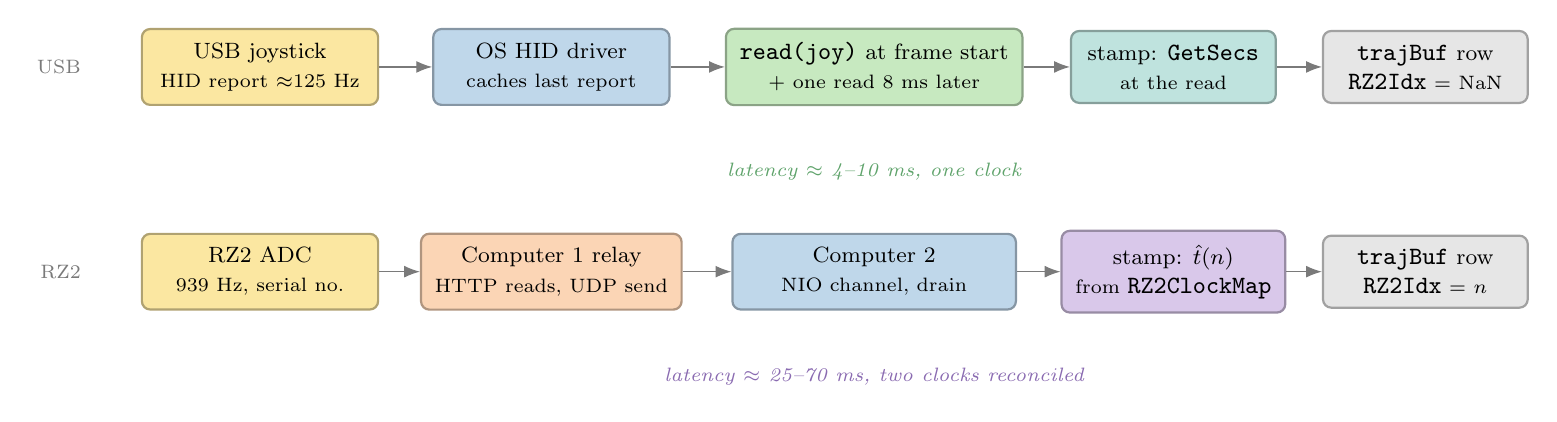
\begin{tikzpicture}
% USB row
\node[tag, anchor=east] at (-0.35,0) {USB};
\node[blk=pyellow, minimum width=30mm] (u1) at (1.8,0)  {USB joystick\\[1pt]\scriptsize HID report $\approx$125 Hz};
\node[blk=pblue,   minimum width=30mm] (u2) at (5.5,0)  {OS HID driver\\[1pt]\scriptsize caches last report};
\node[blk=pgreen,  minimum width=36mm] (u3) at (9.6,0)  {\code{read(joy)} at frame start\\[1pt]\scriptsize $+$ one read 8 ms later};
\node[blk=pteal,   minimum width=26mm] (u4) at (13.4,0) {stamp: \code{GetSecs}\\[1pt]\scriptsize at the read};
\node[blk=pgray,   minimum width=26mm] (u5) at (16.6,0) {\code{trajBuf} row\\[1pt]\scriptsize \code{RZ2Idx} = NaN};
\foreach \a/\b in {u1/u2,u2/u3,u3/u4,u4/u5} {\draw[thin lane] (\a) -- (\b);}
\node[note, text=dgreen, below=6mm of u3] {latency $\approx$ 4--10 ms, one clock};

% RZ2 row
\node[tag, anchor=east] at (-0.35,-2.6) {RZ2};
\node[blk=pyellow, minimum width=30mm] (r1) at (1.8,-2.6)  {RZ2 ADC\\[1pt]\scriptsize 939 Hz, serial no.};
\node[blk=porange, minimum width=30mm] (r2) at (5.5,-2.6)  {Computer 1 relay\\[1pt]\scriptsize HTTP reads, UDP send};
\node[blk=pblue,   minimum width=36mm] (r3) at (9.6,-2.6)  {Computer 2\\[1pt]\scriptsize NIO channel, drain};
\node[blk=ppurple, minimum width=26mm] (r4) at (13.4,-2.6) {stamp: $\hat t(n)$\\[1pt]\scriptsize from \code{RZ2ClockMap}};
\node[blk=pgray,   minimum width=26mm] (r5) at (16.6,-2.6) {\code{trajBuf} row\\[1pt]\scriptsize \code{RZ2Idx} = $n$};
\foreach \a/\b in {r1/r2,r2/r3,r3/r4,r4/r5} {\draw[thin lane] (\a) -- (\b);}
\node[note, text=dpurple, below=6mm of r3] {latency $\approx$ 25--70 ms, two clocks reconciled};
\end{tikzpicture}}
\caption{The two input paths side by side. The USB path has one machine and one
clock; the stamp is the wall clock at the moment of the read. The RZ2 path has
two machines, a serial number per sample, and an estimator that maps serial
numbers back onto Computer 2's clock. The point of the exercise is the last row
of Table~\ref{tab:paths}: the RZ2 path is harder because its samples are on the
same clock as the neural recording.}
\label{fig:twopaths}
\end{figure}

\begin{figure}[htbp]
\centering
\resizebox{\textwidth}{!}{%
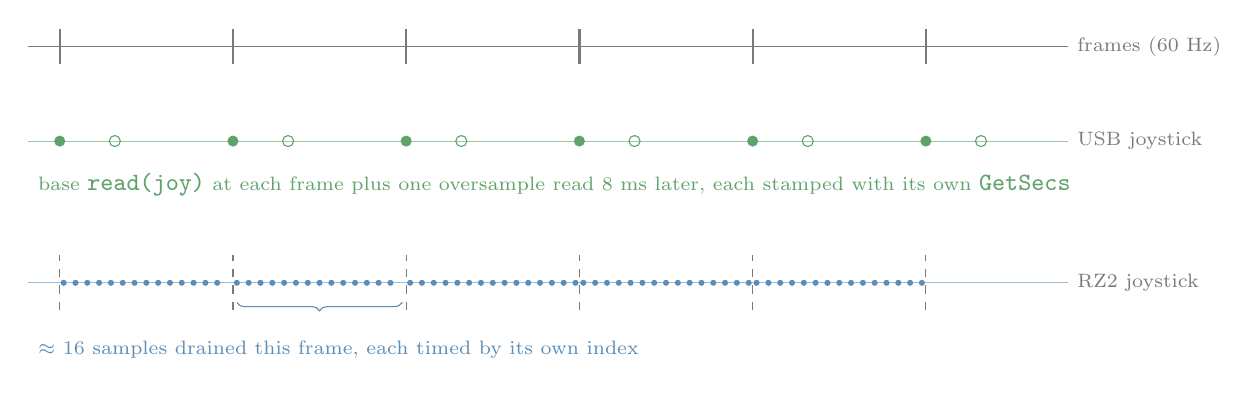
\begin{tikzpicture}[x=1cm,y=1cm]
% frames
\draw[dgray] (0,0) -- (13.2,0) node[right, tag] {frames (60 Hz)};
\foreach \x in {0.4,2.6,...,11.6} {\draw[dgray, thick] (\x,-0.22) -- (\x,0.22);}
% USB
\draw[dgreen!60] (0,-1.2) -- (13.2,-1.2) node[right, tag] {USB joystick};
\foreach \x in {0.4,2.6,...,11.6} {\fill[dgreen] (\x,-1.2) circle (2pt);}
\foreach \x in {1.1,3.3,...,12.3} {\draw[dgreen] (\x,-1.2) circle (2pt);}
\node[tag, text=dgreen, anchor=west, align=left] at (0.0,-1.75)
  {base \code{read(joy)} at each frame plus one oversample read 8 ms later, each stamped with its own \code{GetSecs}};
% RZ2
\draw[dblue!60] (0,-3.0) -- (13.2,-3.0) node[right, tag] {RZ2 joystick};
\foreach \x in {0.4,2.6,...,11.6} {\draw[dashed, dgray] (\x,-3.35) -- (\x,-2.65);}
\foreach \x in {0.45,0.6,...,2.55} {\fill[dblue] (\x,-3.0) circle (1.1pt);}
\foreach \x in {2.65,2.8,...,4.75} {\fill[dblue] (\x,-3.0) circle (1.1pt);}
\foreach \x in {4.85,5.0,...,6.95} {\fill[dblue] (\x,-3.0) circle (1.1pt);}
\foreach \x in {7.05,7.2,...,9.15} {\fill[dblue] (\x,-3.0) circle (1.1pt);}
\foreach \x in {9.25,9.4,...,11.35} {\fill[dblue] (\x,-3.0) circle (1.1pt);}
\draw[decorate, decoration={brace, amplitude=3pt, mirror}, dblue] (2.65,-3.25) -- (4.75,-3.25);
\node[tag, text=dblue, anchor=west] at (0.0,-3.85)
  {$\approx$ 16 samples drained this frame, each timed by its own index};
\end{tikzpicture}}
\caption{What one frame contributes to the trajectory on each path.}
\label{fig:oneframe}
\end{figure}

\paragraph{Resolution.} The relay writes four decimals in $[-1,1]$, so the
smallest representable step is $10^{-4}$ in normalised units, i.e.
$4.6 \times 10^{-4}$~V. Through Eq.~\eqref{eq:map} this maps to
$W s_x \times 10^{-4} = 0.19$~px horizontally and
$H s_y \times 10^{-4} = 0.11$~px vertically at unit gain: the wire format is not
the limiting quantisation. The USB path's resolution is whatever the HID driver
reports (commonly 8--10 bits per axis, i.e.\ 5--20~px at $|\code{joyGain}| =
1.3$), which is one reason the Hampel stage's $\mathrm{MAD} = 0$ guard
(\S\ref{sec:hampel}) fires more often on that path.

% =====================================================================
\section{Screen mapping and hit testing}
\label{sec:screen}
% =====================================================================

% ---------------------------------------------------------------------
\subsection{Affine map from joystick units to pixels}
% ---------------------------------------------------------------------

For the \code{rz2adc} input source (\file{ReadCursorPosition.m} and the batch
loop in \file{CenterOutTask.m}):
\begin{equation}
  x_i = x_c + W s_x v_{x,i},
  \qquad
  y_i = y_c + o_y + H s_y v_{y,i}.
  \label{eq:map}
\end{equation}
The map is affine and axis-separable; $s_x, s_y$ carry both magnitude (pixels
per unit deflection, as a fraction of the screen extent) and sign (axis
inversion). For the USB joystick the same form is used with
$s_x = s_y = \code{joyGain}$ (default $-1.3$) and $o_y =
\code{pointer\_offset}$. Mouse mode reads pixels directly.

Because Eq.~\eqref{eq:map} is applied identically to the rendered sample and to
every logged batch sample, the CSV columns \code{X\_px} and \code{Y\_px} are
exactly the pixel coordinates the state machine saw. The inverse map recovers
joystick units offline if needed:
$v_x = (x - x_c)/(W s_x)$, $v_y = (y - y_c - o_y)/(H s_y)$.

% ---------------------------------------------------------------------
\subsection{Circular acceptance regions}
% ---------------------------------------------------------------------

Both the centre hold window and the targets are drawn as discs and tested as
discs. Given a Psychtoolbox rect $[x_1, y_1, x_2, y_2]$,
\begin{equation}
  c_x = \frac{x_1 + x_2}{2}, \quad
  c_y = \frac{y_1 + y_2}{2}, \quad
  r   = \frac{x_2 - x_1}{2},
  \qquad
  \text{inside} \iff (x - c_x)^2 + (y - c_y)^2 \le r^2 .
  \label{eq:circle}
\end{equation}
\file{CheckInCircle.m} takes $(c_x, c_y)$ and the left and right edges;
\file{CheckInTargetCenterOut.m} takes the full rect and returns false for an
unplaced (all-zero) rect. Both are exact, with no dependence on frame rate or
hardware.

Figure~\ref{fig:geometry} shows the geometry and how the epoch tags follow from
these tests. The hit tests on each sample are what convert a continuous path
into the \code{DECISION\_TIME} / \code{MOVEMENT} / \code{TARGET\_HOLD} labels in
the trajectory file. The \code{MOVEMENT} epoch is the one that measures the
\emph{execution time}, \code{t.reachTarget} $-$ \code{t.leaveCenter}, which is
what \code{ExecutionTime\_s} carries in \code{trial\_data\_*.csv}; the figure
is labelled with that name, and \code{MOVEMENT} (code 7) is the identifier the
code and the \code{Epoch} column use for it.

\begin{figure}[htbp]
\centering
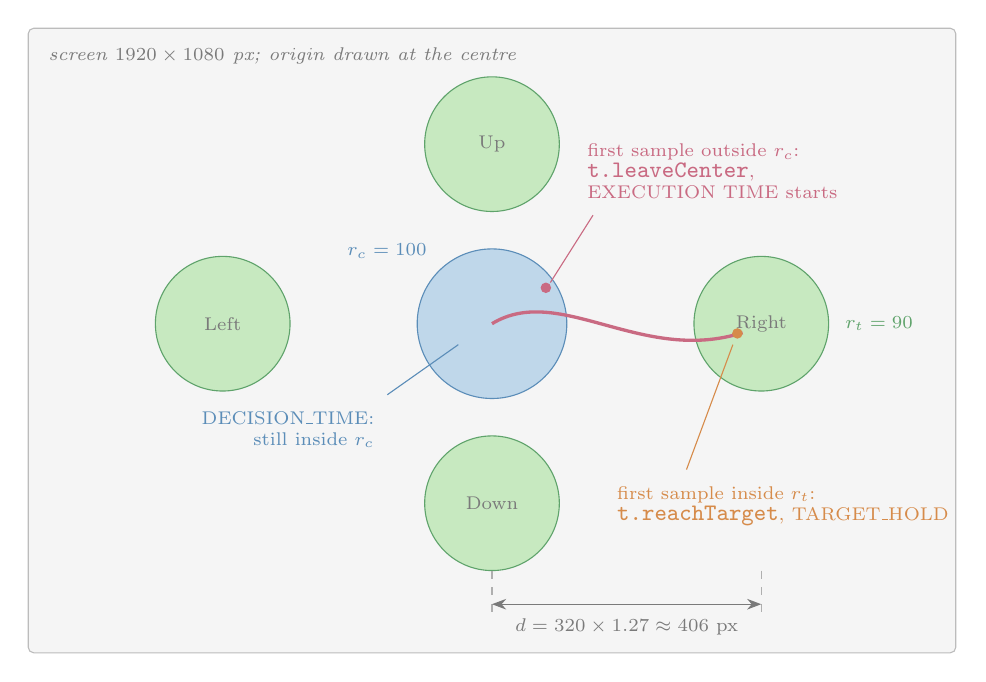
\begin{tikzpicture}[x=1cm,y=1cm, scale=0.95, every node/.style={transform shape}]
\draw[fill=pgray!40, draw=dgray!50, rounded corners=2pt] (-6.2,-4.4) rectangle (6.2,3.95);
\node[note, anchor=north west] at (-6.05,3.82) {screen $1920 \times 1080$ px; origin drawn at the centre};
% centre
\draw[fill=pblue, draw=dblue] (0,0) circle (1.0);
\node[tag, text=dblue, anchor=south east] at (-0.75,0.75) {$r_c = 100$};
% targets
\draw[fill=pgreen, draw=dgreen] (3.6,0) circle (0.9) node[tag] {Right};
\draw[fill=pgreen, draw=dgreen] (0,2.4) circle (0.9) node[tag] {Up};
\draw[fill=pgreen, draw=dgreen] (-3.6,0) circle (0.9) node[tag] {Left};
\draw[fill=pgreen, draw=dgreen] (0,-2.4) circle (0.9) node[tag] {Down};
\node[tag, text=dgreen, anchor=west] at (4.6,0.0) {$r_t = 90$};
% path
\draw[dpink, very thick] (0,0) .. controls (0.9,0.55) and (2.0,-0.55) .. (3.35,-0.12);
\fill[dpink] (0.72,0.48) circle (2pt);
\fill[dorange] (3.28,-0.13) circle (2pt);
\node[tag, text=dpink, anchor=south west, align=left] at (1.15,1.55)
  {first sample outside $r_c$:\\\code{t.leaveCenter},\\EXECUTION TIME starts};
\draw[dpink] (0.78,0.55) -- (1.35,1.45);
\node[tag, text=dorange, anchor=north west, align=left] at (1.55,-2.05)
  {first sample inside $r_t$:\\\code{t.reachTarget}, TARGET\_HOLD};
\draw[dorange] (3.22,-0.28) -- (2.6,-1.95);
\node[tag, text=dblue, anchor=north east, align=right] at (-1.45,-1.05)
  {DECISION\_TIME:\\still inside $r_c$};
\draw[dblue] (-1.4,-0.95) -- (-0.45,-0.28);
% distance
\draw[dgray!60, dashed] (0,-3.30) -- (0,-3.85);
\draw[dgray!60, dashed] (3.6,-3.30) -- (3.6,-3.85);
\draw[{Stealth[length=1.8mm]}-{Stealth[length=1.8mm]}, dgray] (0,-3.75) -- (3.6,-3.75);
\node[tag, anchor=north] at (1.8,-3.82) {$d = 320 \times 1.27 \approx 406$ px};
\end{tikzpicture}
\caption{Geometry used by the hit tests, Eq.~\eqref{eq:circle}, and how the
epochs follow from them. The interval that opens at \code{t.leaveCenter} and
closes at \code{t.reachTarget} is the execution time; its epoch code is
\code{MOVEMENT} $= 7$. Distances come from the session's own
\code{params\_<runTag>.mat} when the notebook reads it (\S\ref{sec:reading});
the task reads its own values from the console.}
\label{fig:geometry}
\end{figure}

% =====================================================================
\section{Trajectory buffer and export}
\label{sec:buffer}
% =====================================================================

% ---------------------------------------------------------------------
\subsection{Buffer layout}
% ---------------------------------------------------------------------

Every logged sample is one row of $\code{trajBuf} \in \mathbb{R}^{N \times 9}$
in \file{CenterOutTask.m} (and $N \times 7$ in \file{CenterInTask.m}, which has
no Block or TrialNumInBlock columns):
\begin{equation}
  \big[\ \text{TrialNum},\ \tau,\ x,\ y,\ \text{Epoch},\ \text{Block},\
  \text{TrialNumInBlock},\ \text{Attempt},\ \text{RZ2Idx}\ \big],
  \label{eq:row}
\end{equation}
with
\begin{equation}
  \tau = \max\!\big(1000\,(\hat t_i - T_0),\, 0\big).
  \label{eq:tau}
\end{equation}

\code{RZ2Idx} is the relay's absolute sample index $n_i$ for rows the RZ2 batch
wrote, and \code{NaN} for every other row (USB, mouse, oversample, empty-batch
cached rows, legacy-format samples). It is the row's provenance flag:
\code{NaN} means the time is estimated rather than index-derived, and it lets an
offline analysis re-derive timing under a different clock model without
re-running anything (\S\ref{sec:offlineclock}). The clamp at 0 exists because
the very first drained batch of a session can carry times slightly earlier than
$T_0$, and it does so on either path: an indexed sample is timed by the clock
map, a legacy index-less sample is interpolated from \code{lastDrainTime}, and
both are readings of \code{GetSecs} on a link that was already streaming from
Computer~1 before Computer~2 stamped $T_0$. The clamp writes those few rows as
exactly 0 rather than letting a trajectory open with negative times.

The buffer is preallocated at $\code{trajChunk} = 200\,000$ rows and grows in
chunks of that size (or by the batch size if larger), so no per-row
reallocation happens inside the frame loop.

\begin{figure}[htbp]
\centering
\resizebox{\textwidth}{!}{%
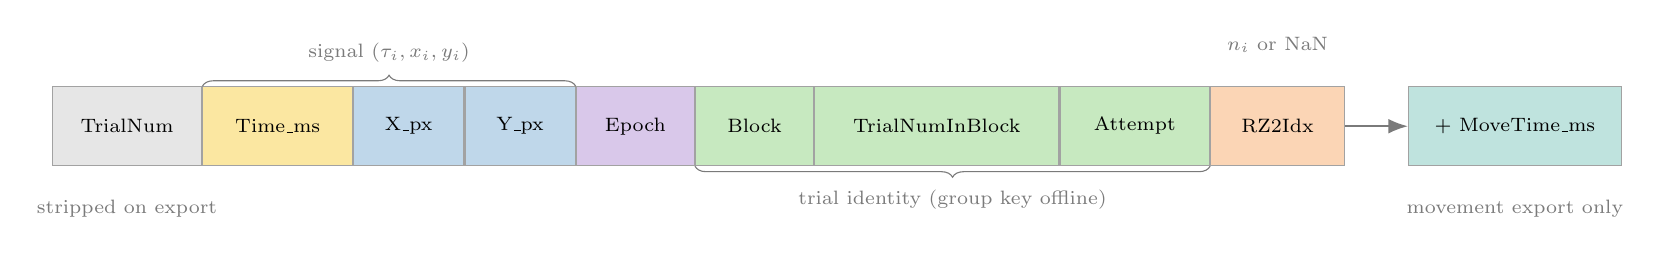
\begin{tikzpicture}[x=1cm,y=1cm,
   cell/.style={rectangle, draw=dgray!70, fill=#1, minimum height=10mm,
                align=center, font=\scriptsize, inner sep=3pt}]
% widths chosen so each label fits: cells are placed edge to edge.
\node[cell=pgray,   minimum width=19mm, anchor=west] (c1) at (0.00,0) {TrialNum};
\node[cell=pyellow, minimum width=19mm, anchor=west] (c2) at (c1.east) {Time\_ms};
\node[cell=pblue,   minimum width=14mm, anchor=west] (c3) at (c2.east) {X\_px};
\node[cell=pblue,   minimum width=14mm, anchor=west] (c4) at (c3.east) {Y\_px};
\node[cell=ppurple, minimum width=15mm, anchor=west] (c5) at (c4.east) {Epoch};
\node[cell=pgreen,  minimum width=15mm, anchor=west] (c6) at (c5.east) {Block};
\node[cell=pgreen,  minimum width=31mm, anchor=west] (c7) at (c6.east) {TrialNumInBlock};
\node[cell=pgreen,  minimum width=19mm, anchor=west] (c8) at (c7.east) {Attempt};
\node[cell=porange, minimum width=17mm, anchor=west] (c9) at (c8.east) {RZ2Idx};
\node[cell=pteal,   minimum width=27mm, anchor=west] (c10) at ([xshift=8mm]c9.east) {$+$ MoveTime\_ms};
\draw[lane] (c9.east) -- (c10.west);

% annotations
\draw[decorate, decoration={brace, amplitude=4pt}, dgray]
      (c2.north west) -- (c4.north east)
      node[midway, above=5pt, tag] {signal $(\tau_i, x_i, y_i)$};
\draw[decorate, decoration={brace, amplitude=4pt, mirror}, dgray]
      (c6.south west) -- (c8.south east)
      node[midway, below=5pt, tag] {trial identity (group key offline)};
\node[tag, anchor=north] at ([yshift=-3mm]c1.south) {stripped on export};
\node[tag, anchor=south] at ([yshift=3mm]c9.north) {$n_i$ or NaN};
\node[tag, anchor=north] at ([yshift=-3mm]c10.south) {movement export only};
\end{tikzpicture}}
\caption{Row layout of \code{trajBuf} (\file{CenterOutTask.m}) and its two
exports. \file{TrajectoryColumnNames.m} recognises the 8- and 6-column stripped
layouts (with \code{RZ2Idx}) and the older 7- and 5-column ones.}
\label{fig:rowlayout}
\end{figure}

% ---------------------------------------------------------------------
\subsection{Three write paths, one timestamp rule}
\label{sec:writepaths}
% ---------------------------------------------------------------------

Per frame the loop writes rows through one of three paths, all producing $\tau$
the same way, that is, at the instant the row's own $(x,y)$ was read:

\begin{enumerate}[leftmargin=*,itemsep=2pt]
\item \textbf{\code{rz2adc} with a non-empty batch}: one row per drained sample,
with $x, y$ from Eq.~\eqref{eq:map} applied to that sample's $(v_x, v_y)$, $\tau$
from Eq.~\eqref{eq:affine}, and \code{RZ2Idx} $= n_i$.
\item \textbf{\code{rz2adc} with an empty batch} (relay stall): one row with the
cached last position and the \emph{previous row's} $\tau$, so \code{trajN} still
advances exactly once per frame and the column stays on one clock
(\S\ref{sec:oneclock}); \code{RZ2Idx} $=$ \code{NaN} marks it as cached.
\item \textbf{USB joystick or mouse}: one row per frame, plus
\code{moveOversample} rows taken \code{moveOversampleDt} apart while the
asynchronous flip is pending; \code{RZ2Idx} $=$ \code{NaN}.
\end{enumerate}

The state machine then acts on the newest row:

\begin{lstlisting}[language=Matlab]
trigRowIdx = trajN;
trigTime   = sessionT0 + trajBuf(trigRowIdx, 2) / 1000;
\end{lstlisting}

\noindent
Reading the time back \emph{out of the row}, rather than copying it from
\code{sampleTime}, is what guarantees that \code{t.leaveCenter} and
\code{t.reachTarget} refer to the same sample the hit test used, and therefore
that \code{MoveTime\_ms} $= 0$ lands exactly on the leave-centre sample
downstream. Both \code{trigRowIdx} and \code{trigTime} are captured before the
render block, because the oversample loop reassigns \code{sampleTime} and
advances \code{trajN}: by the time the state machine runs, those would refer to
the last extra read rather than to the sample that drove the decision.

% ---------------------------------------------------------------------
\subsection{Epoch retagging at movement onset}
% ---------------------------------------------------------------------

When the cursor first leaves the centre after target onset, the rows from the
triggering sample to the current end of the buffer are retagged:

\begin{lstlisting}[language=Matlab]
trajBuf(trigRowIdx:trajN, 5) = EP.MOVEMENT.Value;
\end{lstlisting}

\noindent
so the first row carrying the \code{MOVEMENT} code (7) is the sample whose hit
test returned ``outside centre''. Without this the epoch label lands one frame
late, the first \code{MOVEMENT} row is the next frame's, and
\code{MoveTime\_ms} $= 0$ sits a frame behind \code{t.leaveCenter}. Retagging
also puts the real first point of the movement into the export, which it was
otherwise missing. Epoch codes used offline: \code{DECISION\_TIME} $= 6$,
\code{MOVEMENT} $= 7$, \code{TARGET\_HOLD} $= 8$.

% ---------------------------------------------------------------------
\subsection{Exports}
% ---------------------------------------------------------------------

\file{SaveTrajectory.m} writes the whole buffer (all epochs) with the
\code{TrialNum} column removed. The movement export
(\file{SaveMovementTrajectory.m}) keeps rows with
$\text{Epoch} \in \code{movementExportEpochs} = \{6, 7, 8\}$ and appends
\begin{equation}
  \code{MoveTime\_ms}_i \;=\; \tau_i - \min_{j \in g(i)} \tau_j,
  \label{eq:movetime}
\end{equation}
where $g(i)$ is the set of rows sharing the identity columns (Block,
TrialNumInBlock, Attempt) with row $i$. The minimum, rather than the first row,
is used because batch timestamps can land slightly out of row order, which would
otherwise make the first record's \code{MoveTime\_ms} negative and shift the
whole trial. The identity columns are those \emph{between} Epoch and
\code{RZ2Idx}: including \code{RZ2Idx} in the group key would make every row its
own group and every \code{MoveTime\_ms} exactly zero, silently, since a column
of zeros is a perfectly well-formed column.

\code{Time\_ms} is left untouched in both files, so rows can be joined across
them. Both exporters call \file{ReportTimeMonotonicity.m}, which prints the
number and worst size of backward steps in \code{Time\_ms} and otherwise stays
silent. It reports and does not repair: reordering or clamping there would hide
a live instrumentation fault behind a tidy-looking file, so a file with a
warning is one whose intervals must not be trusted where the steps occur. Both
exporters also refuse to guess a layout: the caller declares its own literal
column count (\code{expectedRawCols}, 9 for \file{CenterOutTask.m} and 7 for
\file{CenterInTask.m}), and a mismatch is treated as a save failure and recorded
by \file{WriteSaveFailureMarker.m} rather than written out.

Alongside the trajectories, \file{CenterConsole.m} writes
\code{params\_<runTag>.mat} \emph{before} the task starts: a snapshot of
\code{runTag}, session and subject identifiers, engine name, timestamp, and the
full merged \code{orgParams} struct with the non-serializable \code{handles}
field removed. A crash mid-session therefore still leaves a record of what was
configured, and the offline geometry of \S\ref{sec:reading} is read from it.

% =====================================================================
\section{Offline chain: the EDA signal-processing pipeline}
\label{sec:offline}
% =====================================================================

All offline processing lives in the section 1.1 cell of the single-session
notebook (\file{EDA\_SINGLE\_SESSION\_...ipynb}); the multi-session notebook
carries a copy of the same definitions in its section 0.2 cell, with the
per-trial figure drawer and \code{run()} left behind. The classes involved are
\code{ScreenGeometry}, \code{InputSourceDetector}, \code{HampelScreen},
\code{KalmanTrajectorySmoother}, \code{ButterworthLowpass},
\code{TrajectoryProcessor} and \code{TrajectoryDataset}, plus
\code{OfflineClockFit}, which is in the single-session notebook only
(\S\ref{sec:offlineclock}).

% ---------------------------------------------------------------------
\subsection{Reading a session: source, profile and geometry}
\label{sec:reading}
% ---------------------------------------------------------------------

Before any filter runs, \code{TrajectoryDataset.\_\_init\_\_} decides three
things about the file it has just read.

\paragraph{Input source.} \code{InputSourceDetector.detect} classifies each
trajectory file as \code{rz2adc}, \code{usb} or \code{unknown}:
\begin{equation}
  \text{source} =
  \begin{cases}
    \text{override} & \text{if the run tag matches a key of \code{INPUT\_SOURCE\_OVERRIDES}},\\
    \code{rz2adc} & \text{else if \code{RZ2Idx} has any finite value},\\
    \code{rz2adc} & \text{else if } \operatorname{median}_k(\Delta \tau_k) < \code{RZ2\_MAX\_MEDIAN\_STEP\_MS} = 3\ \text{ms},\\
    \code{usb} & \text{else if that median is finite},\\
    \code{unknown} & \text{otherwise.}
  \end{cases}
  \label{eq:detect}
\end{equation}
The median step is taken within trials (grouped by Block, TrialNumInBlock,
Attempt) over positive differences only, so it is not contaminated by the jump
between trials. The RZ2 path delivers $\approx 1.06$~ms steps and the USB path
$\approx 8$~ms, so the two are separated by a factor of eight; mouse sessions
also land in \code{usb}. The detection is printed per file and appears in every
figure title.

\paragraph{Pipeline profile.} The source selects a \code{PipelineProfile} from
\code{PIPELINE\_PROFILES}, which carries the Hampel half-window and threshold,
the Kalman measurement and jerk noise, the $\chi^2$ gate, and one boolean,
\code{drop\_unindexed\_rows}. Both profiles currently start from the same filter
values, so nothing changes until a profile is edited; the mechanism exists so
that a per-source change can be made in one place rather than by branching
inside the processor. \code{TrajectoryProcessor.for\_profile} is the only
constructor the analysis cells use.

\paragraph{Un-indexed rows.} On a session detected as \code{rz2adc}, rows whose
\code{RZ2Idx} is \code{NaN} are removed when the file is read. Those are exactly
the cached rows a frame writes when no new sample arrived (write path 2 of
\S\ref{sec:writepaths}) and any un-indexed legacy samples: rows whose position
is a repeat of the previous row's and whose time, by design since the cached row
inherits the previous row's $\tau$, is also a repeat. They carry no new
information, and dropping them removes the only rows on that path whose time is
estimated. The count is printed and kept in
\code{df.attrs["n\_unindexed\_dropped"]}. On the USB path every row has
\code{RZ2Idx} $=$ \code{NaN}, which is why the flag is off for that profile; on
an export older than the \code{RZ2Idx} column the notebook says so and keeps
every row.

\paragraph{Epoch filter.} \code{move\_epochs} is applied explicitly here rather
than trusting the CSV to already be restricted: a row is kept when its
\code{Epoch} matches any listed code. A text \code{Epoch} column (from an older
export) is mapped to numeric codes through \code{\_EPOCH\_NAME\_TO\_CODE} first,
and unrecognised names are reported rather than silently dropped. Which codes
are loaded differs by cell \emph{by design}: the section 1.1 cell loads
$(6,7,8)$ so the target hold is available for the hold flags, while the
trajectory-EDA cell and the feature table load $(6,7)$. Because the summary
window of \S\ref{sec:summary} is now bounded by target entry rather than by the
end of the loaded rows, the same trial yields the same summaries under both
choices.

\paragraph{Screen geometry.} \code{ScreenGeometry.resolve} takes the hit-test
geometry (centre and target diameters, centre-to-target distance and its scale)
from the first of these that is available:
\begin{enumerate}[leftmargin=*,itemsep=1pt]
\item \code{orgParams} inside the session's own \code{params\_<runTag>.mat}
(\code{centerRad}, \code{targetRad}, \code{centerToTargetDist}), which is the
real source of truth for the screen the task rendered that day;
\item a \code{geometry\_spec*.json} or \code{geometry\_spec*.csv} sitting next to
the session's \code{trial\_data\_*.csv}, kept as a manual override for sessions
that predate the params export (accepted layouts: a JSON object, a two-column
\code{key,value} CSV, or a one-row CSV with the keys as headers);
\item the module constants (\code{CENTER\_DIAMETER\_PX} $= 200$,
\code{TARGET\_DIAMETER\_PX} $= 180$, \code{CENTER\_TO\_TARGET\_DIST\_PX} $=
320$, \code{TARGET\_DIST\_SCALE} $= 1.27$).
\end{enumerate}
Any key missing from a file keeps its default, and the printed line names the
source and lists what fell back. The resulting target radius is what
\code{hold\_unstable} is compared against (\S\ref{sec:flags}).

% ---------------------------------------------------------------------
\subsection{Pipeline order}
% ---------------------------------------------------------------------

For one trial, with samples $(t_k, x_k, y_k)$, $k = 1, \dots, n$:

\paragraph{Pre-processing (\code{TrajectoryProcessor.process}).} Times are
converted to seconds and sorted with a stable sort; duplicate timestamps are
removed with \code{np.unique(t, return\_index=True)}, keeping the \emph{first}
occurrence, and counted in \code{n\_duplicate\_ts}. A trial is flagged
\emph{under-resolved} if $n < \code{min\_move\_samples} = 5$ (or, if
\code{min\_move\_dur\_s} is set, if its duration is below it); kinematics are
then returned as \code{NaN} but the filtered trace is still produced, so the
trial still appears in the figures with its flag.

\begin{figure}[htbp]
\centering
\resizebox{\textwidth}{!}{%
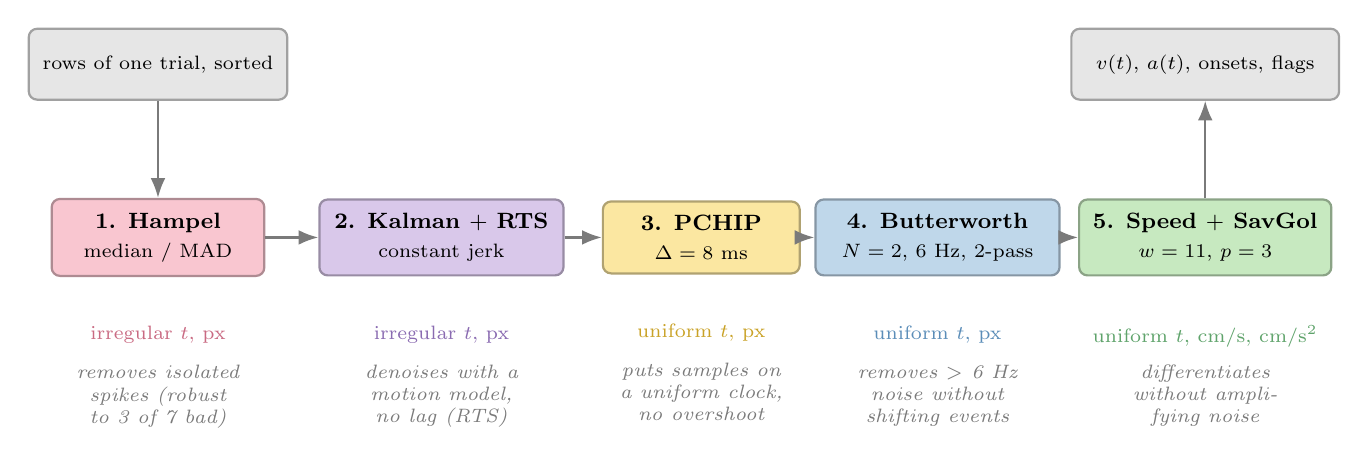
\begin{tikzpicture}
\node[blk=pgray, minimum width=30mm] (in) at (0,2.2) {\scriptsize rows of one trial, sorted};
\node[blk=ppink,   minimum width=27mm] (s1) at (0.0,0)  {\textbf{1. Hampel}\\[1pt]\scriptsize median / MAD};
\node[blk=ppurple, minimum width=31mm] (s2) at (3.6,0)  {\textbf{2. Kalman $+$ RTS}\\[1pt]\scriptsize constant jerk};
\node[blk=pyellow, minimum width=25mm] (s3) at (6.9,0)  {\textbf{3. PCHIP}\\[1pt]\scriptsize $\Delta = 8$ ms};
\node[blk=pblue,   minimum width=31mm] (s4) at (9.9,0)  {\textbf{4. Butterworth}\\[1pt]\scriptsize $N=2$, 6 Hz, 2-pass};
\node[blk=pgreen,  minimum width=31mm] (s5) at (13.3,0) {\textbf{5. Speed $+$ SavGol}\\[1pt]\scriptsize $w=11$, $p=3$};
\node[blk=pgray,   minimum width=34mm] (out) at (13.3,2.2) {\scriptsize $v(t)$, $a(t)$, onsets, flags};
\foreach \a/\b in {s1/s2,s2/s3,s3/s4,s4/s5} {\draw[lane] (\a) -- (\b);}
\draw[lane] (in.south) -- (s1.north);
\draw[lane] (s5.north) -- (out.south);
% time base row
\node[tag, text=dpink,   below=5mm of s1] {irregular $t$, px};
\node[tag, text=dpurple, below=5mm of s2] {irregular $t$, px};
\node[tag, text=dyellow, below=5mm of s3] {uniform $t$, px};
\node[tag, text=dblue,   below=5mm of s4] {uniform $t$, px};
\node[tag, text=dgreen,  below=5mm of s5] {uniform $t$, cm/s, cm/s$^2$};
% purpose row
\node[note, below=10mm of s1, align=center] {removes isolated\\spikes (robust\\to 3 of 7 bad)};
\node[note, below=10mm of s2, align=center] {denoises with a\\motion model,\\no lag (RTS)};
\node[note, below=10mm of s3, align=center] {puts samples on\\a uniform clock,\\no overshoot};
\node[note, below=10mm of s4, align=center] {removes $>$ 6 Hz\\noise without\\shifting events};
\node[note, below=10mm of s5, align=center] {differentiates\\without ampli-\\fying noise};
\end{tikzpicture}}
\caption{Offline pipeline in \code{TrajectoryProcessor.process}: each stage,
what it is for, and the time base it works in. Stages 1--2 operate on the
irregular timestamps; stage 3 creates the uniform grid the last two stages
require.}
\label{fig:pipeline}
\end{figure}

% ---------------------------------------------------------------------
\subsection{Stage 1: Hampel screen}
\label{sec:hampel}
% ---------------------------------------------------------------------

\paragraph{Definition.} For sample $i$ and half-window $h$, let
$W_i = \{x_j : \max(1, i-h) \le j \le \min(n, i+h)\}$ (truncated at the edges).
Then
\begin{align}
  m_i &= \operatorname{median}(W_i), \label{eq:hampel-m}\\
  \mathrm{MAD}_i &= \kappa \cdot \operatorname{median}\big\{|x_j - m_i| : x_j \in W_i\big\},
    \qquad \kappa = 1.4826, \label{eq:hampel-mad}\\
  \hat x_i &=
  \begin{cases}
    m_i & \text{if } \mathrm{MAD}_i > 0 \text{ and } |x_i - m_i| > n_\sigma\,\mathrm{MAD}_i,\\
    x_i & \text{otherwise,}
  \end{cases}
  \qquad n_\sigma = 3. \label{eq:hampel}
\end{align}

\paragraph{Why $\kappa = 1.4826$.} If $X \sim \mathcal{N}(\mu, \sigma^2)$ then
$\operatorname{median}|X - \mu| = \sigma\,\Phi^{-1}(0.75) \approx 0.6745\sigma$,
so $\kappa = 1/\Phi^{-1}(0.75) = 1.4826$ makes $\mathrm{MAD}_i$ a consistent
estimator of $\sigma$ under Gaussian noise, and $n_\sigma \mathrm{MAD}_i$ reads
as a $3\sigma$ rule.

\paragraph{Why first, and why robust.} Median and MAD have breakdown point
$50\,\%$: up to $\lfloor (2h+1)/2 \rfloor = 3$ gross errors in a 7-sample window
leave $m_i$ finite. A single spike that reached the Kalman filter would be
interpreted as a real (very large) acceleration and would leak into neighbouring
smoothed states, so impulsive errors are removed before any model-based stage.

\paragraph{The $\mathrm{MAD} > 0$ guard.} In a window where at least 4 of 7
values are identical (a stationary cursor, integer pixel quantisation),
$\mathrm{MAD}_i = 0$ and the rule would flag any deviation at all. The guard
leaves such windows untouched; this is a design choice, not a defect, but it
means the Hampel stage is inert during perfectly still holds.

\paragraph{Implementation.} \code{HampelScreen.detect} loops explicitly over
samples and columns and returns four arrays: \code{cleaned}, the boolean
\code{mask}, and the envelopes \code{median\_env} and \code{threshold\_env} used
by the per-trial figure. Complexity is $O(n\,h \log h)$ per axis, negligible at
these sizes.

\begin{figure}[htbp]
\centering
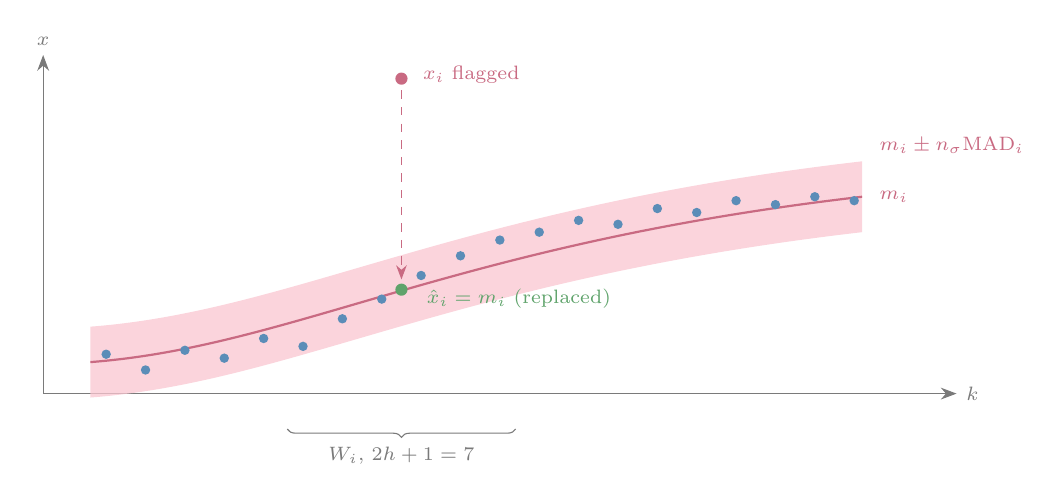
\begin{tikzpicture}[x=1cm,y=1cm]
\draw[-{Stealth[length=2mm]}, dgray] (0,0) -- (11.6,0) node[right, tag] {$k$};
\draw[-{Stealth[length=2mm]}, dgray] (0,0) -- (0,4.3) node[above, tag] {$x$};
% band
\fill[ppink, opacity=0.75]
  (0.6,0.85) .. controls (3.2,1.05) and (5.2,2.35) .. (10.4,2.95) --
  (10.4,2.05) .. controls (5.2,1.45) and (3.2,0.15) .. (0.6,-0.05) -- cycle;
% median curve
\draw[dpink, thick]
  (0.6,0.4) .. controls (3.2,0.6) and (5.2,1.9) .. (10.4,2.5);
\node[tag, text=dpink, anchor=west] at (10.5,2.5) {$m_i$};
\node[tag, text=dpink, anchor=west] at (10.5,3.15) {$m_i \pm n_\sigma \mathrm{MAD}_i$};
% points
\foreach \x/\y in {0.8/0.5,1.3/0.3,1.8/0.55,2.3/0.45,2.8/0.7,3.3/0.6,3.8/0.95,
                   4.3/1.2,4.8/1.5,5.3/1.75,5.8/1.95,6.3/2.05,6.8/2.2,7.3/2.15,
                   7.8/2.35,8.3/2.3,8.8/2.45,9.3/2.4,9.8/2.5,10.3/2.45}
  {\fill[dblue] (\x,\y) circle (1.7pt);}
% flagged
\fill[dpink] (4.55,4.0) circle (2.2pt);
\node[tag, text=dpink, anchor=west] at (4.7,4.05) {$x_i$ flagged};
\draw[dashed, dpink, -{Stealth[length=1.8mm]}] (4.55,3.85) -- (4.55,1.45);
\fill[dgreen] (4.55,1.32) circle (2.2pt);
\node[tag, text=dgreen, anchor=west] at (4.75,1.2) {$\hat x_i = m_i$ (replaced)};
% window brace
\draw[decorate, decoration={brace, amplitude=3pt, mirror}, dgray] (3.1,-0.45) -- (6.0,-0.45)
      node[midway, below=3pt, tag] {$W_i$, $2h+1 = 7$};
\end{tikzpicture}
\caption{Hampel screen, Eq.~\eqref{eq:hampel}: the flagged sample is replaced by
the local median.}
\label{fig:hampelfig}
\end{figure}

% ---------------------------------------------------------------------
\subsection{Stage 2: constant-jerk Kalman filter with RTS smoother}
% ---------------------------------------------------------------------

\paragraph{Continuous-time model.} Per axis, let
$\bm{s}(t) = [p, v, a]^{\!\top}$ (position, velocity, acceleration) and model
jerk as white noise $w(t)$ with power spectral density $q$:
\begin{equation}
  \dot{\bm{s}} = \bm{A}\bm{s} + \bm{G}w,
  \qquad
  \bm{A} = \begin{bmatrix} 0&1&0\\ 0&0&1\\ 0&0&0 \end{bmatrix},
  \qquad
  \bm{G} = \begin{bmatrix} 0\\0\\1 \end{bmatrix},
  \qquad
  \mathbb{E}[w(t)w(t')] = q\,\delta(t-t').
  \label{eq:ctmodel}
\end{equation}

\paragraph{Exact discretization over a step $\Delta t$.} Because $\bm{A}$ is
nilpotent ($\bm{A}^3 = 0$), the transition matrix is a finite sum,
\begin{equation}
  \bm{F}(\Delta t) = e^{\bm{A}\Delta t}
  = \bm{I} + \bm{A}\Delta t + \tfrac12 \bm{A}^2 \Delta t^2
  = \begin{bmatrix}
      1 & \Delta t & \Delta t^2/2\\
      0 & 1        & \Delta t\\
      0 & 0        & 1
    \end{bmatrix},
  \label{eq:F}
\end{equation}
and the process-noise covariance is the integral
\begin{equation}
  \bm{Q}(\Delta t) = \int_0^{\Delta t} \bm{F}(\varsigma)\,\bm{G}\,q\,\bm{G}^{\!\top}\bm{F}(\varsigma)^{\!\top} d\varsigma
  = q \begin{bmatrix}
      \Delta t^5/20 & \Delta t^4/8 & \Delta t^3/6\\
      \Delta t^4/8  & \Delta t^3/3 & \Delta t^2/2\\
      \Delta t^3/6  & \Delta t^2/2 & \Delta t
    \end{bmatrix},
  \label{eq:Q}
\end{equation}
since $\bm{F}(\varsigma)\bm{G} = [\varsigma^2/2,\ \varsigma,\ 1]^{\!\top}$ and
entry $(i,j)$ integrates the product of the corresponding components. Both
matrices are recomputed at every step with the trial's own
$\Delta t_k = t_k - t_{k-1}$; this is what makes the filter exact on irregular
timestamps, and it is the property that a fixed-frequency filter cannot offer.

\paragraph{Measurement.} Only position is observed:
\begin{equation}
  z_k = \bm{H}\bm{s}_k + \nu_k,
  \qquad \bm{H} = [1\ 0\ 0],
  \qquad \nu_k \sim \mathcal{N}(0, R),
  \qquad R = \sigma_{\text{meas}}^2 = 2^2\ \text{px}^2 .
  \label{eq:meas}
\end{equation}

\paragraph{Initialization.} With $\Delta t_0 = t_1 - t_0$ and
$\sigma_{a,0} = 20\,\sigma_{\text{jerk}}\operatorname{median}_k(\Delta t_k)$,
\begin{equation}
  \hat{\bm{s}}_0^- = \big[\, z_0,\ (z_1 - z_0)/\Delta t_0,\ 0 \,\big]^{\!\top},
  \qquad
  \bm{P}_0^- = \operatorname{diag}\!\big(R,\ 2R/\Delta t_0^2,\ \sigma_{a,0}^2\big).
  \label{eq:init}
\end{equation}
The velocity variance $2R/\Delta t_0^2$ is the variance of a finite difference
of two independent measurements; the factor 20 in $\sigma_{a,0}$ is a heuristic
inflation so the acceleration prior is uninformative.

\paragraph{Forward recursion (predict / update), $k = 1, \dots, n-1$.}
\begin{align}
  \hat{\bm{s}}_k^- &= \bm{F}_k \hat{\bm{s}}_{k-1},
  &\bm{P}_k^- &= \bm{F}_k \bm{P}_{k-1} \bm{F}_k^{\!\top} + \bm{Q}_k, \label{eq:kf1}\\
  y_k &= z_k - \hat p_k^-,
  &S_k &= [\bm{P}_k^-]_{11} + R, \label{eq:kf2}\\
  \bm{K}_k &= \bm{P}_k^- \bm{H}^{\!\top} / S_k = [\bm{P}_k^-]_{:,1}/S_k, & & \label{eq:kf3}\\
  \hat{\bm{s}}_k &= \hat{\bm{s}}_k^- + \bm{K}_k y_k,
  &\bm{P}_k &= \bm{P}_k^- - \bm{K}_k [\bm{P}_k^-]_{1,:}, \label{eq:kf4}
\end{align}
followed by symmetrization $\bm{P}_k \leftarrow (\bm{P}_k + \bm{P}_k^{\!\top})/2$
for numerical hygiene. The update is skipped (the prediction is carried forward
and the counter \code{n\_gated} incremented) when the innovation fails the
$\chi^2$ gate $y_k^2 > \gamma^2 S_k$; with the default $\gamma = \infty$ the gate
never fires.

\paragraph{Backward recursion (Rauch--Tung--Striebel).} Starting from
$\hat{\bm{s}}_{n-1}^{s} = \hat{\bm{s}}_{n-1}$, for $k = n-2, \dots, 0$:
\begin{equation}
  \bm{C}_k = \bm{P}_k \bm{F}_{k+1}^{\!\top} \big(\bm{P}_{k+1}^-\big)^{-1},
  \qquad
  \hat{\bm{s}}_k^{s} = \hat{\bm{s}}_k + \bm{C}_k\big(\hat{\bm{s}}_{k+1}^{s} - \hat{\bm{s}}_{k+1}^{-}\big).
  \label{eq:rts}
\end{equation}
Only the state is smoothed (the smoothed covariance is not needed downstream).
The stage output is the smoothed position $\hat p_k^{s}$; the smoothed velocity
and acceleration are discarded, because the kinematics are recomputed after
resampling and low-pass filtering. Figure~\ref{fig:kalmanbox} shows the arrays
the implementation keeps so that Eq.~\eqref{eq:rts} can run backward, and
Figure~\ref{fig:rtslag} shows why the backward pass matters.

\begin{figure}[htbp]
\centering
\resizebox{0.98\textwidth}{!}{%
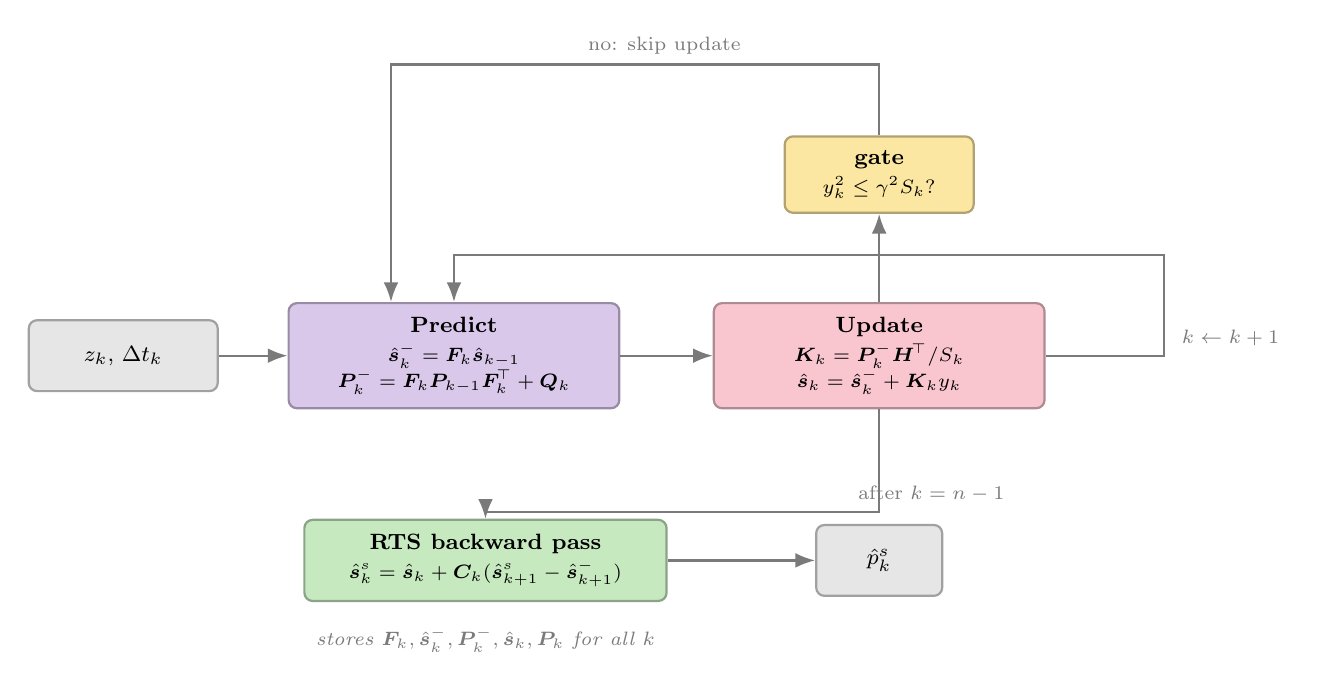
\begin{tikzpicture}
\node[blk=pgray,   minimum width=24mm] (in)  at (0.0,0) {$z_k$, $\Delta t_k$};
\node[blk=ppurple, minimum width=42mm] (pre) at (4.2,0)
  {\textbf{Predict}\\[1pt]\scriptsize $\hat{\bm{s}}_k^- = \bm{F}_k\hat{\bm{s}}_{k-1}$\\
   \scriptsize $\bm{P}_k^- = \bm{F}_k\bm{P}_{k-1}\bm{F}_k^{\!\top} + \bm{Q}_k$};
\node[blk=ppink,   minimum width=42mm] (upd) at (9.6,0)
  {\textbf{Update}\\[1pt]\scriptsize $\bm{K}_k = \bm{P}_k^-\bm{H}^{\!\top}/S_k$\\
   \scriptsize $\hat{\bm{s}}_k = \hat{\bm{s}}_k^- + \bm{K}_k y_k$};
\node[blk=pyellow, minimum width=24mm] (gate) at (9.6,2.3) {\textbf{gate}\\[1pt]\scriptsize $y_k^2 \le \gamma^2 S_k$?};
\node[blk=pgreen,  minimum width=46mm] (rts) at (4.6,-2.6)
  {\textbf{RTS backward pass}\\[1pt]\scriptsize $\hat{\bm{s}}_k^{s} = \hat{\bm{s}}_k + \bm{C}_k(\hat{\bm{s}}_{k+1}^{s} - \hat{\bm{s}}_{k+1}^{-})$};
\node[blk=pgray,   minimum width=16mm] (out) at (9.6,-2.6) {$\hat p_k^{s}$};
\draw[lane] (in) -- (pre);
\draw[lane] (pre) -- (upd);
\draw[lane] (upd) -- (gate);
\draw[lane] (gate.north) -- ++(0,0.9) -| node[tag, above, pos=0.22] {no: skip update} ([xshift=-8mm]pre.north);
\draw[lane] (upd.east) -- ++(1.5,0) node[tag, above right=0pt and 1mm] {$k \leftarrow k+1$}
      |- ([yshift=6mm]pre.north) -- (pre.north);
\draw[lane] (upd.south) -- ++(0,-1.3) -| node[tag, above right=0pt and 1mm, pos=0.05] {after $k = n-1$} (rts.north);
\draw[lane] (rts) -- (out);
\node[note, below=2mm of rts] {stores $\bm{F}_k, \hat{\bm{s}}_k^-, \bm{P}_k^-, \hat{\bm{s}}_k, \bm{P}_k$ for all $k$};
\end{tikzpicture}}
\caption{Structure of \code{KalmanTrajectorySmoother.\_\_call\_\_}. The arrays
\code{xp}, \code{pp}, \code{xf}, \code{pf}, \code{fk} hold the predicted and
filtered quantities so Eq.~\eqref{eq:rts} can run backward.}
\label{fig:kalmanbox}
\end{figure}

\paragraph{What the parameters actually do.} The filter has one free ratio,
$q/R$. A useful order-of-magnitude rule for a $\nu$-th order
integrated-white-noise model observed in position is that the steady-state
estimator behaves like a low-pass with corner
$\omega_0 \sim (q/R)^{1/(2\nu)}$; here $\nu = 3$, so
\begin{equation}
  \omega_0 \sim \left(\frac{q}{R}\right)^{1/6}
  = \left(\frac{(10^5)^2}{2^2}\right)^{1/6} \approx 37\ \text{rad/s} \approx 5.9\ \text{Hz}.
  \label{eq:corner}
\end{equation}
With the defaults ($\sigma_{\text{jerk}} = 10^5$ px/s$^3$,
$\sigma_{\text{meas}} = 2$ px) the Kalman stage therefore smooths at roughly the
same scale as the 6~Hz Butterworth that follows, which is consistent. Raising
$\sigma_{\text{jerk}}$ makes the stage closer to a pass-through; lowering it
increases smoothing and, because the RTS pass is non-causal, does so without
lag. This scaling is a heuristic, not an exact bandwidth; it is offered to give
the two parameters an interpretable scale.

\begin{figure}[htbp]
\centering
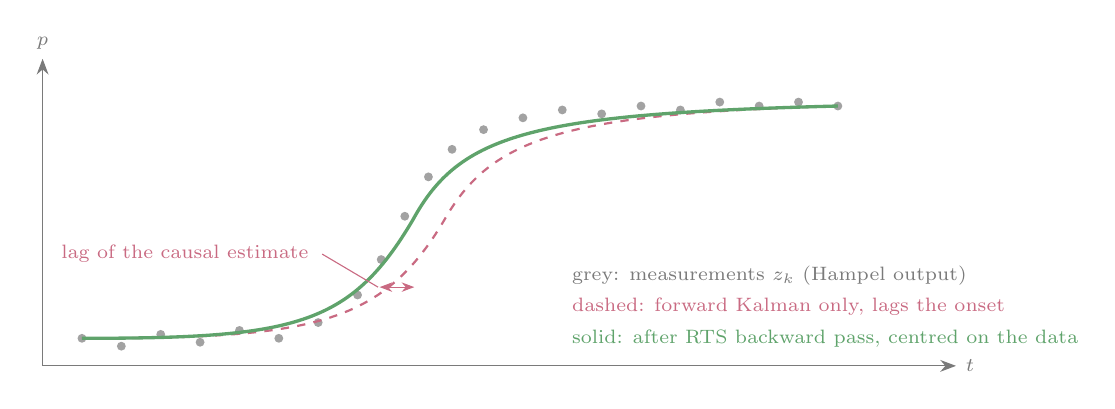
\begin{tikzpicture}[x=1cm,y=1cm]
\draw[-{Stealth[length=2mm]}, dgray] (0,0) -- (11.6,0) node[right, tag] {$t$};
\draw[-{Stealth[length=2mm]}, dgray] (0,0) -- (0,3.9) node[above, tag] {$p$};
% measurements
\foreach \x/\y in {0.5/0.35,1.0/0.25,1.5/0.4,2.0/0.3,2.5/0.45,3.0/0.35,3.5/0.55,
                   4.0/0.9,4.3/1.35,4.6/1.9,4.9/2.4,5.2/2.75,5.6/3.0,6.1/3.15,
                   6.6/3.25,7.1/3.2,7.6/3.3,8.1/3.25,8.6/3.35,9.1/3.3,9.6/3.35,10.1/3.3}
  {\fill[dgray!70] (\x,\y) circle (1.6pt);}
% causal (lagging) estimate
\draw[dpink, thick, dashed]
  (0.5,0.35) .. controls (3.4,0.35) and (4.3,0.5) .. (5.1,1.85)
             .. controls (5.7,2.9) and (6.6,3.2) .. (10.1,3.3);
% smoothed
\draw[dgreen, very thick]
  (0.5,0.35) .. controls (3.2,0.35) and (3.9,0.5) .. (4.7,1.85)
             .. controls (5.3,2.95) and (6.2,3.2) .. (10.1,3.3);
% lag marker
\draw[{Stealth[length=1.6mm]}-{Stealth[length=1.6mm]}, dpink] (4.28,1.00) -- (4.72,1.00);
\draw[dpink] (4.26,1.00) -- (3.55,1.42);
\node[tag, text=dpink, anchor=east] at (3.50,1.42) {lag of the causal estimate};
\node[tag, anchor=west, text=dgray]  at (6.6,1.15) {grey: measurements $z_k$ (Hampel output)};
\node[tag, anchor=west, text=dpink]  at (6.6,0.75) {dashed: forward Kalman only, lags the onset};
\node[tag, anchor=west, text=dgreen] at (6.6,0.35) {solid: after RTS backward pass, centred on the data};
\end{tikzpicture}
\caption{Why the backward pass matters: a causal filter can only react after the
change has happened, so its estimate of a movement onset is late by roughly its
time constant. The RTS pass revisits every estimate with the whole trial in hand
and removes that delay, which is what makes onset and peak times usable
offline.}
\label{fig:rtslag}
\end{figure}

% ---------------------------------------------------------------------
\subsection{Stage 3: PCHIP resampling to a uniform grid}
% ---------------------------------------------------------------------

\paragraph{Grid.} \code{\_build\_grid} produces
$t_g^{(m)} = t_0 + m\Delta$, $m = 0, 1, \dots$, up to $t_{n-1}$, with
$\Delta = \code{grid\_dt\_s} = 0.008$~s. The tail is handled so the last grid
point equals $t_{n-1}$: if the leftover $t_{n-1} - t_g^{(M)}$ exceeds $\Delta/4$
the endpoint is appended, otherwise the last grid point is moved onto it. The
final interval is therefore not exactly $\Delta$; the kinematics use the actual
\code{diff} of the grid, so this introduces no error. If the whole trial is
shorter than $\Delta$ the grid is just $[t_0, t_{n-1}]$.

\paragraph{Interpolant.} On each interval $[t_i, t_{i+1}]$ PCHIP builds the
cubic Hermite polynomial
\begin{equation}
  P(t) = \hat p_i^{s} h_{00}(u) + \delta_i d_i h_{10}(u)
       + \hat p_{i+1}^{s} h_{01}(u) + \delta_i d_{i+1} h_{11}(u),
  \qquad u = \frac{t - t_i}{\delta_i},\ \ \delta_i = t_{i+1} - t_i,
  \label{eq:pchip}
\end{equation}
with the standard Hermite basis $h_{00}, h_{10}, h_{01}, h_{11}$ and endpoint
slopes $d_i$ chosen by the Fritsch--Carlson rule: if the secants
$\sigma_{i-1} = (\hat p_i^{s} - \hat p_{i-1}^{s})/\delta_{i-1}$ and $\sigma_i$
have opposite signs or one is zero, then $d_i = 0$; otherwise $d_i$ is the
weighted harmonic mean
\begin{equation}
  d_i = \frac{w_1 + w_2}{w_1/\sigma_{i-1} + w_2/\sigma_i},
  \qquad w_1 = 2\delta_i + \delta_{i-1},\ \ w_2 = \delta_i + 2\delta_{i-1}.
  \label{eq:fritsch}
\end{equation}
The result is $C^1$, preserves monotonicity of the data between samples, and
cannot overshoot at a sharp movement onset, unlike a natural cubic spline. The
second derivative is discontinuous at the knots, which is acceptable because
acceleration is never taken from this interpolant.

\begin{figure}[htbp]
\centering
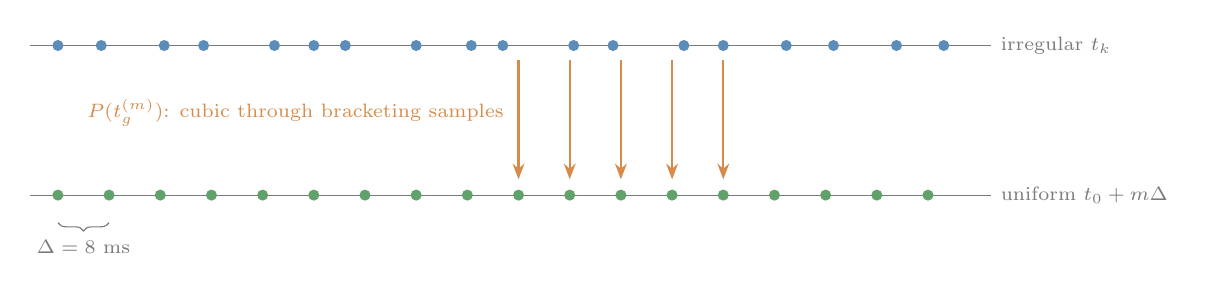
\begin{tikzpicture}[x=1cm,y=1cm]
% irregular
\draw[dgray] (0,1.9) -- (12.2,1.9) node[right, tag] {irregular $t_k$};
\foreach \x in {0.35,0.9,1.7,2.2,3.1,3.6,4.0,4.9,5.6,6.0,6.9,7.4,8.3,8.8,9.6,10.2,11.0,11.6}
  {\fill[dblue] (\x,1.9) circle (2pt);}
% uniform
\draw[dgray] (0,0) -- (12.2,0) node[right, tag] {uniform $t_0 + m\Delta$};
\foreach \x in {0.35,1.0,1.65,2.3,2.95,3.6,4.25,4.9,5.55,6.2,6.85,7.5,8.15,8.8,9.45,10.1,10.75,11.4}
  {\fill[dgreen] (\x,0) circle (2pt);}
\draw[decorate, decoration={brace, amplitude=3pt, mirror}, dgray] (0.35,-0.35) -- (1.0,-0.35)
      node[midway, below=3pt, tag] {$\Delta = 8$ ms};
% arrows
\foreach \x in {6.2,6.85,7.5,8.15,8.8}
  {\draw[-{Stealth[length=2mm]}, dorange, thick] (\x,1.72) -- (\x,0.2);}
\node[tag, text=dorange, anchor=west, align=left] at (0.6,1.05)
  {$P(t_g^{(m)})$: cubic through bracketing samples};
\end{tikzpicture}
\caption{Resampling from the raw irregular clock onto the 125 Hz grid.}
\label{fig:pchip}
\end{figure}

\begin{figure}[htbp]
\centering
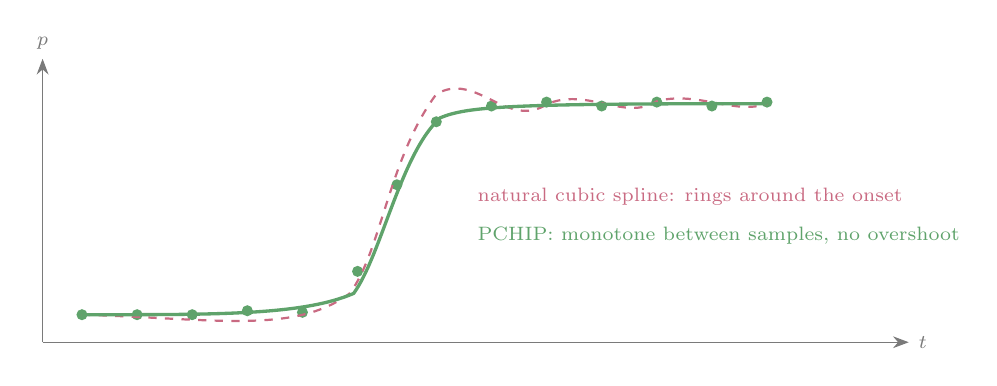
\begin{tikzpicture}[x=1cm,y=1cm]
\draw[-{Stealth[length=2mm]}, dgray] (0,0) -- (11.0,0) node[right, tag] {$t$};
\draw[-{Stealth[length=2mm]}, dgray] (0,0) -- (0,3.6) node[above, tag] {$p$};
\foreach \x/\y in {0.5/0.35,1.2/0.35,1.9/0.35,2.6/0.4,3.3/0.38,4.0/0.9,4.5/2.0,
                   5.0/2.8,5.7/3.0,6.4/3.05,7.1/3.0,7.8/3.05,8.5/3.0,9.2/3.05}
  {\fill[dgreen] (\x,\y) circle (2pt);}
% spline (ringing)
\draw[dpink, dashed, thick]
  (0.5,0.35) .. controls (2.2,0.3) and (3.2,0.1) .. (3.9,0.62)
             .. controls (4.3,1.15) and (4.4,2.35) .. (5.0,3.15)
             .. controls (5.5,3.45) and (5.9,2.7) .. (6.4,3.02)
             .. controls (6.9,3.25) and (7.4,2.8) .. (7.8,3.06)
             .. controls (8.3,3.2) and (8.8,2.88) .. (9.2,3.03);
% pchip
\draw[dgreen, very thick]
  (0.5,0.35) .. controls (2.2,0.35) and (3.3,0.34) .. (3.95,0.62)
             .. controls (4.3,1.1) and (4.55,2.4) .. (5.05,2.85)
             .. controls (5.4,3.0) and (6.0,3.03) .. (9.2,3.03);
\node[tag, text=dpink,  anchor=west] at (5.4,1.85) {natural cubic spline: rings around the onset};
\node[tag, text=dgreen, anchor=west] at (5.4,1.35) {PCHIP: monotone between samples, no overshoot};
\end{tikzpicture}
\caption{Why PCHIP rather than a smoothing spline: at a reaching onset the data
go from still to moving within one or two samples, and a spline invents
oscillations there that a differentiator would later read as acceleration.}
\label{fig:pchipspline}
\end{figure}

\paragraph{Rate reduction.} Raw \code{rz2adc} data arrive at $\approx 939$~Hz,
so the 125~Hz grid is a $\sim 7.5\times$ decimation. No anti-alias filter is
applied between stages 2 and 3: the Kalman stage acts as one (see
Eq.~\eqref{eq:corner}) and any residual content between 6~Hz and 62.5~Hz is
removed by stage 4. Content above the new Nyquist frequency (62.5~Hz) would
alias, but joystick signals that survive stage 2 have no meaningful power there.
If a much larger $\sigma_{\text{jerk}}$ were chosen (weaker Kalman smoothing),
this assumption should be re-checked.

% ---------------------------------------------------------------------
\subsection{Stage 4: zero-phase Butterworth low-pass}
% ---------------------------------------------------------------------

\paragraph{Analog prototype.} A second-order Butterworth low-pass with cutoff
$\omega_c$ has
\begin{equation}
  |H_a(j\omega)|^2 = \frac{1}{1 + (\omega/\omega_c)^{4}},
  \qquad
  H_a(s) = \frac{1}{\bar s^2 + \sqrt2\,\bar s + 1},
  \quad \bar s = s/\omega_c .
  \label{eq:butter}
\end{equation}

\paragraph{Bilinear transform with prewarping.} Substituting
$\bar s = \frac{1}{K}\frac{1 - z^{-1}}{1 + z^{-1}}$ with
$K = \tan(\pi f_c/f_s)$ maps the analog cutoff exactly onto the digital $f_c$
and gives
\begin{equation}
  H(z) = \frac{K^2\,(1 + 2z^{-1} + z^{-2})}
              {(1 + \sqrt2 K + K^2) + 2(K^2 - 1)z^{-1} + (1 - \sqrt2 K + K^2)z^{-2}} .
  \label{eq:butterz}
\end{equation}
Normalizing by $a_0 = 1 + \sqrt2 K + K^2$ yields exactly the arrays in
\code{ButterworthLowpass.\_design}:

\begin{lstlisting}[language=Python]
k    = np.tan(np.pi * self.cutoff_hz / fs)
norm = 1.0 / (1.0 + np.sqrt(2.0) * k + k ** 2)
b    = np.array([k ** 2, 2.0 * k ** 2, k ** 2]) * norm
a    = np.array([1.0, 2.0 * (k ** 2 - 1.0) * norm,
                 (1.0 - np.sqrt(2.0) * k + k ** 2) * norm])
\end{lstlisting}

\noindent
With $f_c = 6$~Hz and $f_s = 125$~Hz, $K = \tan(0.1508) \approx 0.1519$.

\paragraph{Forward--backward application.} The filter is run forward, the output
is reversed, run again, and reversed back. The effective response is
\begin{equation}
  H_{\text{eff}}(e^{j\omega}) = H(e^{j\omega})\,H(e^{-j\omega}) = |H(e^{j\omega})|^2,
  \qquad \angle H_{\text{eff}} = 0,
  \label{eq:filtfilt}
\end{equation}
so the magnitude is squared (stop-band attenuation doubles in dB) and the phase
is identically zero. The price is a shift of the $-3$~dB point: solving
$|H|^4 = 1/2$ gives $(\omega/\omega_c)^4 = \sqrt2 - 1$, i.e.
\begin{equation}
  f_{-3\text{dB}}^{\text{eff}} = (\sqrt2 - 1)^{1/4} f_c \approx 0.802\,f_c \approx 4.8\ \text{Hz}.
  \label{eq:effcut}
\end{equation}
For $p$ passes of an order-$N$ Butterworth the general ratio is
$\big(2^{1/p} - 1\big)^{1/(2N)}$. The notebook computes the digital value on the
prewarped axis rather than quoting the analog one, so the figure titles stay
correct if either parameter changes:

\begin{lstlisting}[language=Python]
def effective_cutoff_hz(cutoff_hz=CUTOFF_HZ, fs_hz=1.0 / GRID_DT_S, order=2, n_passes=2):
    ratio = (2.0 ** (1.0 / n_passes) - 1.0) ** (1.0 / (2.0 * order))
    return float(fs_hz / np.pi * np.arctan(ratio * np.tan(np.pi * cutoff_hz / fs_hz)))
EFFECTIVE_CUTOFF_HZ = effective_cutoff_hz()          # 4.82 Hz at fc = 6, fs = 125
\end{lstlisting}

\noindent
This is the number to keep in mind when reading ``6~Hz'': the two-pass filter is
half-power at about 4.8~Hz and reaches $-6$~dB at 6~Hz.

\begin{figure}[htbp]
\centering
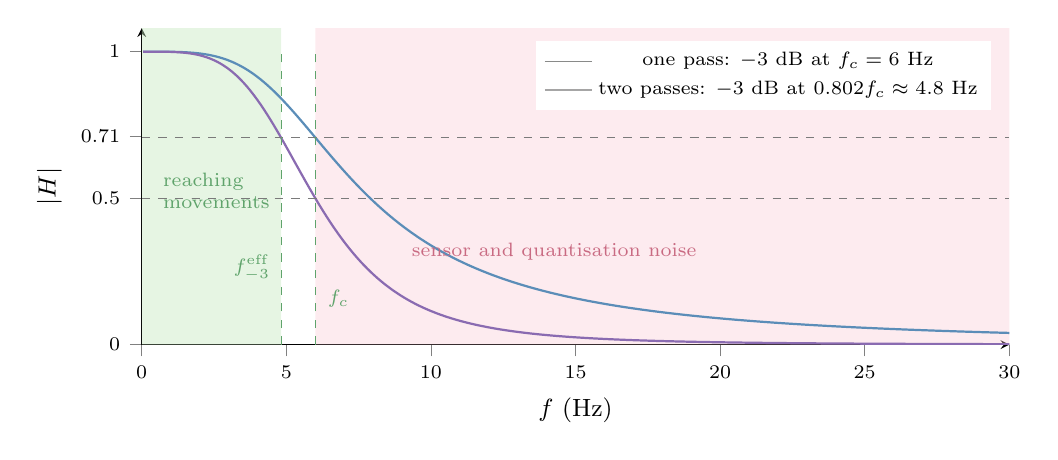
\begin{tikzpicture}
\begin{axis}[
  width=12.6cm, height=5.6cm,
  xlabel={$f$ (Hz)}, ylabel={$|H|$},
  domain=0.05:30, samples=260,
  xmin=0, xmax=30, ymin=0, ymax=1.08,
  axis lines=left, tick align=outside,
  ytick={0,0.5,0.71,1}, yticklabels={0,0.5,0.71,1},
  legend style={draw=none, font=\scriptsize, at={(0.98,0.96)}, anchor=north east},
  tick label style={font=\scriptsize},
  every axis x label/.style={at={(ticklabel cs:0.5)}, anchor=near ticklabel, font=\small},
  every axis y label/.style={at={(ticklabel cs:0.5)}, rotate=90, anchor=near ticklabel, font=\small},
]
\addplot[fill=pgreen, draw=none, opacity=0.45, domain=0:4.82] {1.08} \closedcycle;
\addplot[fill=ppink,  draw=none, opacity=0.35, domain=6:30]   {1.08} \closedcycle;
\addplot[dblue, thick]   {1/sqrt(1 + (x/6)^4)};
\addlegendentry{one pass: $-3$ dB at $f_c = 6$ Hz}
\addplot[dpurple, thick] {1/(1 + (x/6)^4)};
\addlegendentry{two passes: $-3$ dB at $0.802 f_c \approx 4.8$ Hz}
\addplot[dgray, dashed, domain=0:30] {0.7071};
\addplot[dgray, dashed, domain=0:30] {0.5};
\draw[dgreen, dashed] (axis cs:4.82,0) -- (axis cs:4.82,1.0);
\draw[dgreen, dashed] (axis cs:6,0) -- (axis cs:6,1.0);
\node[tag, text=dgreen, anchor=north east] at (axis cs:4.78,0.34) {$f^{\text{eff}}_{-3}$};
\node[tag, text=dgreen, anchor=north west] at (axis cs:6.1,0.22) {$f_c$};
\node[tag, text=dgreen, anchor=north west, font=\scriptsize, align=left] at (axis cs:0.4,0.62)
      {reaching\\movements};
\node[tag, text=dpink,  anchor=north west, font=\scriptsize] at (axis cs:9.0,0.38)
      {sensor and quantisation noise};
\end{axis}
\end{tikzpicture}
\caption{Magnitude response of the analog prototype (one pass) and of the
forward--backward application (two passes). The bilinear transform preserves
these curves up to frequency warping, which the prewarped $K$ pins exactly at
$f_c$.}
\label{fig:butter}
\end{figure}

\paragraph{Edge handling.} Two devices suppress start-up transients, both
mirroring \code{scipy.signal.filtfilt} defaults:
\begin{enumerate}[leftmargin=*,itemsep=1pt]
\item \emph{Odd reflection padding} of $n_f = 6$ samples at each end,
$\tilde x_{-j} = 2x_0 - x_j$ and $\tilde x_{n-1+j} = 2x_{n-1} - x_{n-1-j}$,
$j = 1..n_f$; the padded region is discarded after filtering
(\code{ext[nf:-nf]}). Here $n_f = 3\cdot\max(\operatorname{len}(a),
\operatorname{len}(b)) - 3 = 6$.
\item \emph{Steady-state initial conditions.} For the transposed direct-form II
realization with state $\bm{\zeta}$, the state that reproduces a constant input
$x$ as a constant output satisfies $(\bm{I} - \bm{A}_c)\bm{\zeta} = \bm{b}'$ with
companion matrix
$\bm{A}_c = \begin{bmatrix} -a_1 & 1\\ -a_2 & 0\end{bmatrix}$ and
$\bm{b}' = [b_1 - a_1 b_0,\ b_2 - a_2 b_0]^{\!\top}$.
\code{\_steady\_state} solves this once and scales the result by the first
padded sample (\code{zi * ext[0]}).
\end{enumerate}
The filter is skipped (\code{applied = False}) when $n \le n_f$ or when
$f_c \ge f_s/2$, and the per-trial figure title says which of the two happened.

\paragraph{Why here and why zero-phase.} Voluntary reaching movements carry
essentially no power above a few Hz; what remains above $\sim 6$~Hz on the
125~Hz grid is quantisation and sensor noise. A causal filter would delay every
kinematic event by its group delay (tens of ms at these settings), which would
bias movement-onset and peak-speed times; zero phase removes the noise without
moving any feature.

% ---------------------------------------------------------------------
\subsection{Stage 5: speed, Savitzky--Golay acceleration, summary window}
\label{sec:summary}
% ---------------------------------------------------------------------

\paragraph{Speed.} On the grid, with actual steps
$g_k = t_g^{(k+1)} - t_g^{(k)}$ (all $= \Delta$ except possibly the last),
\begin{equation}
  v_k = \frac{\sqrt{(x_{k+1}-x_k)^2 + (y_{k+1}-y_k)^2}}{g_k},
  \qquad
  t_k^{(v)} = t_g^{(k)} + \frac{g_k}{2},
  \qquad
  v_k^{\text{cm}} = c\,v_k .
  \label{eq:speed}
\end{equation}
This is a central-difference estimate located at the segment midpoint
(\code{np.hypot(np.diff(...))} divided by \code{np.diff(t)}). Because
$v_k \ge 0$ by construction it is speed, not signed velocity.

\paragraph{Tangential acceleration via Savitzky--Golay.} Rather than
differencing $v_k$ again, in a sliding window of $w = 11$ samples
($\approx 88$~ms at 125~Hz) a polynomial of degree $p = 3$ is fitted by least
squares and differentiated analytically at the window centre:
\begin{equation}
  \hat v(u) = \sum_{j=0}^{p}\beta_j u^j,
  \qquad
  \bm{\beta} = (\bm{V}^{\!\top}\bm{V})^{-1}\bm{V}^{\!\top}\bm{v}_{k-h:k+h},
  \qquad
  a_k = \frac{|\beta_1|}{\Delta},
  \label{eq:savgol}
\end{equation}
where $\bm{V}$ is the $w \times (p+1)$ Vandermonde matrix on
$u = -h, \dots, h$, $h = (w-1)/2$. Because $\bm{V}$ is fixed,
$(\bm{V}^{\!\top}\bm{V})^{-1}\bm{V}^{\!\top}$ is a fixed $(p+1)\times w$ matrix
and $a_k$ is a convolution of $\bm{v}$ with its second row (the derivative
filter). The absolute value is taken, so $a_k$ is the magnitude of the
tangential acceleration $|d|\bm{v}|/dt|$, in cm/s$^2$. The step passed to
\code{savgol\_filter} is $\operatorname{median}(g_k)$, not $\Delta$, so a grid
whose last interval was shortened is handled correctly.

\paragraph{Why not a second finite difference.} Differentiation multiplies the
noise spectrum by $\omega^2$ (in power); a bare difference of $v_k$ would let
single-sample jitter dominate $\max_k a_k$. The least-squares fit acts as a
low-pass before the derivative is taken, and the 99th percentile
(\code{ACCEL\_PEAK\_PERCENTILE}) is used as the ``peak'' so that one residual
spike does not set the value.

\paragraph{Window fallbacks (\code{\_savgol\_accel}).}
$w \leftarrow \min(w, n$ or $n-1)$ forced odd and $\ge 5$;
$p \leftarrow \min(p, w-1)$. For $n < 5$ the code uses \code{np.gradient}
instead; $n = 1$ returns 0 and $n = 0$ returns an empty array.

\paragraph{Summary window: takeoff to target entry.} Every per-trial summary is
taken over the same samples. Let $\mathcal{S}$ be the speed samples whose
midpoint time falls at or before the last \code{MOVEMENT} sample (target entry),
taken from the \code{Epoch} column; if the trial has no \code{MOVEMENT} epoch
(an early exit) the search falls back to all samples.

\emph{Which peak the walk-back starts from.} Inside $\mathcal{S}$ the local
maxima of $v$ are found with \code{scipy.signal.find\_peaks} under a prominence
threshold of $\code{MULTI\_PEAK\_PROMINENCE\_FRAC} = 0.15$ times the largest
speed in $\mathcal{S}$, and their count is recorded as \code{n\_speed\_peaks}
(at least 1). With $\code{TAKEOFF\_PEAK\_CHOICE} = \code{"first"}$, the default,
$k^\star$ is the \emph{first} of those peaks; with any other value it is the
global $\arg\max_{k \in \mathcal{S}} v_k$, which is what the code did before.
The distinction only matters on a trial whose speed profile has more than one
submovement: walking back from the global maximum, which may belong to the
second submovement, would place the takeoff after the first one had already
started, and the movement onset would be late by the whole duration of the
first. The first prominent peak is the one that belongs to the initial reach,
and dating the onset is what the takeoff exists for.

\emph{The walk-back.} With $k^\star$ fixed,
\begin{equation}
  \theta = \rho\, v_{k^\star},
  \qquad
  k_{\text{takeoff}} = \min\{\,k \le k^\star : v_j \ge \theta\ \forall j \in [k, k^\star]\,\},
  \label{eq:takeoff}
\end{equation}
that is, walk backward from $k^\star$ while the speed stays above a fraction
$\rho$ of it; \code{move\_takeoff\_ms} is $t^{(v)}_{k_{\text{takeoff}}}$. The
fraction is not a bare constant: \code{TAKEOFF\_SPEED\_FRAC\_OPTIONS} offers
\code{"5\%"} $= 0.05$ and \code{"10\%"} $= 0.10$, and
\code{TAKEOFF\_SPEED\_FRAC\_CHOICE} (default \code{"5\%"}) selects the one that
\code{MOVE\_SPEED\_FRAC} takes. Both are set with
\code{globals().get(...)}, so a cell run earlier in the notebook can override
either without editing the pipeline.

\emph{The window.} The summary window is
$\mathcal{M} = \{k \in \mathcal{S} : k \ge k_{\text{takeoff}}\}$, and
\emph{every} statistic uses it:
\begin{equation}
  \begin{aligned}
    v_{\text{peak}} &= \max_{k \in \mathcal{M}} v_k, &
    v_{\text{mean}} &= \operatorname{mean}_{k \in \mathcal{M}} v_k, &
    v_{\text{med}} &= \operatorname{median}_{k \in \mathcal{M}} v_k,\\
    a_{\text{peak}} &= \mathrm{P}_{99}\big(\{a_k\}_{k \in \mathcal{M}}\big), &
    a_{\text{mean}} &= \operatorname{mean}_{k \in \mathcal{M}} a_k, &
    a_{\text{med}} &= \operatorname{median}_{k \in \mathcal{M}} a_k .
  \end{aligned}
  \label{eq:summ}
\end{equation}
Note that $v_{\text{peak}}$ is the maximum over $\mathcal{M}$, not $v_{k^\star}$:
on a two-submovement trial the reported peak can belong to the second
submovement while the takeoff was walked back from the first, and
\code{peak\_vel\_time\_ms} records where that maximum actually is.

Restricting the search to target entry is what stops a jitter during the target
hold from being taken as the reach peak, and using one mask for all six
statistics is what makes them comparable with each other. It is also what makes
the same trial give the same summaries in the section 1.1 cell (which loads
epochs $6,7,8$), in the trajectory-EDA variant, and in the feature table (which
load $6,7$): the window no longer depends on which rows happen to be loaded.
\code{window\_start\_ms} and \code{window\_end\_ms} record the window actually
used, and their difference is exported as \code{takeoff\_to\_target\_ms} and,
in seconds, as \code{TakeoffToTargetTime\_s}.

\paragraph{Takeoff lead.} \code{takeoff\_lead\_ms} $=$ \code{move\_onset\_ms}
$-$ \code{move\_takeoff\_ms} is how long the hand was already moving when it
crossed the centre circle, where \code{move\_onset\_ms} is the first
\code{MOVEMENT} timestamp, that is, the row the task used for
\code{t.leaveCenter}. Both times come from rows of the same trajectory, so the
transport latency cancels in the difference. The derived column
\code{TakeoffTime\_s} $=$ \code{DecisionTime\_s} $-$
\code{takeoff\_lead\_ms}$/1000$ places the takeoff on the go signal and the
clock of \code{DecisionTime\_s}.

\begin{figure}[htbp]
\centering
\resizebox{0.98\textwidth}{!}{%
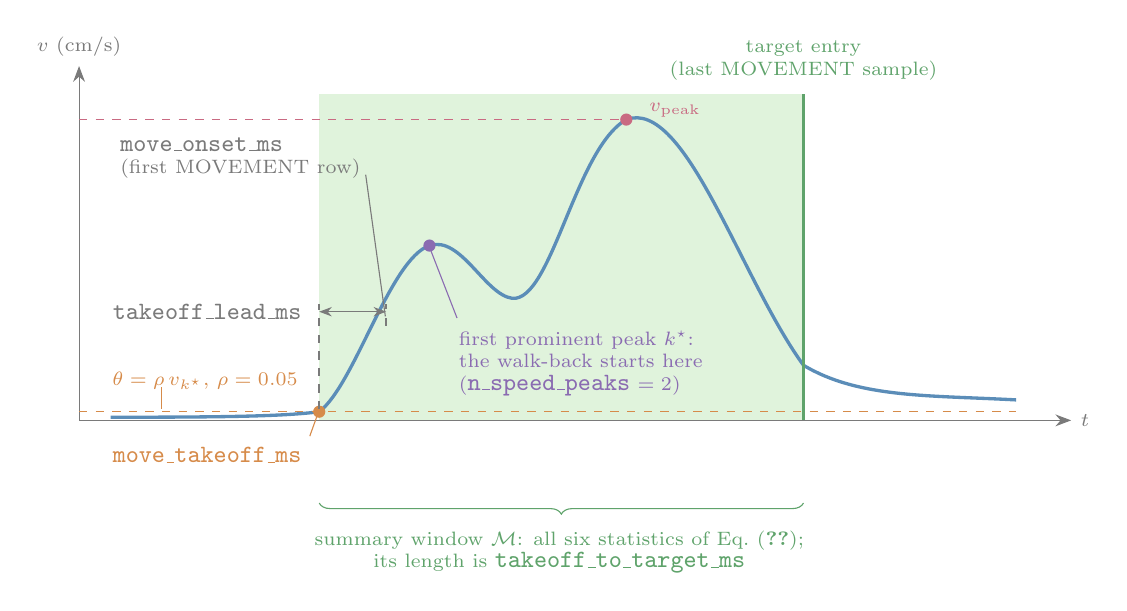
\begin{tikzpicture}[x=1cm,y=1cm]
% --- shading: the summary window ---------------------------------------
\fill[pgreen, opacity=0.55] (3.05,0) rectangle (9.2,4.15);
% --- axes ---------------------------------------------------------------
\draw[-{Stealth[length=2mm]}, dgray] (0,0) -- (12.6,0) node[right, tag] {$t$};
\draw[-{Stealth[length=2mm]}, dgray] (0,0) -- (0,4.5) node[above, tag] {$v$ (cm/s)};
% --- speed profile with two submovements --------------------------------
\draw[dblue, very thick]
  (0.4,0.04)  .. controls (1.8,0.04) and (2.6,0.05) .. (3.05,0.11)
              .. controls (3.50,0.45) and (3.95,2.05) .. (4.45,2.22)
              .. controls (4.85,2.35) and (5.15,1.60) .. (5.50,1.55)
              .. controls (6.00,1.50) and (6.30,3.45) .. (6.95,3.82)
              .. controls (7.70,4.10) and (8.40,1.80) .. (9.20,0.70)
              .. controls (9.90,0.28) and (10.80,0.32) .. (11.90,0.26);
% --- global maximum over M ---------------------------------------------
\draw[dashed, dpink] (0,3.82) -- (6.95,3.82);
\fill[dpink] (6.95,3.82) circle (2.2pt);
\node[tag, text=dpink, anchor=west] at (7.12,3.94) {$v_{\text{peak}}$};
% --- first prominent peak: the walk-back starts here ---------------------
\fill[dpurple] (4.45,2.22) circle (2.2pt);
\draw[dpurple] (4.80,1.30) -- (4.47,2.15);
\node[tag, text=dpurple, anchor=north west, align=left] at (4.70,1.26)
  {first prominent peak $k^\star$:\\the walk-back starts here\\(\code{n\_speed\_peaks} $= 2$)};
% --- takeoff threshold and takeoff --------------------------------------
\draw[dorange, dashed] (0,0.11) -- (11.9,0.11);
\draw[dorange] (1.05,0.42) -- (1.05,0.14);
\node[tag, text=dorange, anchor=west] at (0.30,0.50) {$\theta = \rho\,v_{k^\star}$, $\rho = 0.05$};
\fill[dorange] (3.05,0.11) circle (2.2pt);
\node[tag, text=dorange, anchor=north east, align=right] at (2.95,-0.22) {\code{move\_takeoff\_ms}};
\draw[dorange] (3.02,0.05) -- (2.93,-0.20);
% --- movement onset ------------------------------------------------------
\draw[dgray, thick, dashed] (3.90,1.20) -- (3.90,1.48);
\draw[dgray, thick, dashed] (3.05,0.14) -- (3.05,1.48);
\node[tag, anchor=north west, align=left] at (0.40,3.72)
  {\code{move\_onset\_ms}\\(first MOVEMENT row)};
\draw[dgray] (3.64,3.12) -- (3.89,1.32);
% --- takeoff lead --------------------------------------------------------
\draw[{Stealth[length=1.6mm]}-{Stealth[length=1.6mm]}, dgray] (3.05,1.38) -- (3.90,1.38);
\node[tag, anchor=east] at (2.95,1.38) {\code{takeoff\_lead\_ms}};
% --- target entry --------------------------------------------------------
\draw[dgreen, thick] (9.2,0) -- (9.2,4.15);
\node[tag, text=dgreen, anchor=south, align=center] at (9.2,4.20)
  {target entry\\(last MOVEMENT sample)};
% --- the window ----------------------------------------------------------
\draw[decorate, decoration={brace, amplitude=4pt, mirror}, dgreen] (3.05,-1.05) -- (9.2,-1.05);
\node[tag, text=dgreen, anchor=north, align=center] at (6.1,-1.28)
  {summary window $\mathcal{M}$: all six statistics of Eq.~\eqref{eq:summ};\\
   its length is \code{takeoff\_to\_target\_ms}};
\end{tikzpicture}}
\caption{The summary window on a trial with two submovements. Local peaks are
found inside the search region (up to target entry); the walk-back to
$\theta = 5\,\%$ starts from the \emph{first} prominent one, so the takeoff
dates the initial reach rather than the second submovement. Peak, mean and
median of speed and acceleration are then taken over the whole shaded interval,
which is why $v_{\text{peak}}$ can belong to a later peak than $k^\star$.}
\label{fig:summarywindow}
\end{figure}

% ---------------------------------------------------------------------
\subsection{Data-quality flags}
\label{sec:flags}
% ---------------------------------------------------------------------

Three flags are computed, two of them from raw rows in
\code{TrajectoryDataset.trials} and one in \code{TrialFigure.build}:
\begin{align}
  \code{under\_resolved} \ &\iff\ n < 5, \label{eq:flag1}\\
  \code{hold\_unstable} \ &\iff\ e_{\text{hold}} > r_{\text{target}},
    \qquad e_{\text{hold}} = \max_{k \in \text{hold}} \sqrt{(x_k - x_{h_0})^2 + (y_k - y_{h_0})^2},
    \label{eq:flag2}\\
  \code{hold\_incomplete} \ &\iff\ d_{\text{hold}} < 0.8\cdot\operatorname{median}_{\text{session}}(d_{\text{hold}}),
    \qquad d_{\text{hold}} = \tau_{\text{hold,end}} - \tau_{\text{hold,start}},
    \label{eq:flag3}
\end{align}
where $h_0$ is the first sample of the \code{TARGET\_HOLD} epoch and
$r_{\text{target}}$ is the target radius resolved in \S\ref{sec:reading}. A raw
hold speed $\max_k \|\Delta(x,y)\|/\Delta t \cdot c$
(\code{hold\_max\_speed\_cm}) is also reported. The flags annotate; they never
alter the signal, and they appear in the figure title and as columns of the
feature table. The title carries one further tag that is not a flag:
\code{[multi-peak x}$N$\code{]} when \code{n\_speed\_peaks} $> 1$, so a trial
whose takeoff was walked back from the first of several peaks says so on its own
figure.

\paragraph{What the per-trial figure run reports.} \code{run()} draws one figure
per trial and prints four things about the set as a whole.

\begin{itemize}[leftmargin=*,itemsep=2pt]
\item \emph{Early exits are not drawn.} Trials whose \code{ErrorType} equals
\code{EARLY\_EXIT\_CODE} $= 1$ are collected from the trial table before
anything is processed and skipped, with the count printed. No target was
reached, so there is no takeoff-to-target window to show, and the axis limits
are computed with those trials excluded (\code{global\_limits(\ldots,
exclude\_keys)}) so that one abandoned trial cannot set the scale for all the
others.
\item \emph{The time axis is capped.} \code{MAX\_TRAJ\_TIME\_MS} $= 4000$~ms is
now a hard upper limit rather than a maximum taken with the data: the shared
axis ends at 4~s whether or not any trial reaches it, which is what makes two
sessions' figures comparable by eye.
\item \emph{Trials past the cap are named, not hidden.} \code{global\_limits}
returns the over-cap trials as its third element and \code{run()} prints each
one by Block, TrialNumInBlock, Attempt and its actual duration, or states that
none exceeded the cap. A clipped trace is still drawn; the point is that
clipping is never silent.
\item \emph{Multi-peak trials are listed.} Every trial with
\code{n\_speed\_peaks} $> 1$ is printed the same way, with the
\code{TAKEOFF\_PEAK\_CHOICE} in force, since that is the population in which
the choice of $k^\star$ changes the answer.
\end{itemize}

The per-trial statistics box on each figure reports \code{Takeoff-to-target
time} alongside the decision, execution and total times, so the trajectory's own
interval sits next to the three the task CSV supplies.

% ---------------------------------------------------------------------
\subsection{Offline clock check}
\label{sec:offlineclock}
% ---------------------------------------------------------------------

\code{RZ2Idx} makes the online time base auditable. When the full trajectory
export carries the column and the session is detected as \code{rz2adc},
\code{OfflineClockFit} fits
\begin{equation}
  \tau_i = b + a\,n_i
  \label{eq:offlinefit}
\end{equation}
by ordinary least squares over the indexed rows (sorted by index, using only
rows with finite $n_i$, finite $\tau_i$ and $\tau_i > 0$), and reports:

\begin{itemize}[leftmargin=*,itemsep=2pt]
\item the implied write rate $1000/a$~Hz and its deviation in parts per million
from the seed $24414.0625/26$ Hz;
\item the residuals of the online \code{Time\_ms} about that line, as RMS, 99th
percentile of $|r|$, and $\max|r|$;
\item the number of backward steps of \code{Time\_ms} in index order, and the
worst one.
\end{itemize}

A healthy session shows a rate within a few hundred ppm of the seed, small
residuals, and no backward steps. This is an independent, whole-session check on
a quantity the online estimator produced incrementally from a 600-observation
window: the two use the same data but not the same estimator, so agreement is
evidence and disagreement localises the problem. The analyses still read
\code{Time\_ms}; the fit is a check on it, not a replacement for it. On a USB or
mouse session there are no indexed rows and the report says so.

\paragraph{Where the check runs.} \code{OfflineClockFit} is called from the
section 1.1 cell of the single-session notebook, on the full trajectory export
of the one session being examined. The multi-session notebook no longer carries
it: the per-session table it prints after
\code{build\_multi\_session\_features} is now
\code{TAKEOFF\_TO\_TARGET\_TABLE}, one row per session with \code{Session},
\code{InputSource}, \code{n\_trials}, \code{n\_with\_takeoff}, and the mean and
median of \code{TakeoffToTargetTime\_s}. The consequence is worth stating
plainly, since the two tables answer different questions: a folder of sessions
is now summarised by a kinematic quantity and no longer by a per-session clock
report, so the time base of a session in a multi-session sweep is checked by
opening it in the single-session notebook. The check itself is unchanged and
still runs on the full export, which is the file with the pre-movement rows;
the movement-only export carries \code{RZ2Idx} as well, but only over the
response windows, so a slope fitted on it would be blind to the inter-trial
gaps where a drift accumulates unobserved.

\paragraph{Sessions the loader excludes.} The notebook's session loader carries
a dictionary \code{INVALID\_SESSIONS} and a switch
\code{EXCLUDE\_INVALID\_SESSIONS} (default \code{True}). Two sessions are listed,
both recorded with the pre-clock-map fixed anchor, whose RZ2 stamps drifted from
\code{GetSecs} at $\approx 13.7$~ms/s: \code{sessROM\_31-Aug-2026\_14-20} and
\code{sessPX-309}. Their decision times are recoverable by adding the fitted
divergence, but from the trial where the effective hold reached zero the
protocol was no longer the configured one, so those trials are not comparable
with anything. The exclusion is a property of the current loader, and the reason
string is printed when a session is skipped.

% =====================================================================
\section{Downstream analyses on the kinematics}
\label{sec:downstream}
% =====================================================================

The single-session notebook runs the pipeline of \S\ref{sec:offline} unchanged
(its trajectory-EDA cell differs in figure styling and in the epochs it loads)
and then consumes its output in eight analyses. This section describes the ones
that read the trajectory itself, and says where the timing columns of
\code{trial\_data\_*.csv} enter the others, because those columns are what
\S\ref{sec:clock} and \S\ref{sec:oneclock} correct.

% ---------------------------------------------------------------------
\subsection{Per-trial feature vector}
% ---------------------------------------------------------------------

\code{build\_trial\_features} runs \code{TrajectoryProcessor.process} on every
trial and joins the result to \code{trial\_data\_*.csv} on
(Block, TrialNumInBlock, Attempt). The trial table is first passed through
\code{normalize\_trial\_schema}, which canonicalises four generations of timing
headers onto \code{DecisionTime\_s} (target onset to leave centre),
\code{ExecutionTime\_s} (leave centre to reach target) and \code{TotalTime\_s}
(their sum). The one signal that separates the generations is whether
\code{ExecutionTime\_s} is present: if it is, a \code{ReactionTime\_s} column is
the total; if it is not, \code{ReactionTime\_s} is the execution time.
\code{ReactionTime\_s} is dropped after being folded in, because keeping both
would put two identical columns into the correlation heatmap and the PCA, where
an exact duplicate is not a second measurement.

Two path descriptors are added over the filtered grid, between
\code{move\_onset\_ms} and \code{move\_offset\_ms} (the start of the target
hold, falling back to the ends of the grid when either is missing):
\begin{equation}
  \ell = \sum_k \big\| \bm{g}_{k+1} - \bm{g}_k \big\|_2,
  \qquad
  s = \frac{\|\bm{g}_{\text{end}} - \bm{g}_{\text{start}}\|_2}{\ell},
  \label{eq:path}
\end{equation}
the path length in cm and the \emph{straightness} $s \in (0, 1]$, the ratio of
net displacement to distance travelled. A perfectly straight reach has $s = 1$;
a mid-flight correction lowers it.

\begin{center}
\small
\begin{tabular}{@{}P{5.4cm}P{4.6cm}P{5.1cm}@{}}
\toprule
Feature & Source & Depends on the time base \\
\midrule
\code{DecisionTime\_s},\newline\code{ExecutionTime\_s},\newline\code{TotalTime\_s} & task CSV &
  yes (\S\ref{sec:clock}, \S\ref{sec:oneclock}) \\
\code{n\_samples}, \code{fs\_hz} & trajectory rows & \code{fs\_hz} yes \\
\code{move\_takeoff\_ms} & stage 5, walk-back to $\theta$ from the first
  prominent peak & yes \\
\code{n\_speed\_peaks} & stage 5, \code{find\_peaks} on $\mathcal{S}$ & no \\
\code{takeoff\_lead\_ms} & \code{move\_onset\_ms} $-$\newline\code{move\_takeoff\_ms} &
  a difference within one trajectory; latency cancels \\
\code{TakeoffTime\_s} & \code{DecisionTime\_s} $-$\newline\code{takeoff\_lead\_ms}$/1000$ &
  yes, through \code{DecisionTime\_s} \\
\code{takeoff\_to\_target\_ms},\newline\code{TakeoffToTargetTime\_s} &
  length of $\mathcal{M}$ (Eq.~\eqref{eq:takeoff} to target entry) & yes \\
\code{peak/mean/median\_vel\_cm} & stage 5, window $\mathcal{M}$ & yes \\
\code{peak/mean/median\_\-accel\_cm} & stage 5, Savitzky--Golay & yes \\
\code{path\_length\_cm} & filtered grid & no (spatial) \\
\code{straightness} & filtered grid & no (spatial) \\
\code{hold\_dur\_ms},\newline\code{hold\_max\_speed\_cm},\newline\code{hold\_excursion\_px} &
  target-hold epoch & partly \\
\code{under\_resolved} & Eq.~\eqref{eq:flag1} & no \\
\code{InputSource} & Eq.~\eqref{eq:detect} & no \\
\bottomrule
\end{tabular}
\end{center}

\code{build\_trial\_features} also prints how many trials carry more than one
prominent speed peak, which is the population a change-of-mind or a mid-flight
correction would live in, together with the \code{TAKEOFF\_PEAK\_CHOICE} in
force; the per-trial count stays in \code{n\_speed\_peaks}.

The returned frame also carries four diagnostics in \code{df.attrs}:
\code{input\_source}, \code{source\_reason}, \code{n\_unindexed\_dropped} and
\code{n\_duplicate\_ts} (plus \code{n\_trials\_with\_duplicates}), so a figure
built from it can state how the session was classified and how many rows the
reader removed.

Before any figure, \code{drop\_early\_exits} removes trials with
$\code{ErrorType} = \code{EARLY\_EXIT\_CODE} = 1$ (early exit or timeout: the
trial ended without a target
being chosen). It cross-checks that against \code{ChosenTarget}, printing a
warning when the two disagree (a dropped trial with \code{ChosenTarget} $\ge 1$,
or a kept trial without one) and a confirmation line when they coincide on every
trial. The check exists because the two columns are written by different
branches of the state machine and nothing else would notice them diverging.

% ---------------------------------------------------------------------
\subsection{Changes of mind from the initial heading}
% ---------------------------------------------------------------------

This is the analysis that most justifies recording trajectories rather than
endpoints. For each trial the cursor's heading over the first
$w = \code{INITIAL\_HEADING\_MS} = 120$~ms after movement \emph{takeoff} is
compared with the target finally chosen.

Let $\bm{g}(t)$ be the filtered grid position and
$t_0 = \code{move\_takeoff\_ms}$ (falling back to the first grid sample). The
initial displacement and unit heading are
\begin{equation}
  \bm{d} = \bm{g}(t_0 + w) - \bm{g}(t_0),
  \qquad
  \hat{\bm{u}} = \frac{\bm{d}}{\|\bm{d}\|},
  \qquad \text{valid only if } \|\bm{d}\| \ge \code{MIN\_HEADING\_PX} = 12\ \text{px}.
  \label{eq:heading}
\end{equation}
Anchoring on the takeoff rather than on the leave-centre row matters: the hand
is already moving when it crosses the centre circle (that is exactly what
\code{takeoff\_lead\_ms} measures), so a window that started at the crossing
would miss the first, most committed part of the reach.

The four targets sit on the cardinal directions. In screen coordinates $y$ grows
downward, so
\begin{equation}
  \bm{e}_{\text{Right}} = (1,0), \quad
  \bm{e}_{\text{Up}} = (0,-1), \quad
  \bm{e}_{\text{Left}} = (-1,0), \quad
  \bm{e}_{\text{Down}} = (0,1).
  \label{eq:dirs}
\end{equation}
The initial direction is the one with the largest dot product, and its angular
error is
\begin{equation}
  D^\star = \arg\max_D\ \hat{\bm{u}} \cdot \bm{e}_D,
  \qquad
  \vartheta = \arccos\big(\hat{\bm{u}} \cdot \bm{e}_{D^\star}\big).
  \label{eq:angle}
\end{equation}
A \emph{change of mind} is recorded when $D^\star$ differs from the chosen
target's direction (\code{DirectionChosen}), restricted to trials where both are
available and \code{DirectionChosen} is not \code{"None"}. Straightness is the
independent cross-check: a reach that set off toward one target and ended at
another must curve.

\begin{figure}[htbp]
\centering
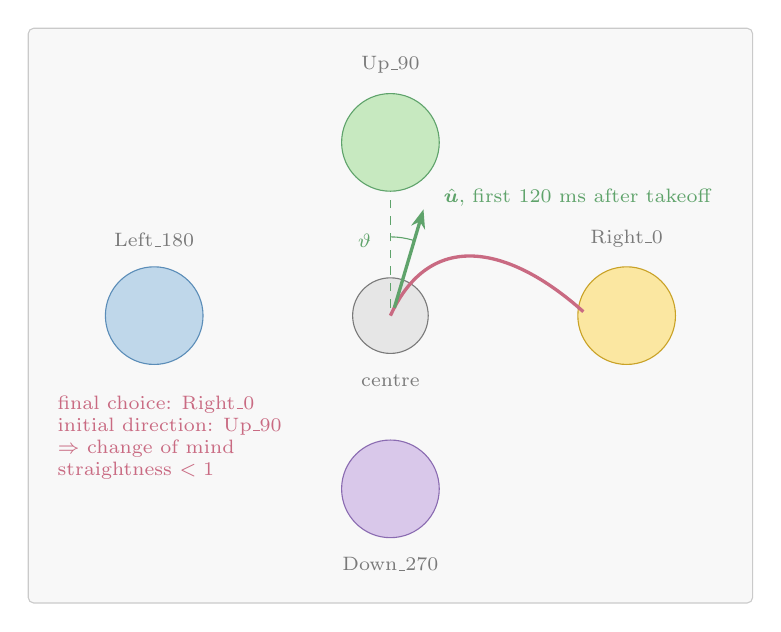
\begin{tikzpicture}[x=1cm,y=1cm]
\draw[fill=pgray!30, draw=dgray!40, rounded corners=2pt] (-4.6,-3.65) rectangle (4.6,3.65);
\draw[fill=pgreen, draw=dgreen] (0,2.2) circle (0.62);
\node[tag, anchor=south] at (0,2.95) {Up\_90};
\draw[fill=pblue, draw=dblue] (-3.0,0) circle (0.62);
\node[tag, anchor=south] at (-3.0,0.75) {Left\_180};
\draw[fill=pyellow, draw=dyellow] (3.0,0) circle (0.62);
\node[tag, anchor=south] at (3.0,0.75) {Right\_0};
\draw[fill=ppurple, draw=dpurple] (0,-2.2) circle (0.62);
\node[tag, anchor=north] at (0,-2.95) {Down\_270};
\draw[fill=pgray, draw=dgray] (0,0) circle (0.48);
\node[tag, anchor=north] at (0,-0.62) {centre};
% path
\draw[dpink, very thick] (0,0) .. controls (0.5,1.1) and (1.5,0.9) .. (2.45,0.05);
% heading arrow
\draw[-{Stealth[length=2.4mm]}, dgreen, very thick] (0.05,0.1) -- (0.42,1.35);
\node[tag, text=dgreen, anchor=west] at (0.55,1.5) {$\hat{\bm{u}}$, first 120 ms after takeoff};
\draw[dashed, dgreen] (0,0.1) -- (0,1.55);
\draw[dgreen] (0,1.0) arc (90:73:1.0);
\node[tag, text=dgreen, anchor=east] at (-0.12,0.95) {$\vartheta$};
\node[tag, text=dpink, anchor=west, align=left] at (-4.35,-1.55)
  {final choice: Right\_0\\initial direction: Up\_90\\$\Rightarrow$ change of mind\\straightness $< 1$};
\end{tikzpicture}
\caption{Change of mind from the initial heading. The unit vector over the first
120~ms after takeoff points at Up; the reach ends at Right. Screen $y$ grows
downward, which is why Up is encoded as $(0,-1)$ in Eq.~\eqref{eq:dirs}.}
\label{fig:com}
\end{figure}

The implementation is \code{initial\_heading}, which returns
$(\text{None}, \text{dist})$ when the cursor has not travelled far enough for
the direction to mean anything:

\begin{lstlisting}[language=Python]
t0   = result.move_takeoff_ms if np.isfinite(result.move_takeoff_ms) else gt[0]
mask = (gt >= t0) & (gt <= t0 + window_ms)
if mask.sum() < 2:
    return None, np.nan
seg  = gxy[mask]
v    = seg[-1] - seg[0]
dist = float(np.hypot(v[0], v[1]))
if dist < min_px:
    return None, dist
return (v / dist), dist
\end{lstlisting}

\noindent
Algorithm~\ref{alg:com} is the cell as a whole. Line~2 runs the five-stage
pipeline for the trial; lines 3--6 are Eq.~\eqref{eq:heading}, with the
early \code{continue} on line~6 marking a trial whose heading is unresolved
rather than guessing one; lines 7--8 are Eqs.~\eqref{eq:dirs}--\eqref{eq:angle}
and the comparison against the logged choice; line~10 is where the result meets
the difficulty axis of \S\ref{sec:timingcols}.

\begin{algorithm}[htbp]
\SetAlgoLined
\DontPrintSemicolon
\ForEach{trial with epochs \{decision, movement\}}{
  $r \leftarrow$ \code{TrajectoryProcessor.process}(trial)\;
  $t_0 \leftarrow r.\code{move\_takeoff\_ms}$ (or the first grid sample)\;
  $\text{seg} \leftarrow r.\code{grid\_xy}\big[\,t_0 \le t \le t_0 + 120\ \text{ms}\,\big]$\;
  $\bm{d} \leftarrow \text{seg}[\text{end}] - \text{seg}[0]$\;
  \If{$\|\bm{d}\| < 12$ px}{mark unresolved; \textbf{continue}\;}
  $\hat{\bm{u}} \leftarrow \bm{d}/\|\bm{d}\|$;\quad
  $D^\star \leftarrow \arg\max_D \hat{\bm{u}}\cdot\bm{e}_D$;\quad
  $\vartheta \leftarrow \arccos(\hat{\bm{u}}\cdot\bm{e}_{D^\star})$\;
  $\code{changed\_mind} \leftarrow [\,D^\star \ne \code{DirectionChosen}\,]$\;
}
Report the rate of changes of mind against distance to the fitted boundary
(Spearman $\rho$), and compare \code{straightness}, \code{TotalTime\_s} and
\code{DecisionTime\_s} between the two groups (Mann--Whitney)\;
\caption{\code{build\_change\_of\_mind} and \code{change\_of\_mind\_stats}.}
\label{alg:com}
\end{algorithm}

The 120~ms window is short on purpose: read on the 8~ms grid it spans 15 grid
points, and it ends well before the typical execution time. Two properties of
the acquisition chain matter here. The window is anchored on
\code{move\_takeoff\_ms}, which is derived from speed and therefore from the
time base; and the heading is a spatial quantity on the filtered grid, so it is
insensitive to a constant latency but not to a stretched or non-monotone time
axis, which would move the takeoff.

% ---------------------------------------------------------------------
\subsection{Where the timing columns enter the other analyses}
\label{sec:timingcols}
% ---------------------------------------------------------------------

\paragraph{Psychometric functions (1.5).} No kinematics and no timing. Each of
the $K-1$ category boundaries gets its own cumulative Gaussian with a lapse
term, fitted by binomial maximum likelihood to the ordinal splits
$P(\text{chosen} \ge 2)$ and $P(\text{chosen} \ge 3)$; 95\,\% intervals are
percentile bootstraps over the per-level binomial counts. Only
\code{ErrorType} matters here, through the lapse term, and only type 3 (hold
break after a target was chosen) reaches the fit: it puts a floor and a ceiling
on the curve, and fitting without a lapse absorbs those trials into the slope
and biases both $\mu$ and $\sigma$. Type 1 (early exit) never arrives, because
\code{ordinal\_choice\_table} keeps only \code{ChosenTarget} $\ge 1$ and the
source frame is \code{ANALYSIS\_DF} when it exists and
\code{drop\_early\_exits(FEATURES\_DF)} otherwise, so the cell no longer depends
on an earlier cell having filtered for it. A reduced stimulus set (three lengths)
cannot identify three free parameters per boundary, and the cell reports raw
proportions instead of a fit the data cannot support.

\paragraph{Chronometric functions (1.6).} Difficulty is the distance from each
trial's bar length to the nearest \emph{fitted} boundary
(\code{boundary\_distance}, using the $\mu$ values from 1.5 rather than the
nominal $[5.05, 6.40]$ deg VA), so it reflects where this subject placed the
criterion. \code{TotalTime\_s}, \code{DecisionTime\_s},
\code{ExecutionTime\_s} and \code{TakeoffToTargetTime\_s} are tested separately,
by Spearman $\rho$ and by linear regression, because the decision half is where
a difficulty effect belongs and a signature in the execution half would indicate
a motor confound. The fourth measure is the only one read off the trajectory
rather than off the task CSV, and it is the execution half timed from the
movement instead of from the geometry: \code{ExecutionTime\_s} starts when the
cursor leaves the centre circle, \code{TakeoffToTargetTime\_s} starts at the
takeoff, which is earlier by \code{takeoff\_lead\_ms}. The two therefore differ
by that lead, up to the residual between the task's own event marks and the
trajectory rows they were taken from. This is the
analysis most directly damaged by a clock defect: a session-long trend in
\code{DecisionTime\_s} would masquerade as anything correlated with trial order.

\paragraph{Sequential effects (1.7).} Post-error slowing uses the same timing
columns; direction perseveration uses \code{DirectionChosen} only. Because
\file{CenterOutTask.m} carries \code{prevTrialCorrect} across block boundaries,
the previous outcome is recomputed within each block and the first trial of
every block is dropped; the agreement rate against the logged column is printed
as a check on the CSV.

\paragraph{Error taxonomy and foil events (1.8).} \code{ErrorType} separates
type 2 (a target was chosen and it was the wrong one, the only category error)
from types 1 and 3 (motor or attention failures where no category was committed
to). Perceptual errors should concentrate near the boundary while motor errors
should be flat against difficulty, and pooling them is what makes a lapse look
like a discrimination failure. \code{foil\_events\_*.csv} is read here for the
per-entry record of every distractor touch during forgiving pre-training, which
gives a graded measure of uncertainty that a one-row-per-trial file cannot
express.

\paragraph{PCA, K-means, decoding (1.3, 1.4, 1.10).} These consume the feature
vector above; \code{takeoff\_to\_target\_ms} is in both the \code{PCA\_FEATURES}
list and the \code{DECODE\_PREFERRED} list, next to \code{move\_takeoff\_ms}.
\code{BarSizeVA\_deg} is held out when the target is \code{StimulusGroup}, since
the category is a deterministic function of the bar length and leaving it in
would score a lookup table. A permutation test sets the chance level for the
actual sample size and class balance rather than assuming
$1/n_{\text{classes}}$, and the adjusted Rand index of the K-means solution is
printed alongside for comparison. K-means chooses $k$ by silhouette; when that
choice is not 2 and \code{SHOW\_K2\_OVERLAY} is \code{True} (the default), the
cell additionally fits $k = 2$ and cross-tabulates it against \code{IsCorrect}.
The fixed-$k$ view exists because the silhouette answers ``how many compact
clusters are in this feature space'' and not ``do the two outcome labels
separate'', and only the second question is the one the panel is read for.

\paragraph{Figure colours.} \code{CATEGORY\_COLORS} is derived from the rig's
own category colours rather than from a plotting palette. \code{ColorCategoryMap.m}
paints category 1 orange, 2 green and 3 blue, and \code{ConfigOrgParams.m}
exposes the same three as \code{color3CatShort/Mid/Long}; the single-session
notebook reads them from this session's \code{params\_<runTag>.mat}
(\code{SESSION\_PARAMS.color3cat\_hex}) when the snapshot is present and falls
back to the literals \code{FFA500}, \code{00FF00}, \code{0000FF} otherwise. Each
is then passed through \code{\_pastelize}, which converts to HLS, keeps the hue
and pins lightness and saturation to $(0.72, 0.60)$. Keeping the hue is what
makes a figure agree with what the screen painted; pinning the other two is what
keeps three colours chosen for a dark booth display from being read as ink.

% =====================================================================
\section{Parameter reference: what to modify, where, and what it does}
\label{sec:params}
% =====================================================================

% ---------------------------------------------------------------------
\subsection{Online chain (MATLAB)}
\label{sec:params-online}
% ---------------------------------------------------------------------

\begin{longtable}{@{}P{4.0cm}P{1.65cm}P{3.55cm}P{5.75cm}@{}}
\toprule
Parameter & Default & Location & Effect and guidance \\
\midrule
\endfirsthead
\toprule
Parameter & Default & Location & Effect and guidance \\
\midrule
\endhead
\code{rz2SampleRateHz} ($f_s^{\text{seed}}$) & 939.0024 &
  \file{ConfigOrgParams.m}, read in \file{SetupRZ2Joystick.m} &
  Seed of the clock map slope and centre of its clamp (Eq.~\eqref{eq:slope}).
  Should equal $24414.0625/\code{downsample}$; confirm with
  \code{getSamplingRates}. A wrong seed costs a warm-up, not a session, but a
  seed outside $\pm 1\%$ of reality makes the clamp bind and trips the
  monitor. \\
\code{rz2ClockWindow} ($L$) & 600 & \file{ConfigOrgParams.m} &
  Observations (one per accepted drain) in the sliding OLS window
  ($\approx 16$ obs/s on this link, so $\approx 40$ s). Slope window only. \\
\code{rz2ClockMinSpanSec} & 30 s & \file{ConfigOrgParams.m} &
  Index span the slope window must cover before OLS replaces the seed
  (Eq.~\eqref{eq:slope}). Below it the seed is the better estimate. \\
\code{rz2ClockMaxRateDev} ($\delta$) & 0.01 & \file{ConfigOrgParams.m} &
  Fractional clamp on the slope around the seed. The seed is rig-confirmed to
  $\sim 0.04\%$, so a fit that wants to leave it by more than 1\,\% is noise or
  a corrupt index stream. \\
\code{rz2ClockOffset\-Window} & 100 & \file{ConfigOrgParams.m} &
  Most recent observations the intercept quantile is taken over
  (Eq.~\eqref{eq:offset}). Must slide: a window that never fills ratchets. \\
\code{rz2ClockOffset\-Quantile} & 0.10 & \file{ConfigOrgParams.m} &
  Residual quantile the intercept is anchored on; 0 would be the strict
  minimum, which one early packet can drag. \\
\code{rz2ClockMaxSlewSec} & 2 ms & \file{ConfigOrgParams.m} &
  Largest move one refit may apply to $\hat t$ at the newest index
  ($\times 5$ during the first 100 fits). Keeps the output monotone by design. \\
\code{rz2SkewWarnSec},\newline\code{rz2SkewAbortSec} & 0.05, 0.20 s &
  \file{ConfigOrgParams.m} $\rightarrow$ \file{ClockSkewMonitor.m} &
  Warn threshold on the instantaneous $|\varsigma_k|$; abort threshold on the
  90-frame median. Warn is one epoch's jitter; abort is the point where every
  sample-anchored window is measurably shorter than configured. \\
\code{rz2SkewWindowFrames} & 90 & \file{ConfigOrgParams.m} $\rightarrow$
  \file{ClockSkewMonitor.m} &
  Frames in the sustained (median) window the abort is judged on
  ($\approx 1.5$ s at 60 fps). \\
\code{nonFiniteAbortRun} & $10 \times$ window &
  \file{ClockSkewMonitor.m} (constructor default) &
  Consecutive non-finite skew readings that trip the abort ($\approx 900$
  frames, 15 s). Catches a clock map that never anchors because the queue never
  clears. \\
\code{rz2MaxSamples\-PerDrain} ($M$) & 2048 & \file{ConfigOrgParams.m} &
  Per-frame drain ceiling. Governs backlog recovery time $k^\star$
  (Eq.~\eqref{eq:backlog}); too large risks a long parse inside one frame, too
  small makes recovery slow. Lower it only if frames stutter while draining. \\
\code{rz2CapWarnFrames} & 60 & \file{ConfigOrgParams.m} &
  Consecutive capped frames before the \code{rz2:drainCapped} warning
  ($\approx 1$ s). \\
\code{rz2InputBufferSize} & 4\,194\,304 B & \file{ConfigOrgParams.m} &
  Socket receive buffer (and the OS receive buffer on the NIO channel). Must
  exceed the largest burst ($\approx 29$ B/sample). \\
\code{rz2InputDatagram\-PacketSize} & 8192 B & \file{ConfigOrgParams.m} &
  Largest datagram the legacy \code{udp()} object returns whole; its 512-byte
  default truncated every relay datagram. Load-bearing only on the legacy
  transport. \\
\code{rz2UdpPort},\newline\code{rz2RelaySourcePort} & 8831, 8832 &
  \file{ConfigOrgParams.m} &
  Must match the relay; the legacy object filters datagrams by remote
  host and port. \\
\code{rz2ScaleX},\newline\code{rz2ScaleY} ($s_x, s_y$) & 1, 1 &
  \file{ConfigOrgParams.m}, console ``RZ2 gain'' &
  Pixels per unit deflection as a fraction of $W, H$ (Eq.~\eqref{eq:map}); sign
  inverts the axis. Changing them changes the CSV pixel coordinates, so the
  offline geometry must match the session. \\
\code{rz2OffsetY} ($o_y$) & 0 & \file{ConfigOrgParams.m} &
  Vertical rest-position correction in px. \\
\code{joyGain} & $-1.3$ & console, \file{ReadCursorPosition.m} &
  USB-joystick counterpart of $s_x = s_y$. \\
\code{moveOversample},\newline\code{moveOversampleDt} & 1, 0.008 s &
  \file{CenterOutTask.m} (USB and mouse only) &
  Extra reads per frame and their spacing; 8 ms matches the joystick's measured
  HID update interval. Skipped entirely on \code{rz2adc}. \\
\code{movementExportEpochs} & $\{6,7,8\}$ & \file{CenterOutTask.m} &
  Rows kept in \code{trajectory\_movement\_*.csv}. Removing 8 drops the hold
  flags offline. \\
\code{trajChunk} & 200\,000 & \file{CenterOutTask.m} &
  Growth increment of \code{trajBuf}; performance only. \\
\midrule
Synapse \code{downsample} ($D$) & 26 & Synapse runtime parameter (Computer 1) &
  Sets $f_s = 24414.0625/D$ (Eq.~\eqref{eq:fs}). Can reset to 1 on a Synapse
  restart; confirm at session start. \\
\code{JOY\_RANGE} & 4.6 V & \file{InitJoystickRelay.m} &
  Volts mapped to $\pm 1$; values beyond are clipped. Changing it rescales
  every $v$ and therefore every pixel coordinate. \\
\code{RELAY\_HZ} & 169.4 & \file{InitJoystickRelay.m} &
  Relay cycle rate; sets datagrams/s and the per-cycle batch
  ($\approx f_s/169.4$). In write-index mode it does not set the read rate. \\
\code{MAX\_READ\_PER\_CYCLE},\newline\code{MAX\_SAMPLES\_PER\_DGRAM} & 4096, 17 &
  \file{InitJoystickRelay.m} &
  Burst ceiling per cycle, and lines per datagram ($17 \times 30$ B worst case
  $= 510 < 512$). \\
\code{IDX\_Y\_CHECK\_EVERY},\newline\code{IDX\_Y\_TOL} & 10, 2 &
  \file{InitJoystickRelay.m} &
  Cadence of the Y write-index consistency read and the divergence that reverts
  to reading both every cycle. \\
\code{BUF\_SIZE} ($B$) & 100\,000 & \file{InitJoystickRelay.m} (must match the
  \code{SerStore} size) &
  Ring size; $B/f_s \approx 106$ s is how long Computer 1 may stall before
  samples are overwritten. \\
\code{WRITE\_IDX\_TAG\_X/Y} & \code{'???'} & \file{InitJoystickRelay.m} &
  Non-empty enables write-index mode, but only after both names are found in
  \code{getParameterNames} on their gizmo at startup; a missing one warns and
  resets both to \code{''} (\S\ref{sec:c1}). \code{N\_READ},
  \code{WRITE\_FS} $=1017$, \code{READ\_FS}, \code{RECAL\_*} serve only the
  legacy fallback, which is reachable but tuned to a write rate that was never
  real. \\
\bottomrule
\end{longtable}

% ---------------------------------------------------------------------
\subsection{Offline chain (notebook, section 1.1 cell)}
\label{sec:params-offline}
% ---------------------------------------------------------------------

\begin{longtable}{@{}P{4.0cm}P{1.65cm}P{3.55cm}P{5.75cm}@{}}
\toprule
Parameter & Default & Location & Effect and guidance \\
\midrule
\endfirsthead
\toprule
Parameter & Default & Location & Effect and guidance \\
\midrule
\endhead
\code{hampel\_half\_window} ($h$) & 3 & \code{PipelineProfile} $\rightarrow$
  \code{HampelScreen} &
  Window $2h+1$. At 939 Hz, 7 samples is $\approx 7.5$ ms (58 ms on the USB
  path); a wider window tolerates longer dropouts but starts to treat fast real
  onsets as outliers. \\
\code{hampel\_n\_sigma} ($n_\sigma$) & 3.0 & same &
  Threshold in robust-$\sigma$ units. Lower is more aggressive. \\
\code{meas\_sigma\_px}\newline($\sigma_{\text{meas}}$) & 2.0 & \code{PipelineProfile}\newline
  $\rightarrow$ \code{Kalman\-Trajectory\-Smoother} &
  Measurement noise s.d. in px. Only the ratio $q/R$ matters for the estimate. \\
\code{jerk\_sigma\_px\_s3}\newline($\sigma_{\text{jerk}}$) & $10^5$ & same &
  Process-noise s.d.\ of jerk; $q = \sigma_{\text{jerk}}^2$ in Eq.~\eqref{eq:Q}.
  Rough smoothing corner $(q/R)^{1/6}$: $10^5 \rightarrow 5.9$ Hz,
  $10^4 \rightarrow 2.7$ Hz, $10^6 \rightarrow 12.6$ Hz. Increasing it makes the
  stage a near pass-through. \\
\code{gate\_sigma} ($\gamma$) & $\infty$ & same &
  $\chi^2$ innovation gate. A finite value rejects measurements the model finds
  implausible; use with care, since a rejected update costs delays. \\
\code{drop\_unindexed\_rows} & \code{True} on \code{rz2adc} &
  \code{PIPELINE\_PROFILES} &
  Removes \code{RZ2Idx} $=$ \code{NaN} rows when the file is read
  (\S\ref{sec:reading}). Off on \code{usb}, where every row is NaN. \\
\code{RZ2\_MAX\_MEDIAN\_\-STEP\_MS} & 3.0 ms & module constant &
  Threshold of the fallback source rule, Eq.~\eqref{eq:detect}. RZ2 delivers
  $\approx 1.06$ ms steps, USB $\approx 8$ ms. \\
\code{INPUT\_SOURCE\_\-OVERRIDES} & \{\} & module constant &
  Maps a run tag (or part of one) to a source, bypassing Eq.~\eqref{eq:detect}. \\
\code{grid\_dt\_s} ($\Delta$),\newline\code{GRID\_DT\_S} & 0.008 &
  module constant, passed into \code{TrajectoryProcessor} &
  Resampling step (125 Hz). Also sets $f_s$ for the Butterworth and $\Delta$ in
  the Savitzky--Golay derivative. Must satisfy $f_c < 1/(2\Delta)$. \\
\code{CUTOFF\_HZ} ($f_c$) & 6.0 & module constant &
  Butterworth design cutoff; effective two-pass $-3$ dB at $0.802 f_c$
  (Eq.~\eqref{eq:effcut}). Note the class default is 20 Hz; the processor always
  overrides it with this constant. \\
\code{EFFECTIVE\_CUTOFF\_HZ} & 4.82 Hz & computed &
  $f_c$ mapped through the prewarped axis; used in figure titles so they stay
  correct when $f_c$ or $\Delta$ change. \\
\code{Butterworth\-Lowpass.N\_FACT} ($n_f$) & 6 & class attribute &
  Reflection pad length; matches \code{filtfilt}'s default for a second-order
  section. \\
\code{SAVGOL\_WINDOW} ($w$) & 11 & module constant &
  Derivative window in grid samples ($w\Delta = 88$ ms). Larger smooths
  acceleration more and lowers peaks. Must be odd. \\
\code{SAVGOL\_POLYORDER} ($p$) & 3 & module constant &
  Local polynomial degree; must be $< w$. \\
\code{ACCEL\_PEAK\_\-PERCENTILE} & 99.0 & module constant &
  Percentile reported as peak acceleration. \\
\code{TAKEOFF\_SPEED\_\-FRAC\_CHOICE} & \code{"5\%"} & module constant,
  \code{globals().get} &
  Selects $\rho$ from \code{TAKEOFF\_SPEED\_FRAC\_OPTIONS} (\code{"5\%"} $=0.05$,
  \code{"10\%"} $=0.10$) into \code{MOVE\_SPEED\_FRAC}. Sets the takeoff
  threshold, Eq.~\eqref{eq:takeoff}, and therefore the start of the summary
  window. \\
\code{TAKEOFF\_PEAK\_CHOICE} & \code{"first"} & module constant,
  \code{globals().get} &
  \code{"first"} walks back from the first prominent local speed peak; any
  other value walks back from the global maximum over $\mathcal{S}$. Only
  differs on trials with more than one submovement. \\
\code{MULTI\_PEAK\_\-PROMINENCE\_FRAC} & 0.15 & module constant,
  \code{globals().get} &
  Prominence a local maximum needs, as a fraction of the largest speed in
  $\mathcal{S}$, to count as a peak in \code{find\_peaks} and therefore in
  \code{n\_speed\_peaks}. Lower it and ripple counts as a submovement. \\
\code{min\_move\_samples},\newline\code{min\_move\_dur\_s} & 5, \code{None} &
  \code{TrajectoryProcessor} &
  Under-resolved criteria, Eq.~\eqref{eq:flag1}. \\
\code{PIXEL\_PITCH\_MM}\newline$\rightarrow$ \code{CM\_PER\_PX} ($c$) & 0.3108 mm &
  module constants &
  Unit conversion for all cm quantities. \\
\code{MOVE\_EPOCHS} & $(6,7,8)$ or $(6,7)$ & module constant, per cell &
  Epoch codes loaded. The 1.1 cell uses $(6,7,8)$ so the hold flags have rows;
  the trajectory-EDA cell and the feature table use $(6,7)$. The summary window
  is bounded by target entry, so the choice does not change the summaries. \\
\code{INITIAL\_HEADING\_MS},\newline\code{MIN\_HEADING\_PX} & 120 ms, 12 px &
  change-of-mind cell &
  Window and minimum displacement for Eq.~\eqref{eq:heading}. \\
\code{NOMINAL\_BOUNDARIES} & $[5.05, 6.40]$ & chronometric cell &
  Fallback boundaries in deg VA; the fitted $\mu$ from 1.5 is used when
  available. \\
\code{CENTER\_DIAMETER\_PX},\newline\code{TARGET\_DIAMETER\_PX},\newline\code{CENTER\_TO\_TARGET\_\-DIST\_PX},\newline\code{TARGET\_DIST\_SCALE} &
  200, 180, 320, 1.27 & module constants, overridden by
  \code{params\_<runTag>.mat} &
  Geometry for the hold-instability threshold and the figure overlays. Now read
  from the session's own parameter snapshot when one exists
  (\S\ref{sec:reading}); the constants are the last fallback. \\
\code{EARLY\_EXIT\_CODE} & 1 & module constant, \code{globals().get} &
  \code{ErrorType} value that marks a trial ended without a target being
  chosen. Used twice: \code{run()} skips those trials and excludes them from the
  axis limits, and \code{drop\_early\_exits} removes them from the feature
  table. \\
\code{MAX\_TRAJ\_TIME\_MS} & 4000 ms & module constant &
  Hard upper limit of the shared trajectory time axis. Trials longer than this
  are drawn clipped and listed by Block/Trial/Attempt. \\
\code{SHOW\_K2\_OVERLAY} & \code{True} & clustering cell &
  When the silhouette picks $k \ne 2$, also fit $k = 2$ and cross-tabulate it
  against \code{IsCorrect}. \\
\code{EXCLUDE\_INVALID\_\-SESSIONS},\newline\code{INVALID\_SESSIONS} & \code{True}, 2
  entries & session loader &
  Sessions skipped with a printed reason (\S\ref{sec:offlineclock}). \\
\bottomrule
\end{longtable}

% ---------------------------------------------------------------------
\subsection{Recommended order of adjustment}
% ---------------------------------------------------------------------

\begin{enumerate}[leftmargin=*,itemsep=3pt]
\item Confirm $f_s$ at session start (Synapse \code{downsample}) and read the
teardown line \code{RZ2 clock: estimated write rate} together with the
accepted/refused counts. A persistent gap between seed and estimate means
\code{rz2SampleRateHz} should be updated to the measured value; ``all refused''
means a real backlog, not a clock problem.
\item Cross-check that estimate against the \code{OfflineClockFit} report for
the same session, which lives in the single-session notebook
(\S\ref{sec:offlineclock}). Two estimators, one data set: agreement is evidence,
disagreement localises the fault.
\item Keep $\sigma_{\text{jerk}}$ and $f_c$ on the same scale (they currently
are, $\approx 6$ Hz). If one is changed, revisit the other, and verify that
content above $1/(2\Delta)$ is negligible before resampling.
\item Change $w$ and $p$ only together with $\Delta$: the physical window is
$w\Delta$.
\item The screen geometry is read from \code{params\_<runTag>.mat}. Edit the
module constants only for sessions that predate that export, or supply a
\code{geometry\_spec*.json} beside the trial data.
\end{enumerate}

% =====================================================================
\section{Observations and open points in the current code}
\label{sec:observations}
% =====================================================================

These are properties of the version described above, found by reading it. They
are not defects unless stated; several are deliberate choices whose consequences
are worth having written down.

\begin{itemize}[leftmargin=*,itemsep=5pt]

\item \textbf{Consistent smoothing scales.} The Kalman defaults and the
Butterworth cutoff both imply a corner near 6 Hz (Eq.~\eqref{eq:corner} and
Eq.~\eqref{eq:effcut}), so the pipeline is not over-filtering relative to its own
stated bandwidth. The $(q/R)^{1/6}$ heuristic should be treated as an order of
magnitude, not a specification.

\item \textbf{The effective cutoff is 4.8 Hz, not 6 Hz.} Any report of the
filter should quote \code{EFFECTIVE\_CUTOFF\_HZ}, which the code computes from
$f_c$ and the grid rate, rather than the design parameter.

\item \textbf{The takeoff and the reported peak can belong to different
submovements.} \code{move\_takeoff\_ms} is walked back from the first
prominent peak (\code{TAKEOFF\_PEAK\_CHOICE} $=$ \code{"first"}), while
$v_{\text{peak}}$ is the maximum over the whole window. On a single-submovement
trial they coincide; on a corrected reach they do not, and that is deliberate.
Any analysis that pairs a peak speed with an onset should carry
\code{n\_speed\_peaks} alongside, and \code{peak\_vel\_time\_ms} says which
peak was reported.

\item \textbf{The summary window is now one mask.} Peak, mean and median of both
speed and acceleration are taken over $\mathcal{M}$ (5\,\% takeoff to target
entry, Eq.~\eqref{eq:summ}). This removes the earlier asymmetry in which the
peak was searched over the whole exported window while the means and medians
were restricted to the movement epoch, and it is what makes the summaries
independent of which epochs a given cell loads.

\item \textbf{Duplicate timestamps are dropped keeping the first sample.} On the
\code{rz2adc} path every duplicate is a cached row (write path 2), which carries
the previous row's time by design and no new position, so dropping it is
correct. The count is now reported per session in
\code{df.attrs["n\_duplicate\_ts"]} and per trial in
\code{TrialResult.n\_duplicate\_ts}. On the USB path a duplicate means the HID
driver returned a cached report, which is also information-free.

\item \textbf{The Hampel stage is inert during perfectly still holds}
($\mathrm{MAD}_i = 0$ guard, \S\ref{sec:hampel}). This fires more often on the
USB path, whose quantisation step is 5--20 px, than on the RZ2 path, whose wire
resolution is $\approx 0.2$ px.

\item \textbf{The clock map's floor latency is unmeasured.} It survives in $b$
as a constant, cancels in every within-trial difference, and shifts every
stimulus-to-response interval by that fixed amount. \code{DecisionTime\_s} is
therefore a reaction time plus an unknown constant, not plus a queue. Measuring
the constant needs a hardware loopback.

\item \textbf{The queue-clear gate trades coverage for correctness.} Only drains
that emptied the queue feed the estimator (Eq.~\eqref{eq:gate}). On a link that
is chronically a few datagrams behind but stable, most observations are refused
and the slope is estimated from the minority that cleared; the teardown
accepted/refused counts say how thin that minority was. If it is zero, the seed
stood in for the rate all session, and the report flags it. The non-finite abort
run of \S\ref{sec:skew} is the backstop for the case where it is zero for the
whole session.

\item \textbf{\code{WRITE\_FS} $= 1017$ on Computer 1 is an open item, not a
footnote.} It bends the ``ms behind head'' log line (7.7\,\% low) and
\file{VerifyWidxWidy.m}'s reference (\S\ref{sec:c1}). The planned fix is
measurement at relay startup rather than a new constant, so that the two
machines produce independent estimates of the same quantity.

\item \textbf{The write-index guard is a startup check, so a tag that dies
mid-session is still not caught.} \file{InitJoystickRelay.m} now proves both
tags exist with \code{getParameterNames} before write-index mode engages
(\S\ref{sec:c1}), which closes the silent-freeze path a repointed tag used to
open. It runs once, deliberately, to keep a fourth HTTP call out of the profiled
cycle. The residual case, a tag that stops resolving after the session has
started, remains undetectable through \code{getParameterValue}, which returns
rather than throws; the symptom would be \code{Samples=0/Dgrams=0} in the
5-second log with no warning. That is a reading habit, not a code change, unless
the failure ever appears.

\item \textbf{The legacy pacing path is now reachable but still mis-tuned.} A
missing tag drops the relay onto \code{READ\_FS} $= \code{N\_READ} \times
\code{RELAY\_HZ} = 1016.4$~Hz and the diff-peak recalibration, both set against
a write rate that was never real ($\approx 939$~Hz). The fallback is therefore a
loud degradation, which is what it should be, and not a second correct mode. It
inherits the \code{WRITE\_FS} open item of the previous bullet.

\item \textbf{\code{RZ2Idx} has two consumers offline, but only one of them in
every notebook.} It selects the pipeline profile and drops the cached rows
(\S\ref{sec:reading}) in both, and it supports the whole-session clock refit of
\S\ref{sec:offlineclock} in the single-session notebook only. The multi-session
notebook no longer runs that refit, so a session that is only ever seen in a
multi-session sweep has its time base classified but not checked. The analyses
still read \code{Time\_ms} as the time base; the refit is a check on it.
Re-deriving $\tau_i$ from the offline fit and re-running the pipeline on that
time base remains possible and is not currently done.

\item \textbf{The section 0.2 configuration cell is now inert.} It still sets
\code{MOVE\_SPEED\_FRAC} and \code{MOVE\_SPEED\_FRAC\_ALT} and prints both, but
the signal-processing cells overwrite \code{MOVE\_SPEED\_FRAC} from
\code{TAKEOFF\_SPEED\_FRAC\_OPTIONS[TAKEOFF\_SPEED\_FRAC\_CHOICE]} and no longer
read the alternate fraction at all, so editing either value there changes
nothing downstream while the printed line says it did. The threshold is now
changed through \code{TAKEOFF\_SPEED\_FRAC\_CHOICE}, and the cell's own markdown
(which still describes \code{move\_takeoff\_alt\_ms} as a second reference line
in the figures) describes a version that no longer exists. This is a
documentation defect in the notebook, not in the pipeline, and it is the kind
that silently costs an afternoon.

\item \textbf{The offline geometry now comes from the session.}
\code{ScreenGeometry.resolve} prefers \code{orgParams} in
\code{params\_<runTag>.mat}, so the notebook constants are a fallback rather
than something an analyst must remember to edit. Sessions recorded before that
snapshot existed still need the \code{geometry\_spec*} override or the
constants, and the printed line names which was used.

\item \textbf{Epoch loading differs between cells by design.} The 1.1 cell loads
$(6,7,8)$ and the feature table loads $(6,7)$. This no longer changes the
kinematic summaries (see the two bullets on the summary window above), but it does change
\code{hold\_dur\_ms}, \code{hold\_max\_speed\_cm} and \code{hold\_excursion\_px},
which are only computable where the target-hold rows are present.

\item \textbf{\code{drop\_early\_exits} is keyed on \code{ErrorType}, not on
timing.} It removes $\code{ErrorType} = 1$ and cross-checks against
\code{ChosenTarget}. A negative \code{DecisionTime\_s} is no longer a failure
mode the current code can produce (\S\ref{sec:oneclock}), so nothing filters on
it; if one ever appears in a new session it is a signal, not noise, and the
monotonicity warning and the offline clock fit are where to look.

\end{itemize}


\end{document}
